% Options for packages loaded elsewhere
\PassOptionsToPackage{unicode}{hyperref}
\PassOptionsToPackage{hyphens}{url}
%
\documentclass[
]{article}
\usepackage{amsmath,amssymb}
\usepackage{iftex}
\ifPDFTeX
  \usepackage[T1]{fontenc}
  \usepackage[utf8]{inputenc}
  \usepackage{textcomp} % provide euro and other symbols
\else % if luatex or xetex
  \usepackage{unicode-math} % this also loads fontspec
  \defaultfontfeatures{Scale=MatchLowercase}
  \defaultfontfeatures[\rmfamily]{Ligatures=TeX,Scale=1}
\fi
\usepackage{lmodern}
\ifPDFTeX\else
  % xetex/luatex font selection
\fi
% Use upquote if available, for straight quotes in verbatim environments
\IfFileExists{upquote.sty}{\usepackage{upquote}}{}
\IfFileExists{microtype.sty}{% use microtype if available
  \usepackage[]{microtype}
  \UseMicrotypeSet[protrusion]{basicmath} % disable protrusion for tt fonts
}{}
\makeatletter
\@ifundefined{KOMAClassName}{% if non-KOMA class
  \IfFileExists{parskip.sty}{%
    \usepackage{parskip}
  }{% else
    \setlength{\parindent}{0pt}
    \setlength{\parskip}{6pt plus 2pt minus 1pt}}
}{% if KOMA class
  \KOMAoptions{parskip=half}}
\makeatother
\usepackage{xcolor}
\usepackage[margin=1in]{geometry}
\usepackage{color}
\usepackage{fancyvrb}
\newcommand{\VerbBar}{|}
\newcommand{\VERB}{\Verb[commandchars=\\\{\}]}
\DefineVerbatimEnvironment{Highlighting}{Verbatim}{commandchars=\\\{\}}
% Add ',fontsize=\small' for more characters per line
\usepackage{framed}
\definecolor{shadecolor}{RGB}{248,248,248}
\newenvironment{Shaded}{\begin{snugshade}}{\end{snugshade}}
\newcommand{\AlertTok}[1]{\textcolor[rgb]{0.94,0.16,0.16}{#1}}
\newcommand{\AnnotationTok}[1]{\textcolor[rgb]{0.56,0.35,0.01}{\textbf{\textit{#1}}}}
\newcommand{\AttributeTok}[1]{\textcolor[rgb]{0.13,0.29,0.53}{#1}}
\newcommand{\BaseNTok}[1]{\textcolor[rgb]{0.00,0.00,0.81}{#1}}
\newcommand{\BuiltInTok}[1]{#1}
\newcommand{\CharTok}[1]{\textcolor[rgb]{0.31,0.60,0.02}{#1}}
\newcommand{\CommentTok}[1]{\textcolor[rgb]{0.56,0.35,0.01}{\textit{#1}}}
\newcommand{\CommentVarTok}[1]{\textcolor[rgb]{0.56,0.35,0.01}{\textbf{\textit{#1}}}}
\newcommand{\ConstantTok}[1]{\textcolor[rgb]{0.56,0.35,0.01}{#1}}
\newcommand{\ControlFlowTok}[1]{\textcolor[rgb]{0.13,0.29,0.53}{\textbf{#1}}}
\newcommand{\DataTypeTok}[1]{\textcolor[rgb]{0.13,0.29,0.53}{#1}}
\newcommand{\DecValTok}[1]{\textcolor[rgb]{0.00,0.00,0.81}{#1}}
\newcommand{\DocumentationTok}[1]{\textcolor[rgb]{0.56,0.35,0.01}{\textbf{\textit{#1}}}}
\newcommand{\ErrorTok}[1]{\textcolor[rgb]{0.64,0.00,0.00}{\textbf{#1}}}
\newcommand{\ExtensionTok}[1]{#1}
\newcommand{\FloatTok}[1]{\textcolor[rgb]{0.00,0.00,0.81}{#1}}
\newcommand{\FunctionTok}[1]{\textcolor[rgb]{0.13,0.29,0.53}{\textbf{#1}}}
\newcommand{\ImportTok}[1]{#1}
\newcommand{\InformationTok}[1]{\textcolor[rgb]{0.56,0.35,0.01}{\textbf{\textit{#1}}}}
\newcommand{\KeywordTok}[1]{\textcolor[rgb]{0.13,0.29,0.53}{\textbf{#1}}}
\newcommand{\NormalTok}[1]{#1}
\newcommand{\OperatorTok}[1]{\textcolor[rgb]{0.81,0.36,0.00}{\textbf{#1}}}
\newcommand{\OtherTok}[1]{\textcolor[rgb]{0.56,0.35,0.01}{#1}}
\newcommand{\PreprocessorTok}[1]{\textcolor[rgb]{0.56,0.35,0.01}{\textit{#1}}}
\newcommand{\RegionMarkerTok}[1]{#1}
\newcommand{\SpecialCharTok}[1]{\textcolor[rgb]{0.81,0.36,0.00}{\textbf{#1}}}
\newcommand{\SpecialStringTok}[1]{\textcolor[rgb]{0.31,0.60,0.02}{#1}}
\newcommand{\StringTok}[1]{\textcolor[rgb]{0.31,0.60,0.02}{#1}}
\newcommand{\VariableTok}[1]{\textcolor[rgb]{0.00,0.00,0.00}{#1}}
\newcommand{\VerbatimStringTok}[1]{\textcolor[rgb]{0.31,0.60,0.02}{#1}}
\newcommand{\WarningTok}[1]{\textcolor[rgb]{0.56,0.35,0.01}{\textbf{\textit{#1}}}}
\usepackage{graphicx}
\makeatletter
\def\maxwidth{\ifdim\Gin@nat@width>\linewidth\linewidth\else\Gin@nat@width\fi}
\def\maxheight{\ifdim\Gin@nat@height>\textheight\textheight\else\Gin@nat@height\fi}
\makeatother
% Scale images if necessary, so that they will not overflow the page
% margins by default, and it is still possible to overwrite the defaults
% using explicit options in \includegraphics[width, height, ...]{}
\setkeys{Gin}{width=\maxwidth,height=\maxheight,keepaspectratio}
% Set default figure placement to htbp
\makeatletter
\def\fps@figure{htbp}
\makeatother
\setlength{\emergencystretch}{3em} % prevent overfull lines
\providecommand{\tightlist}{%
  \setlength{\itemsep}{0pt}\setlength{\parskip}{0pt}}
\setcounter{secnumdepth}{-\maxdimen} % remove section numbering
\usepackage{fancyhdr}
\usepackage{amsmath}
\pagestyle{fancy}
\fancyhead[CO,CE]{STAT3017/STAT6017 - Big Data Statistics - Sem 2 2023}
\fancyhead[LO,LE]{}
\fancypagestyle{plain}{\pagestyle{fancy}}
\renewcommand{\headrulewidth}{0.4pt}
\ifLuaTeX
  \usepackage{selnolig}  % disable illegal ligatures
\fi
\IfFileExists{bookmark.sty}{\usepackage{bookmark}}{\usepackage{hyperref}}
\IfFileExists{xurl.sty}{\usepackage{xurl}}{} % add URL line breaks if available
\urlstyle{same}
\hypersetup{
  pdftitle={Assignment 5},
  pdfauthor={Songze Yang u7192786},
  hidelinks,
  pdfcreator={LaTeX via pandoc}}

\title{Assignment 5}
\author{Songze Yang u7192786}
\date{}

\begin{document}
\maketitle

\subsection{Question 1}\label{question-1}

Consider two p-dimensional populations with covariance matrices \(I_p\)
and \((Ip + \Delta)\) where

\[
\Delta := diag(\delta_1, \delta_2, 0,.., 0)
\]

with \(\delta_1, \delta_2 \in. R\). Suppose we had p-dimensional random
samples \(x_1, . . . , x_{m+1} \sim Np(0, I_p)\) from the first
population and p-dimensional random samples
\(z_1, ..., z_n+1 \sim N(0, I_p + \Delta)\) from the second. We stack
these random samples to obtain the data matrices \(X\) and \(Z\) and
sample covariance matrices

\[
S_1 := \frac{1}{m}XX^T, \ 
S_2 := \frac{1}{n}ZZ^T, \ 
S := S_2^{-1}S_1.
\]

a. Assume \(n, m, p \rightarrow \infty\) such that
\(y_p := p/n \rightarrow y \in (0, 1)\) and
\(c_p := p/m \rightarrow c > 0\). Take \(\delta_1 = \delta_2 = 0\),
\(y = 1/4\), and \(c = 3/4\), what is the lower bound \(a\) and the
upper bound \(b\) of the limiting spectral distribution of \(S\)? For
each, give a formula in terms of \(c\) and \(y\). Also give a numerical
value.

\paragraph{\texorpdfstring{\textbf{Answer to question 1
(a)}:}{Answer to question 1 (a):}}\label{answer-to-question-1-a}

When the \(\delta_1 = \delta_2 = 0\), the \(I_p + \Delta = I_p\). We can
see that the \(X\) and \(Z\) satisfy the null case where
\(\Sigma_1 = \Sigma_2 = I_p\). Thus, this falls in the case that the
matrix entry \(x_{ij}\) are \(i.i.d.\) random variables with mean zero
and variance \(1\), \(y_p := p/n \rightarrow y \in (0, 1)\) and
\(c_p := p/m \rightarrow c > 0\). The Fisher LSD \(f_{c, y}\) is

\[
f_{c,y}(x) = \begin{cases} \frac{(1-y) \sqrt{(b-x)(x-a)}}{2\pi x (c+xy)} & \text{when } a \leq x \leq b, \\0 & \text{otherwise},\end{cases}
\]

where the upper bound \(a\) and lower bound \(b\) is:

\[
a = \left( \frac{1 - h}{1 - y} \right)^2 \\
b = \left( \frac{1 + h}{1 - y} \right)^2 \\
h = \sqrt{c + y - cy}
\]

Plugging in \(c = \frac{3}{4}\) and \(y = \frac{1}{4}\), we have:

\begin{Shaded}
\begin{Highlighting}[]
\NormalTok{c }\OtherTok{=} \DecValTok{3}\SpecialCharTok{/}\DecValTok{4}
\NormalTok{y }\OtherTok{=} \DecValTok{1}\SpecialCharTok{/}\DecValTok{4}
\NormalTok{h }\OtherTok{=} \FunctionTok{sqrt}\NormalTok{(c }\SpecialCharTok{+}\NormalTok{ y }\SpecialCharTok{{-}}\NormalTok{ c}\SpecialCharTok{*}\NormalTok{y)}
\NormalTok{a }\OtherTok{=}\NormalTok{ (}\DecValTok{1} \SpecialCharTok{{-}}\NormalTok{ h)}\SpecialCharTok{\^{}}\DecValTok{2}\SpecialCharTok{/}\NormalTok{(}\DecValTok{1} \SpecialCharTok{{-}}\NormalTok{ y)}\SpecialCharTok{\^{}}\DecValTok{2}
\NormalTok{b }\OtherTok{=}\NormalTok{ (}\DecValTok{1} \SpecialCharTok{+}\NormalTok{ h)}\SpecialCharTok{\^{}}\DecValTok{2}\SpecialCharTok{/}\NormalTok{(}\DecValTok{1} \SpecialCharTok{{-}}\NormalTok{ y)}\SpecialCharTok{\^{}}\DecValTok{2}
\NormalTok{a}
\end{Highlighting}
\end{Shaded}

\begin{verbatim}
## [1] 0.01728776
\end{verbatim}

\begin{Shaded}
\begin{Highlighting}[]
\NormalTok{b}
\end{Highlighting}
\end{Shaded}

\begin{verbatim}
## [1] 6.427157
\end{verbatim}

We have \(a = 0.01729\) and \(b = 6.42716\).

b. Suppose that \(\delta_1 = −\epsilon\) and \(\delta_2 = +\epsilon\)
for \(\epsilon = 1/10\). Would you expect \(S\) to have eigenvalues
smaller than \(a\) and larger than \(b\) in that case?

\paragraph{\texorpdfstring{\textbf{Answer to question 1
(b)}:}{Answer to question 1 (b):}}\label{answer-to-question-1-b}

By theorem 3.1 of \textbf{{[}B{]}}, we have the phase transition of the
extreme eigenvalues of Fisher matrix \(F\) follows:

\[ 
\lambda_i = 
\begin{cases} 
\phi(a_i), & \text{if } |a_i - \gamma| > \gamma\sqrt{c + y - cy} \\
b, & \text{if } 1 < a_i \leq \gamma\{1 + \sqrt{c + y - cy}\} \\
b_1, & \text{if } \gamma\{1 - \sqrt{c + y - cy}\} \leq a_i < 1 
\end{cases}
\]

Where the \(\phi\) function is in the form of:

\[
\phi(x) = \frac{\gamma x (x - 1 + c)}{x - \gamma}, \quad x \neq \gamma 
\]

The \(\gamma = 1/(1 − y) \in (1, \infty)\). The paper assume the spike
eigenvalues \(a_i\) is for \(\Omega_M\) in \(\Sigma_p\):

\[
\Sigma_p = \begin{pmatrix}\Omega_M & 0 \\0 & I_{p-M}\end{pmatrix}
\]

which can be written in form of
\(\Omega_M = U \, \text{diag}(a_1, \ldots, a_1, \ldots, a_k, \ldots, a_k) U^*\),
where \(U\) is a \(M \times M\) orthogonal matrix.

There is a mismatch between our notation and the notation in the paper.
In the paper \textbf{{[}B{]}}, it is assume that \(\Sigma_1 = \Sigma_p\)
and \(\Sigma_2 = I_p\). However, we assume the opposite in our case.
Therefore, we will need to scale the value in our case properly. The
Fisher matrix \(F = S^{-1}_2 S_1\) are invariant under the
transformation \(S_1 \mapsto \Sigma^{-1/2}_2 S_1 \Sigma^{-1/2}_2\),
\(S_2 \mapsto \Sigma^{-1/2}_2 S_2 \Sigma^{-1/2}_2\).

Thus, let's scale the \(S_2\) by
\(\Sigma^{-1/2}_2 =(I_p +\Delta)^{-1/2} = diag(\frac{1}{\sqrt{1+\delta_1}}, \frac{1}{\sqrt{1+\delta_2}},1,...,1)\).
Thus, \(\Sigma^{-1/2}_2 S_1 \Sigma^{-1/2}_2\) will be equal to
\(diag(\frac{1}{(1+\delta_1)}, \frac{1}{(1+\delta_2)},1,...,1)\).

In our formulation, the \(\Omega_M\) is equal to
\(diag(\frac{1}{1 + \delta_1}, \frac{1}{1+ \delta_2})\), where the
eigenvalues of this matrix are
\(a_1 = \frac{1}{1 + \delta_1}, a_2 = \frac{1}{1+ \delta_2}\). Thus,
Let's check their phase transition.

\begin{Shaded}
\begin{Highlighting}[]
\NormalTok{gamma }\OtherTok{=} \DecValTok{1}\SpecialCharTok{/}\NormalTok{(}\DecValTok{1} \SpecialCharTok{{-}}\NormalTok{ y)}
\NormalTok{a1 }\OtherTok{=} \DecValTok{1}\SpecialCharTok{/}\NormalTok{(}\DecValTok{1} \SpecialCharTok{{-}} \DecValTok{1}\SpecialCharTok{/}\DecValTok{10}\NormalTok{)}
\NormalTok{a2 }\OtherTok{=} \DecValTok{1}\SpecialCharTok{/}\NormalTok{(}\DecValTok{1} \SpecialCharTok{+} \DecValTok{1}\SpecialCharTok{/}\DecValTok{10}\NormalTok{)}
\FunctionTok{abs}\NormalTok{(a1 }\SpecialCharTok{{-}}\NormalTok{ gamma) }\SpecialCharTok{\textgreater{}}\NormalTok{ gamma}\SpecialCharTok{*}\NormalTok{h}
\end{Highlighting}
\end{Shaded}

\begin{verbatim}
## [1] FALSE
\end{verbatim}

\begin{Shaded}
\begin{Highlighting}[]
\FunctionTok{abs}\NormalTok{(a2 }\SpecialCharTok{{-}}\NormalTok{ gamma) }\SpecialCharTok{\textgreater{}}\NormalTok{ gamma}\SpecialCharTok{*}\NormalTok{h}
\end{Highlighting}
\end{Shaded}

\begin{verbatim}
## [1] FALSE
\end{verbatim}

Therefore, we do not expect \(S\) to have eigenvalues smaller than \(a\)
and larger than \(b\).

\begin{enumerate}
\def\labelenumi{(\alph{enumi})}
\setcounter{enumi}{2}
\tightlist
\item
  In the paper {[}A{]} (see also {[}B{]}) it is suggested that the
  largest eigenvalue \(\lambda_1\) of \(\mathbf{S}\), scaled as
  \(\frac{\lambda_1 - b}{sp}\) where \(b\) is from question (a) and
  \(s_p := \left( \frac{1}{m} (\sqrt{m} + \sqrt{p})(\sqrt{\frac{1}{m}} + \frac{1}{\sqrt{p}}) \right)^{1/3}\),
  behaves like a Tracy-Widom distribution of order 1. Show this using a
  simulation in the case \(n = 400\), \(y_n = \frac{1}{4}\) and
  \(c_n = \frac{3}{4}\). Plot the histogram and compare it against the
  Tracy-Widom distribution of order 1.
\end{enumerate}

\paragraph{\texorpdfstring{\textbf{Answer to question 1
(c)}:}{Answer to question 1 (c):}}\label{answer-to-question-1-c}

\begin{Shaded}
\begin{Highlighting}[]
\NormalTok{n }\OtherTok{=} \DecValTok{400}
\NormalTok{sim.F.max.eigenvalues }\OtherTok{=} \ControlFlowTok{function}\NormalTok{(delta\_1, delta\_2, }\AttributeTok{n =} \DecValTok{400}\NormalTok{, c, y, }\AttributeTok{n\_sims =} \DecValTok{1}\NormalTok{) \{}
\NormalTok{  p }\OtherTok{=}\NormalTok{ n }\SpecialCharTok{*}\NormalTok{ y}
\NormalTok{  m }\OtherTok{=}\NormalTok{ p }\SpecialCharTok{/}\NormalTok{ c}
\NormalTok{  evalues }\OtherTok{=} \FunctionTok{c}\NormalTok{()}
  \ControlFlowTok{for}\NormalTok{ (sim }\ControlFlowTok{in} \DecValTok{1}\SpecialCharTok{:}\NormalTok{n\_sims) \{}
\NormalTok{    Sigma1 }\OtherTok{=} \FunctionTok{diag}\NormalTok{(p) }
\NormalTok{    Sigma2 }\OtherTok{=} \FunctionTok{diag}\NormalTok{(p) }\SpecialCharTok{+} \FunctionTok{diag}\NormalTok{(}\AttributeTok{x =} \FunctionTok{c}\NormalTok{(delta\_1, delta\_2, }\FunctionTok{rep}\NormalTok{(}\DecValTok{0}\NormalTok{, p }\SpecialCharTok{{-}} \DecValTok{2}\NormalTok{)), p)}
\NormalTok{    mu }\OtherTok{=} \FunctionTok{rep}\NormalTok{(}\DecValTok{0}\NormalTok{, p)}
\NormalTok{    X }\OtherTok{=} \FunctionTok{rmvn}\NormalTok{(m}\SpecialCharTok{+}\DecValTok{1}\NormalTok{, mu, Sigma1)}
\NormalTok{    Z }\OtherTok{=} \FunctionTok{rmvn}\NormalTok{(n}\SpecialCharTok{+}\DecValTok{1}\NormalTok{, mu, Sigma2)}
\NormalTok{    S1 }\OtherTok{=} \FunctionTok{cov}\NormalTok{(X)}
\NormalTok{    S2 }\OtherTok{=} \FunctionTok{cov}\NormalTok{(Z)}
\NormalTok{    FF }\OtherTok{=} \FunctionTok{solve}\NormalTok{(S2) }\SpecialCharTok{\%*\%}\NormalTok{ S1}
\NormalTok{    evalues }\OtherTok{=} \FunctionTok{c}\NormalTok{(evalues, }\FunctionTok{max}\NormalTok{(}\FunctionTok{eigen}\NormalTok{(FF, }\AttributeTok{only.values =} \ConstantTok{TRUE}\NormalTok{)}\SpecialCharTok{$}\NormalTok{values))}
\NormalTok{    \}}
\NormalTok{  evalues }
\NormalTok{\}}
\NormalTok{p }\OtherTok{=}\NormalTok{ n }\SpecialCharTok{*}\NormalTok{ y}
\NormalTok{m }\OtherTok{=}\NormalTok{ p }\SpecialCharTok{/}\NormalTok{ c}
\NormalTok{s\_p }\OtherTok{=}\NormalTok{ (}\DecValTok{1}\SpecialCharTok{/}\NormalTok{m }\SpecialCharTok{*}\NormalTok{ (}\FunctionTok{sqrt}\NormalTok{(m) }\SpecialCharTok{+} \FunctionTok{sqrt}\NormalTok{(p)) }\SpecialCharTok{*}\NormalTok{ (}\DecValTok{1}\SpecialCharTok{/}\FunctionTok{sqrt}\NormalTok{(m) }\SpecialCharTok{+} \DecValTok{1}\SpecialCharTok{/}\FunctionTok{sqrt}\NormalTok{(p)))}\SpecialCharTok{\^{}}\NormalTok{\{}\DecValTok{1}\SpecialCharTok{/}\DecValTok{3}\NormalTok{\}}
\NormalTok{lambdas }\OtherTok{=} \FunctionTok{sim.F.max.eigenvalues}\NormalTok{(}\AttributeTok{delta\_1 =} \SpecialCharTok{{-}}\DecValTok{1}\SpecialCharTok{/}\DecValTok{10}\NormalTok{, }\AttributeTok{delta\_2 =} \DecValTok{1}\SpecialCharTok{/}\DecValTok{10}\NormalTok{, }\AttributeTok{c =}\NormalTok{ c, }\AttributeTok{y =}\NormalTok{ y, }\AttributeTok{n\_sims =} \DecValTok{1000}\NormalTok{)}
\end{Highlighting}
\end{Shaded}

\begin{Shaded}
\begin{Highlighting}[]
\NormalTok{F1 }\OtherTok{=}\NormalTok{ (lambdas }\SpecialCharTok{{-}}\NormalTok{ b) }\SpecialCharTok{/}\NormalTok{ s\_p}
\NormalTok{hhh }\OtherTok{\textless{}{-}} \FunctionTok{hist}\NormalTok{(F1, }\AttributeTok{breaks=}\DecValTok{80}\NormalTok{, }\AttributeTok{xlim=}\FunctionTok{c}\NormalTok{(}\SpecialCharTok{{-}}\DecValTok{4}\NormalTok{,}\DecValTok{4}\NormalTok{))}
\end{Highlighting}
\end{Shaded}

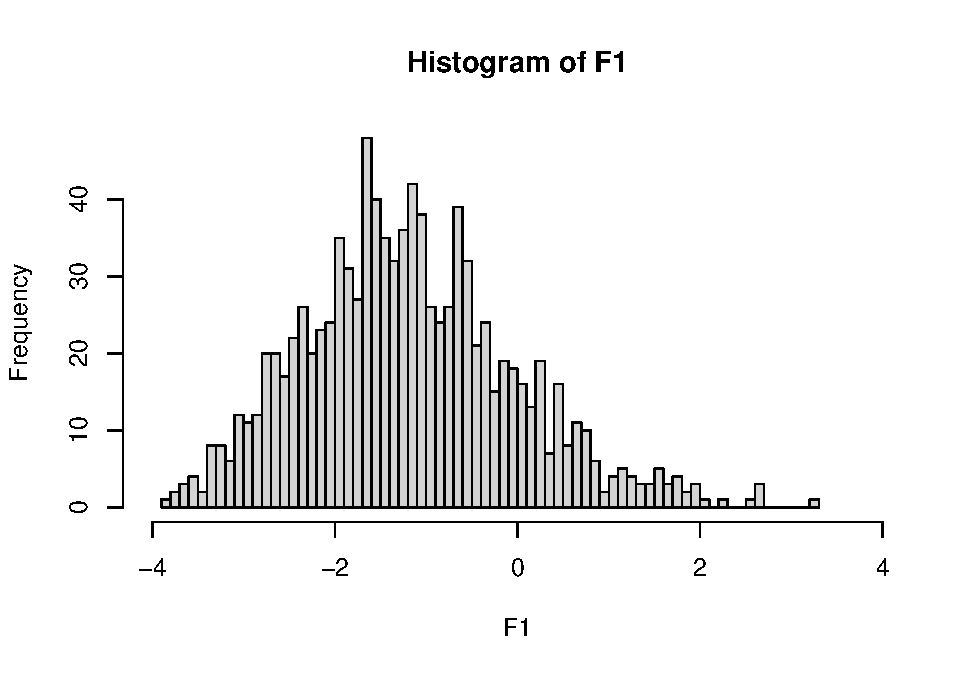
\includegraphics{A5_files/figure-latex/unnamed-chunk-4-1.pdf}

\begin{Shaded}
\begin{Highlighting}[]
\FunctionTok{plot}\NormalTok{(hhh}\SpecialCharTok{$}\NormalTok{mids, hhh}\SpecialCharTok{$}\NormalTok{density, }\AttributeTok{type=}\StringTok{"s"}\NormalTok{, }\AttributeTok{xlab=}\StringTok{""}\NormalTok{, }\AttributeTok{ylab=}\StringTok{""}\NormalTok{, }\AttributeTok{ylim=}\FunctionTok{c}\NormalTok{(}\DecValTok{0}\NormalTok{,}\DecValTok{1}\NormalTok{))}
\FunctionTok{curve}\NormalTok{(dtw, }\SpecialCharTok{{-}}\DecValTok{4}\NormalTok{, }\DecValTok{4}\NormalTok{, }\AttributeTok{lwd=}\DecValTok{2}\NormalTok{, }\AttributeTok{lty=}\DecValTok{3}\NormalTok{, }\AttributeTok{col=}\StringTok{"darkmagenta"}\NormalTok{, }\AttributeTok{add=}\ConstantTok{TRUE}\NormalTok{)}
\FunctionTok{title}\NormalTok{(}\AttributeTok{main=}\StringTok{"Distribution of largest eigenvalue vs. TW density"}\NormalTok{)}
\end{Highlighting}
\end{Shaded}

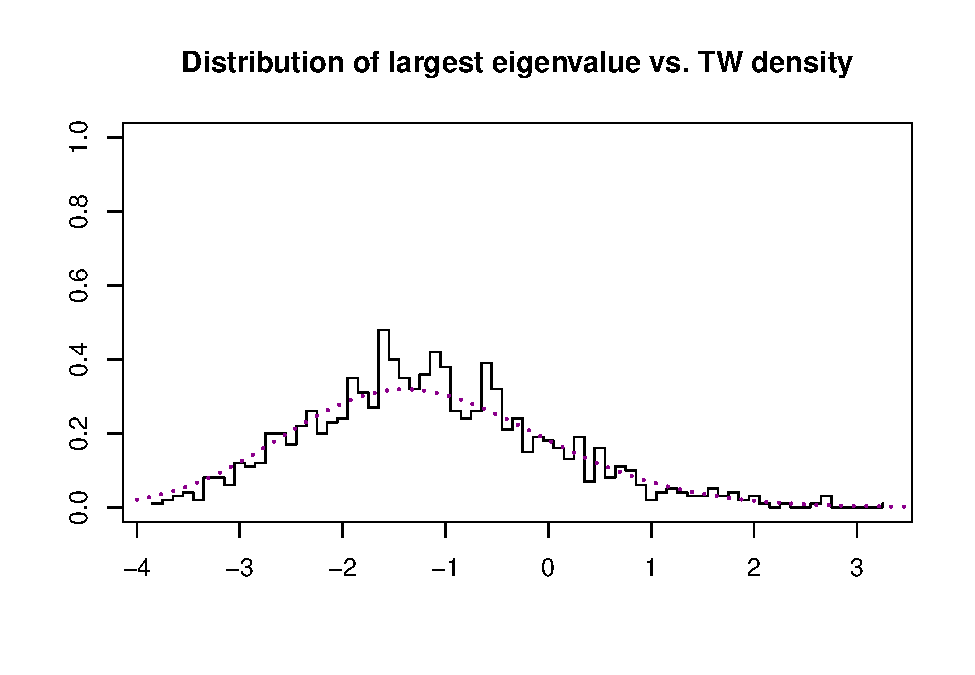
\includegraphics{A5_files/figure-latex/unnamed-chunk-4-2.pdf}

\begin{enumerate}
\def\labelenumi{(\alph{enumi})}
\setcounter{enumi}{3}
\tightlist
\item
  Considering {[}B{]}, suppose that \(\delta_1 < \ell\) and
  \(\delta_2 > \kappa\) for some choice of \(\ell\) and \(\kappa\). What
  would be the critical values of \(\ell\) and \(\kappa\) that would
  ensure you would have a large fundamental spike and a small
  fundamental spike? Give a formula for \(\ell\) and \(\kappa\) and also
  give a numerical value in the case \(y = \frac{1}{4}\) and
  \(c = \frac{3}{4}\).
\end{enumerate}

\paragraph{\texorpdfstring{\textbf{Answer to question 1
(d)}:}{Answer to question 1 (d):}}\label{answer-to-question-1-d}

From

\[
|a_i - \gamma| > \gamma\sqrt{c + y - cy}
\]

The critical values are \(a_i > \gamma * (1 + h)\) and
\(a_i < \gamma * (1 - h)\) for
\(a_1 = \frac{1}{1 + \delta_1}, a_2 = \frac{1}{1+ \delta_2}\). Let's
first explore the ranges: \(\sqrt{c + y -cy} >0\), \(\gamma>1\), thus
\(\gamma*(1+h) > 0\). Assume
\(0 \leq 1+\delta_1 \leq 1+\delta_2 \rightarrow \frac{1}{1+\delta_1}\geq\frac{1}{1+\delta_2}>0\)
and \(h <1 \rightarrow 1-h>0\), we have the following: \begin{align*}
\left\{
\begin{array}{ll}
\frac{1}{1+\delta_1} & > \gamma(1+h) \\
\frac{1}{1+\delta_2} & < \gamma(1-h) \\
\end{array}
\right.
&\Rightarrow
\left\{
\begin{array}{ll}
\delta_1 & < \frac{1}{\gamma(1+h)} - 1 \\
\delta_2 & > \frac{1}{\gamma(1-h)} -1 \\
\end{array}
\right.
\end{align*}

Assume
\(1 + \delta_1 \leq 0 \leq 1+\delta_2 \rightarrow \frac{1}{1+\delta_1}\leq\frac{1}{1+\delta_2}\)
and \(h <1 \rightarrow 1-h>0\), we have the following: \begin{align*}
\left\{
\begin{array}{ll}
\frac{1}{1+\delta_2} & > \gamma(1+h) \\
\frac{1}{1+\delta_1} & < \gamma(1-h) \\
\end{array}
\right.
&\Rightarrow
\left\{
\begin{array}{ll}
\delta_2 & < \frac{1}{\gamma(1+h)} - 1 \\
\delta_1 & > \frac{1}{\gamma(1-h)} -1 \\
\end{array}
\right.
\end{align*}

Otherwise, we do not have \(\ell\) and \(\kappa\) simultaneously. We can
see that upper critical value is always \(\frac{1}{\gamma(1-h)} - 1\)
and lower critical value is always \(\frac{1}{\gamma(1+h)} - 1\).

\begin{Shaded}
\begin{Highlighting}[]
\NormalTok{ell }\OtherTok{\textless{}{-}} \DecValTok{1}\SpecialCharTok{/}\NormalTok{(gamma}\SpecialCharTok{*}\NormalTok{(}\DecValTok{1} \SpecialCharTok{+}\NormalTok{ h)) }\SpecialCharTok{{-}} \DecValTok{1}
\NormalTok{kappa }\OtherTok{\textless{}{-}} \DecValTok{1}\SpecialCharTok{/}\NormalTok{(gamma}\SpecialCharTok{*}\NormalTok{(}\DecValTok{1} \SpecialCharTok{{-}}\NormalTok{ h)) }\SpecialCharTok{{-}} \DecValTok{1}
\NormalTok{ell}
\end{Highlighting}
\end{Shaded}

\begin{verbatim}
## [1] -0.6055513
\end{verbatim}

\begin{Shaded}
\begin{Highlighting}[]
\NormalTok{kappa}
\end{Highlighting}
\end{Shaded}

\begin{verbatim}
## [1] 6.605551
\end{verbatim}

If \(y = \frac{1}{4}\) and \(c = \frac{3}{4}\), we have
\(\ell = -0.60555\) and \(\kappa = 6.60555\).

\begin{enumerate}
\def\labelenumi{(\alph{enumi})}
\setcounter{enumi}{4}
\tightlist
\item
  Suppose that \(\delta_1 = \ell - \frac{1}{100}\) and
  \(\delta_2 = \kappa + \frac{1}{100}\) for your critical values of
  \(\kappa\) and \(\ell\) you found in (d), then give a formula for each
  of the two locations where you think the spike eigenvalues will
  cluster around and also a numerical value for each.
\end{enumerate}

Also, perform a simulation experiment to illustrate this phenomena. That
is, sample data and plot a histogram of eigenvalues of \(\mathbf{S}\),
compare it to the theoretical density expected if
\(\delta_1 = \delta_2 = 0\), and plot the location where you expect
spike eigenvalues to cluster around. Take \(n = 400\),
\(y_n = \frac{1}{4}\), and \(c_n = \frac{3}{4}\).

\paragraph{\texorpdfstring{\textbf{Answer to question 1
(e)}:}{Answer to question 1 (e):}}\label{answer-to-question-1-e}

Let's plug \(a_1 = \frac{1}{1 + \delta_1}, a_2 = \frac{1}{1+ \delta_2}\)
into \[
\phi(x) = \frac{\gamma x (x - 1 + c)}{x - \gamma}, \quad x \neq \gamma
\]

Thus, we get the

\[
\phi(\delta) = \frac{\gamma \frac{1}{1 + \delta} (\frac{1}{1 + \delta} - 1 + c)}{\frac{1}{1 + \delta} - \gamma}, \quad \frac{1}{1 + \delta} \neq \gamma
\]

Let's code up and check the phase transition condition. The case
correspond to case where \(0 \leq 1+\delta_1 \leq 1+\delta_2\).

\begin{Shaded}
\begin{Highlighting}[]
\NormalTok{delta1 }\OtherTok{=}\NormalTok{ ell }\SpecialCharTok{{-}} \DecValTok{1}\SpecialCharTok{/}\DecValTok{100}
\NormalTok{delta2 }\OtherTok{=}\NormalTok{ kappa }\SpecialCharTok{+} \DecValTok{1}\SpecialCharTok{/}\DecValTok{100}

\NormalTok{a1 }\OtherTok{=} \DecValTok{1}\SpecialCharTok{/}\NormalTok{(}\DecValTok{1} \SpecialCharTok{+}\NormalTok{ delta1)}
\NormalTok{a2 }\OtherTok{=} \DecValTok{1}\SpecialCharTok{/}\NormalTok{(}\DecValTok{1} \SpecialCharTok{+}\NormalTok{ delta2)}
\NormalTok{a1}
\end{Highlighting}
\end{Shaded}

\begin{verbatim}
## [1] 2.601127
\end{verbatim}

\begin{Shaded}
\begin{Highlighting}[]
\NormalTok{a2}
\end{Highlighting}
\end{Shaded}

\begin{verbatim}
## [1] 0.1313103
\end{verbatim}

\begin{Shaded}
\begin{Highlighting}[]
\NormalTok{a1 }\SpecialCharTok{\textgreater{}}\NormalTok{ gamma}\SpecialCharTok{*}\NormalTok{(}\DecValTok{1} \SpecialCharTok{+}\NormalTok{ h)}
\end{Highlighting}
\end{Shaded}

\begin{verbatim}
## [1] TRUE
\end{verbatim}

\begin{Shaded}
\begin{Highlighting}[]
\NormalTok{a2 }\SpecialCharTok{\textless{}}\NormalTok{ gamma}\SpecialCharTok{*}\NormalTok{(}\DecValTok{1} \SpecialCharTok{{-}}\NormalTok{ h)}
\end{Highlighting}
\end{Shaded}

\begin{verbatim}
## [1] TRUE
\end{verbatim}

The phase transition condition is satisfied and thus let's compute the
expected location of the spikes.

\begin{Shaded}
\begin{Highlighting}[]
\NormalTok{phi }\OtherTok{\textless{}{-}} \ControlFlowTok{function}\NormalTok{(x ,gamma, c)\{}
  \ControlFlowTok{if}\NormalTok{ (x }\SpecialCharTok{==}\NormalTok{ gamma) \{}
    \FunctionTok{print}\NormalTok{(}\StringTok{"The x is equal to gamma so the value is not defined"}\NormalTok{)}
    \FunctionTok{return}\NormalTok{(}\ConstantTok{NA}\NormalTok{)  }\CommentTok{\# Return NA if x is equal to gamma}
\NormalTok{  \}}
\NormalTok{  numerator }\OtherTok{=}\NormalTok{ gamma}\SpecialCharTok{*}\NormalTok{x}\SpecialCharTok{*}\NormalTok{(x }\SpecialCharTok{{-}} \DecValTok{1} \SpecialCharTok{+}\NormalTok{ c)}
\NormalTok{  denominator }\OtherTok{=}\NormalTok{ x }\SpecialCharTok{{-}}\NormalTok{ gamma}
\NormalTok{  result }\OtherTok{=}\NormalTok{ numerator }\SpecialCharTok{/}\NormalTok{ denominator}
  \FunctionTok{return}\NormalTok{(result)}
\NormalTok{\}}
\NormalTok{lambda\_1 }\OtherTok{\textless{}{-}} \FunctionTok{phi}\NormalTok{(a1, gamma, c)}
\NormalTok{lambda\_2 }\OtherTok{\textless{}{-}} \FunctionTok{phi}\NormalTok{(a2, gamma, c)}
\NormalTok{lambda\_1}
\end{Highlighting}
\end{Shaded}

\begin{verbatim}
## [1] 6.43173
\end{verbatim}

\begin{Shaded}
\begin{Highlighting}[]
\NormalTok{lambda\_2}
\end{Highlighting}
\end{Shaded}

\begin{verbatim}
## [1] 0.01728772
\end{verbatim}

The expected spike locations for \(\delta_1\) is 6.43173 and for
\(\delta_2\) is 0.01728.

\begin{Shaded}
\begin{Highlighting}[]
\NormalTok{sim.F.eigenvalues }\OtherTok{=} \ControlFlowTok{function}\NormalTok{(delta\_1, delta\_2, }\AttributeTok{n =} \DecValTok{400}\NormalTok{, c, y, }\AttributeTok{n\_sims =} \DecValTok{1}\NormalTok{) \{}
\NormalTok{  p }\OtherTok{=}\NormalTok{ n }\SpecialCharTok{*}\NormalTok{ y}
\NormalTok{  m }\OtherTok{=}\NormalTok{ p }\SpecialCharTok{/}\NormalTok{ c}
\NormalTok{  evalues }\OtherTok{=} \FunctionTok{c}\NormalTok{()}
\NormalTok{  eval\_max }\OtherTok{=} \FunctionTok{c}\NormalTok{()}
\NormalTok{  eval\_min }\OtherTok{=} \FunctionTok{c}\NormalTok{()}
  \ControlFlowTok{for}\NormalTok{ (sim }\ControlFlowTok{in} \DecValTok{1}\SpecialCharTok{:}\NormalTok{n\_sims) \{}
    \CommentTok{\# Sigma1 = diag(x = 1, p)}
    \CommentTok{\# Sigma2 = diag(p) + diag(x = c(delta\_1, delta\_2, rep(0, p {-} 2)), p)}
\NormalTok{    Sigma1 }\OtherTok{=} \FunctionTok{diag}\NormalTok{(}\AttributeTok{x =} \FunctionTok{c}\NormalTok{(}\DecValTok{1}\SpecialCharTok{/}\NormalTok{(}\DecValTok{1} \SpecialCharTok{+}\NormalTok{ delta\_1), }\DecValTok{1}\SpecialCharTok{/}\NormalTok{(}\DecValTok{1} \SpecialCharTok{+}\NormalTok{ delta\_2), }\FunctionTok{rep}\NormalTok{(}\DecValTok{1}\NormalTok{, p }\SpecialCharTok{{-}} \DecValTok{2}\NormalTok{)), p)}
\NormalTok{    Sigma2 }\OtherTok{=} \FunctionTok{diag}\NormalTok{(}\AttributeTok{x =} \DecValTok{1}\NormalTok{, p)}
\NormalTok{    mu }\OtherTok{=} \FunctionTok{rep}\NormalTok{(}\DecValTok{0}\NormalTok{, p)}
\NormalTok{    X }\OtherTok{=} \FunctionTok{rmvn}\NormalTok{(m}\SpecialCharTok{+}\DecValTok{1}\NormalTok{, mu, Sigma1)}
\NormalTok{    Z }\OtherTok{=} \FunctionTok{rmvn}\NormalTok{(n}\SpecialCharTok{+}\DecValTok{1}\NormalTok{, mu, Sigma2)}
\NormalTok{    S1 }\OtherTok{=} \FunctionTok{t}\NormalTok{(X) }\SpecialCharTok{\%*\%}\NormalTok{ (X)}\SpecialCharTok{/}\NormalTok{m}
\NormalTok{    S2 }\OtherTok{=} \FunctionTok{t}\NormalTok{(Z) }\SpecialCharTok{\%*\%}\NormalTok{ (Z)}\SpecialCharTok{/}\NormalTok{n}
\NormalTok{    FF }\OtherTok{=}\NormalTok{ S1 }\SpecialCharTok{\%*\%} \FunctionTok{solve}\NormalTok{(S2)}
\NormalTok{    eval }\OtherTok{=} \FunctionTok{eigen}\NormalTok{(FF, }\AttributeTok{only.values =} \ConstantTok{TRUE}\NormalTok{)}\SpecialCharTok{$}\NormalTok{values}
\NormalTok{    eval\_max }\OtherTok{=} \FunctionTok{c}\NormalTok{(eval\_max, }\FunctionTok{max}\NormalTok{(eval)) }
\NormalTok{    eval\_min }\OtherTok{=} \FunctionTok{c}\NormalTok{(eval\_min, }\FunctionTok{min}\NormalTok{(eval))}
\NormalTok{    evalues }\OtherTok{=} \FunctionTok{c}\NormalTok{(evalues, eval)}
\NormalTok{  \}}
  \FunctionTok{return}\NormalTok{(}\FunctionTok{list}\NormalTok{(evalues, eval\_max, eval\_min))}
\NormalTok{\}}

\NormalTok{dfisher }\OtherTok{=} \FunctionTok{Vectorize}\NormalTok{(}\ControlFlowTok{function}\NormalTok{(x, c, y) \{ }
\NormalTok{  h }\OtherTok{=} \FunctionTok{sqrt}\NormalTok{(c }\SpecialCharTok{+}\NormalTok{ y }\SpecialCharTok{{-}}\NormalTok{ c}\SpecialCharTok{*}\NormalTok{y)}
\NormalTok{  a }\OtherTok{=}\NormalTok{ (}\DecValTok{1} \SpecialCharTok{{-}}\NormalTok{ h)}\SpecialCharTok{\^{}}\DecValTok{2} \SpecialCharTok{/}\NormalTok{ (}\DecValTok{1} \SpecialCharTok{{-}}\NormalTok{ y)}\SpecialCharTok{\^{}}\DecValTok{2}
\NormalTok{  b }\OtherTok{=}\NormalTok{ (}\DecValTok{1} \SpecialCharTok{+}\NormalTok{ h)}\SpecialCharTok{\^{}}\DecValTok{2} \SpecialCharTok{/}\NormalTok{ (}\DecValTok{1} \SpecialCharTok{{-}}\NormalTok{ y)}\SpecialCharTok{\^{}}\DecValTok{2}
  \FunctionTok{ifelse}\NormalTok{(x }\SpecialCharTok{\textless{}=}\NormalTok{ a }\SpecialCharTok{|}\NormalTok{ x }\SpecialCharTok{\textgreater{}=}\NormalTok{ b, }\DecValTok{0}\NormalTok{, }\FunctionTok{suppressWarnings}\NormalTok{(}\FunctionTok{sqrt}\NormalTok{((x }\SpecialCharTok{{-}}\NormalTok{ a) }\SpecialCharTok{*}\NormalTok{ (b }\SpecialCharTok{{-}}\NormalTok{ x))}\SpecialCharTok{*}\NormalTok{(}\DecValTok{1}\SpecialCharTok{{-}}\NormalTok{y)}\SpecialCharTok{/}\NormalTok{(}\DecValTok{2} \SpecialCharTok{*}\NormalTok{ pi }\SpecialCharTok{*}\NormalTok{ x }\SpecialCharTok{*}\NormalTok{(c}\SpecialCharTok{+}\NormalTok{y}\SpecialCharTok{*}\NormalTok{x))))}
\NormalTok{\},}\StringTok{"x"}\NormalTok{)}

\NormalTok{eval.list }\OtherTok{=} \FunctionTok{sim.F.eigenvalues}\NormalTok{(delta1, delta2, }\AttributeTok{c =}\NormalTok{ c, }\AttributeTok{y =}\NormalTok{ y, }\AttributeTok{n\_sims =} \DecValTok{1000}\NormalTok{)}
\NormalTok{evalues }\OtherTok{=} \FunctionTok{unlist}\NormalTok{(eval.list[}\DecValTok{1}\NormalTok{])}
\NormalTok{eval\_max }\OtherTok{=} \FunctionTok{unlist}\NormalTok{(eval.list[}\DecValTok{2}\NormalTok{])}
\NormalTok{eval\_min }\OtherTok{=} \FunctionTok{unlist}\NormalTok{(eval.list[}\DecValTok{3}\NormalTok{])}
\end{Highlighting}
\end{Shaded}

\begin{Shaded}
\begin{Highlighting}[]
\CommentTok{\# Create the histogram}
\NormalTok{hh }\OtherTok{\textless{}{-}} \FunctionTok{hist}\NormalTok{(evalues, }\AttributeTok{breaks=}\DecValTok{100}\NormalTok{, }\AttributeTok{xlim=}\FunctionTok{c}\NormalTok{(}\SpecialCharTok{{-}}\DecValTok{1}\NormalTok{,}\FloatTok{1.2}\SpecialCharTok{*}\FunctionTok{max}\NormalTok{(evalues)), }\AttributeTok{freq=}\ConstantTok{FALSE}\NormalTok{, }\AttributeTok{col=}\DecValTok{8}\NormalTok{, }\AttributeTok{main=}\StringTok{\textquotesingle{}\textquotesingle{}}\NormalTok{)}
\NormalTok{x }\OtherTok{\textless{}{-}} \FunctionTok{seq}\NormalTok{(hh}\SpecialCharTok{$}\NormalTok{breaks[}\DecValTok{1}\NormalTok{], hh}\SpecialCharTok{$}\NormalTok{breaks[}\FunctionTok{length}\NormalTok{(hh}\SpecialCharTok{$}\NormalTok{breaks)], }\AttributeTok{length.out=}\DecValTok{200}\NormalTok{)}

\CommentTok{\# Plot the density function}
\FunctionTok{lines}\NormalTok{(x, }\FunctionTok{dfisher}\NormalTok{(x, c, y), }\AttributeTok{type=}\StringTok{\textquotesingle{}l\textquotesingle{}}\NormalTok{, }\AttributeTok{lwd=}\DecValTok{2}\NormalTok{, }\AttributeTok{col=}\StringTok{"blue"}\NormalTok{)}

\CommentTok{\# Add vertical lines}
\FunctionTok{abline}\NormalTok{(}\AttributeTok{v =} \FunctionTok{c}\NormalTok{(lambda\_1, lambda\_2, }\FunctionTok{mean}\NormalTok{(eval\_max), }\FunctionTok{mean}\NormalTok{(eval\_min)), }
       \AttributeTok{lty=}\DecValTok{2}\NormalTok{, }\AttributeTok{lwd=}\DecValTok{2}\NormalTok{, }\AttributeTok{col=}\FunctionTok{c}\NormalTok{(}\StringTok{\textquotesingle{}red\textquotesingle{}}\NormalTok{, }\StringTok{\textquotesingle{}red\textquotesingle{}}\NormalTok{, }\StringTok{\textquotesingle{}darkgreen\textquotesingle{}}\NormalTok{, }\StringTok{\textquotesingle{}darkgreen\textquotesingle{}}\NormalTok{))}

\CommentTok{\# Add a legend}
\FunctionTok{legend}\NormalTok{(}\StringTok{"topright"}\NormalTok{, }
       \AttributeTok{legend =} \FunctionTok{c}\NormalTok{(}\FunctionTok{expression}\NormalTok{(lambda[}\DecValTok{1}\NormalTok{]), }
                   \FunctionTok{expression}\NormalTok{(lambda[}\DecValTok{2}\NormalTok{]), }
                   \FunctionTok{expression}\NormalTok{(}\FunctionTok{bar}\NormalTok{(x)[max]), }
                   \FunctionTok{expression}\NormalTok{(}\FunctionTok{bar}\NormalTok{(x)[min])),}
       \AttributeTok{col =} \FunctionTok{c}\NormalTok{(}\StringTok{\textquotesingle{}red\textquotesingle{}}\NormalTok{, }\StringTok{\textquotesingle{}red\textquotesingle{}}\NormalTok{, }\StringTok{\textquotesingle{}darkgreen\textquotesingle{}}\NormalTok{, }\StringTok{\textquotesingle{}darkgreen\textquotesingle{}}\NormalTok{), }
       \AttributeTok{lty =} \DecValTok{2}\NormalTok{, }
       \AttributeTok{lwd =} \DecValTok{2}\NormalTok{, }
       \AttributeTok{title =} \StringTok{"Legend"}\NormalTok{,}
       \AttributeTok{bg =} \StringTok{\textquotesingle{}white\textquotesingle{}}\NormalTok{)  }\CommentTok{\# background color of the legend box}

\CommentTok{\# Add labels}
\NormalTok{xlabel }\OtherTok{\textless{}{-}} \FunctionTok{expression}\NormalTok{(}\StringTok{"Eigenvalues"}\NormalTok{)}
\NormalTok{ylabel }\OtherTok{\textless{}{-}} \FunctionTok{expression}\NormalTok{(}\StringTok{"Density"}\NormalTok{)}
\FunctionTok{title}\NormalTok{(}\AttributeTok{main=}\StringTok{"Distribution of largest eigenvalue vs. TW density"}\NormalTok{)}
\end{Highlighting}
\end{Shaded}

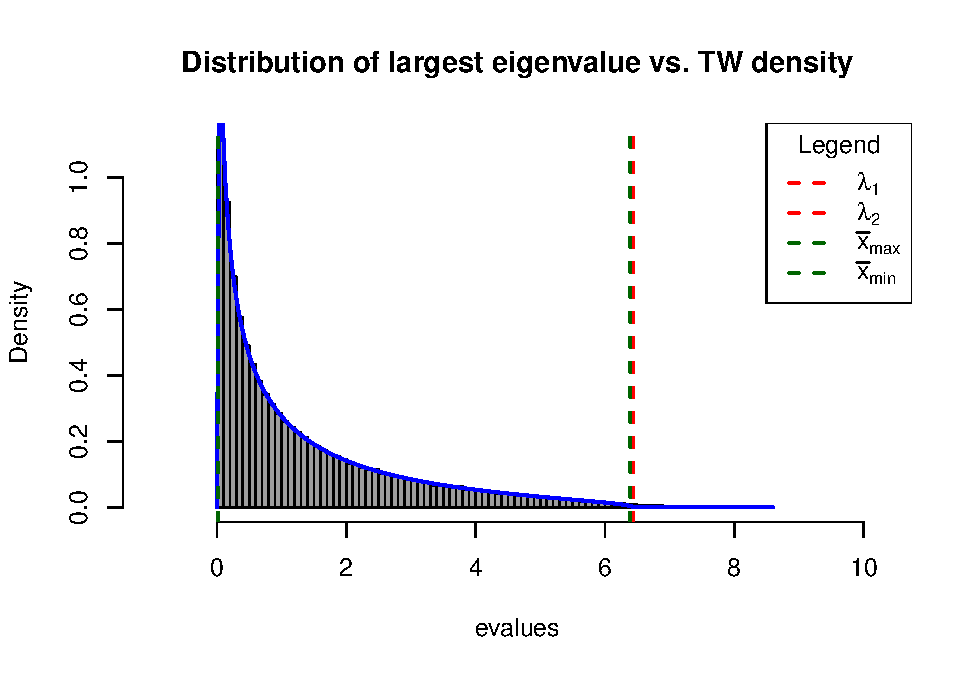
\includegraphics{A5_files/figure-latex/unnamed-chunk-9-1.pdf}

We can see that our simulated locations correspond well to expected
locations for \(\delta_1\) and for \(\delta_2\), respectively 6.43173
and 0.01728. We can see their values.

\begin{Shaded}
\begin{Highlighting}[]
\NormalTok{lambda\_1}
\end{Highlighting}
\end{Shaded}

\begin{verbatim}
## [1] 6.43173
\end{verbatim}

\begin{Shaded}
\begin{Highlighting}[]
\NormalTok{lambda\_2}
\end{Highlighting}
\end{Shaded}

\begin{verbatim}
## [1] 0.01728772
\end{verbatim}

\begin{Shaded}
\begin{Highlighting}[]
\FunctionTok{mean}\NormalTok{(eval\_max)}
\end{Highlighting}
\end{Shaded}

\begin{verbatim}
## [1] 6.391876
\end{verbatim}

\begin{Shaded}
\begin{Highlighting}[]
\FunctionTok{mean}\NormalTok{(eval\_min)}
\end{Highlighting}
\end{Shaded}

\begin{verbatim}
## [1] 0.01881308
\end{verbatim}

\begin{enumerate}
\def\labelenumi{(\alph{enumi})}
\setcounter{enumi}{5}
\tightlist
\item
  Consider the signal detection problem where we are trying to determine
  the number of signals in observations of the form
\end{enumerate}

\[
x_i = Us_i + \varepsilon_i, \quad i = 1, \ldots, m, \quad \text{(SD)}
\]

where the \(x_i\)'s are \(p\)-dimensional observations, \(s_i\) is a
\(k \times 1\) low dimensional signal (\(k \ll p\)) with covariance
\(I_k\), \(U\) is a \(p \times k\) mixing matrix, and
\((\varepsilon_i)\) is an i.i.d. noise with covariance matrix
\(\Sigma^2\). None of the quantities on the right hand side of (SD) are
observed. In Section 7.2 of {[}B{]}, they propose to estimate the number
of signals \(k\) by

\[
\hat{k} := \max\{i : \lambda_i \geq \beta + \log(p/p^{2/3})\},
\]

where \((\lambda_i)\) are the eigenvalues of \(\mathbf{S}\). Reproduce
Case 1 in Table 1 of {[}B{]} for the Gaussian case for values
\(p = 25, 75, 125, 175, 225, 275\). Fix \(y = 1/10\) and \(c = 9/10\),
further parameters and setup can be found at the bottom of p.436 and on
p.437.

\paragraph{\texorpdfstring{\textbf{Answer to question 1
(f)}:}{Answer to question 1 (f):}}\label{answer-to-question-1-f}

From the setup for Model 1 of {[}B{]}, we have that the
\(cov(\varepsilon_i) = diag(1,..,1, 2,,, 2)\) with \(p/2\) number of 1s
and 2s and given \(\varepsilon_i s\) are iid distributed and
\(cov(s_i) = I_k\) we have: \begin{align*}
\text{cov}(x_i) & = \text{cov}(U s_i + \varepsilon_i, U s_i + \varepsilon_i) \\& = \text{cov}(U s_i, U s_i) + 2\text{cov}(U s_i , \varepsilon_i) + \text{cov}(\varepsilon_i, \varepsilon_i) \\& = \text{cov}(U s_i, U s_i) + \text{cov}(\varepsilon_i, \varepsilon_i)\\& = (c_1\nu_1nu_1^T +  c_2\nu_2nu_2^T) + cov(\varepsilon_i)
\end{align*}

Also, it is easy to see that
\(c_1\nu_1 \nu_1^T + c_2\nu_2 \nu_2^T = diag(c_1, c_2, c_2, 0, ...,0) \in R^{p \times p}\)
in the paper setting. Now we normalized covariance matrix of \(x_i\) by
that of \(\varepsilon_i\), and then we have the following:
\begin{align*}
cov(x_i)*cov(\varepsilon_i)^{-1} = (c_1\nu_1nu_1^T +  c_2\nu_2nu_2^T)*cov(\varepsilon_i)^{-1} + I_p
\end{align*}

This is equal to a Fisher statistic with
\(\Sigma_1 = (c_1\nu_1nu_1^T + c_2\nu_2nu_2^T)*cov(\varepsilon_i)^{-1} + I_p\)
and \(Sigma_2 = I_p\). So the perturbation
\(\Delta = (c_1\nu_1nu_1^T + c_2\nu_2nu_2^T)*cov(\varepsilon_i)^{-1}\)
and \(\Sigma_1\) has eigenvalues \(c_1 + 1\) and \(c_2+1\) with
multiplicity of 1 and 2 respectively.

Let's do some simulation in Gaussian case assume the 0 mean and
normalized covariance (see above \(\Sigma_1, \Sigma_2\)) to show this:

\begin{Shaded}
\begin{Highlighting}[]
\NormalTok{p\_list }\OtherTok{=} \FunctionTok{c}\NormalTok{(}\DecValTok{25}\NormalTok{, }\DecValTok{75}\NormalTok{, }\DecValTok{125}\NormalTok{, }\DecValTok{175}\NormalTok{, }\DecValTok{225}\NormalTok{, }\DecValTok{275}\NormalTok{)}
\NormalTok{y }\OtherTok{=} \DecValTok{1}\SpecialCharTok{/}\DecValTok{10}
\NormalTok{c }\OtherTok{=} \DecValTok{9}\SpecialCharTok{/}\DecValTok{10}
\NormalTok{gamma }\OtherTok{=} \DecValTok{1}\SpecialCharTok{/}\NormalTok{(}\DecValTok{1} \SpecialCharTok{{-}}\NormalTok{ y)}
\NormalTok{h }\OtherTok{=} \FunctionTok{sqrt}\NormalTok{(c }\SpecialCharTok{+}\NormalTok{ y }\SpecialCharTok{{-}}\NormalTok{ c}\SpecialCharTok{*}\NormalTok{y)}
\NormalTok{b }\OtherTok{=}\NormalTok{ (}\DecValTok{1} \SpecialCharTok{+}\NormalTok{ h)}\SpecialCharTok{\^{}}\DecValTok{2}\SpecialCharTok{/}\NormalTok{(}\DecValTok{1} \SpecialCharTok{{-}}\NormalTok{ y)}\SpecialCharTok{\^{}}\DecValTok{2}
\NormalTok{critical\_value }\OtherTok{=}\NormalTok{ gamma}\SpecialCharTok{*}\NormalTok{(}\DecValTok{1} \SpecialCharTok{+}\NormalTok{ h)}
\NormalTok{c1 }\OtherTok{=} \DecValTok{10}
\NormalTok{c2 }\OtherTok{=} \DecValTok{5}

\NormalTok{sim.F.signal }\OtherTok{=} \ControlFlowTok{function}\NormalTok{(c1, c2, p, c, y, b, }\AttributeTok{n\_sims =} \DecValTok{1}\NormalTok{) \{}
\NormalTok{  n }\OtherTok{=}\NormalTok{ p}\SpecialCharTok{/}\NormalTok{y}
\NormalTok{  m }\OtherTok{=}\NormalTok{ p}\SpecialCharTok{/}\NormalTok{c}
\NormalTok{  k\_hat }\OtherTok{=} \FunctionTok{c}\NormalTok{()}
  \ControlFlowTok{for}\NormalTok{ (sim }\ControlFlowTok{in} \DecValTok{1}\SpecialCharTok{:}\NormalTok{n\_sims) \{}
\NormalTok{    Sigma1 }\OtherTok{=} \FunctionTok{diag}\NormalTok{(}\AttributeTok{x =} \FunctionTok{c}\NormalTok{(c1, c2, c2, }\FunctionTok{rep}\NormalTok{(}\DecValTok{0}\NormalTok{, p}\DecValTok{{-}3}\NormalTok{)), p) }\SpecialCharTok{+} \FunctionTok{diag}\NormalTok{(p)}
\NormalTok{    Sigma2 }\OtherTok{=} \FunctionTok{diag}\NormalTok{(p)}
\NormalTok{    mu }\OtherTok{=} \FunctionTok{rep}\NormalTok{(}\DecValTok{0}\NormalTok{, p)}
\NormalTok{    X }\OtherTok{=} \FunctionTok{rmvn}\NormalTok{(m}\SpecialCharTok{+}\DecValTok{1}\NormalTok{, mu, Sigma1)}
\NormalTok{    Z }\OtherTok{=} \FunctionTok{rmvn}\NormalTok{(n}\SpecialCharTok{+}\DecValTok{1}\NormalTok{, mu, Sigma2)}
\NormalTok{    S1 }\OtherTok{=} \FunctionTok{t}\NormalTok{(X) }\SpecialCharTok{\%*\%}\NormalTok{ (X)}\SpecialCharTok{/}\NormalTok{m}
\NormalTok{    S2 }\OtherTok{=} \FunctionTok{t}\NormalTok{(Z) }\SpecialCharTok{\%*\%}\NormalTok{ (Z)}\SpecialCharTok{/}\NormalTok{n}
\NormalTok{    FF }\OtherTok{=} \FunctionTok{solve}\NormalTok{(S2) }\SpecialCharTok{\%*\%}\NormalTok{ S1}
\NormalTok{    eval }\OtherTok{=} \FunctionTok{eigen}\NormalTok{(FF, }\AttributeTok{only.values =} \ConstantTok{TRUE}\NormalTok{)}\SpecialCharTok{$}\NormalTok{values}
\NormalTok{    k\_hat }\OtherTok{=} \FunctionTok{c}\NormalTok{(k\_hat, }\FunctionTok{sum}\NormalTok{(eval }\SpecialCharTok{\textgreater{}=}\NormalTok{ b }\SpecialCharTok{+}  \FunctionTok{log}\NormalTok{(p}\SpecialCharTok{/}\NormalTok{p}\SpecialCharTok{\^{}}\NormalTok{\{}\DecValTok{2}\SpecialCharTok{/}\DecValTok{3}\NormalTok{\})))}
\NormalTok{  \}}
\NormalTok{  k\_hat}
\NormalTok{\}}

\NormalTok{probability1 }\OtherTok{=} \FunctionTok{c}\NormalTok{()}
\NormalTok{probability2 }\OtherTok{=} \FunctionTok{c}\NormalTok{()}
\NormalTok{probability3 }\OtherTok{=} \FunctionTok{c}\NormalTok{()}
\NormalTok{probability4 }\OtherTok{=} \FunctionTok{c}\NormalTok{()}

\ControlFlowTok{for}\NormalTok{(i }\ControlFlowTok{in} \DecValTok{1}\SpecialCharTok{:}\FunctionTok{length}\NormalTok{(p\_list))\{}
\NormalTok{  k\_hat }\OtherTok{=} \FunctionTok{sim.F.signal}\NormalTok{(c1, c2, p\_list[i], c, y, b, }\AttributeTok{n\_sims =} \DecValTok{1000}\NormalTok{)}
\NormalTok{  probability1 }\OtherTok{=} \FunctionTok{c}\NormalTok{(probability1, }\FunctionTok{sum}\NormalTok{(k\_hat}\SpecialCharTok{==}\DecValTok{1}\NormalTok{)}\SpecialCharTok{/}\FunctionTok{length}\NormalTok{(k\_hat))}
\NormalTok{  probability2 }\OtherTok{=} \FunctionTok{c}\NormalTok{(probability2, }\FunctionTok{sum}\NormalTok{(k\_hat}\SpecialCharTok{==}\DecValTok{2}\NormalTok{)}\SpecialCharTok{/}\FunctionTok{length}\NormalTok{(k\_hat))}
\NormalTok{  probability3 }\OtherTok{=} \FunctionTok{c}\NormalTok{(probability3, }\FunctionTok{sum}\NormalTok{(k\_hat}\SpecialCharTok{==}\DecValTok{3}\NormalTok{)}\SpecialCharTok{/}\FunctionTok{length}\NormalTok{(k\_hat))}
\NormalTok{  probability4 }\OtherTok{=} \FunctionTok{c}\NormalTok{(probability4, }\FunctionTok{sum}\NormalTok{(k\_hat}\SpecialCharTok{==}\DecValTok{4}\NormalTok{)}\SpecialCharTok{/}\FunctionTok{length}\NormalTok{(k\_hat))}
\NormalTok{\}}
\end{Highlighting}
\end{Shaded}

Let's see our version of Table 1:

\begin{Shaded}
\begin{Highlighting}[]
\NormalTok{data }\OtherTok{\textless{}{-}} \FunctionTok{data.frame}\NormalTok{(}
  \AttributeTok{p =}\NormalTok{ p\_list,}
  \AttributeTok{n =}\NormalTok{ p\_list}\SpecialCharTok{/}\NormalTok{y,}
  \AttributeTok{m =}\NormalTok{ p\_list}\SpecialCharTok{/}\NormalTok{c,}
  \StringTok{\textasciigrave{}}\AttributeTok{k=1}\StringTok{\textasciigrave{}} \OtherTok{=}\NormalTok{ probability1,}
  \StringTok{\textasciigrave{}}\AttributeTok{k=2}\StringTok{\textasciigrave{}} \OtherTok{=}\NormalTok{ probability2,}
  \StringTok{\textasciigrave{}}\AttributeTok{k=3}\StringTok{\textasciigrave{}} \OtherTok{=}\NormalTok{ probability3,}
  \StringTok{\textasciigrave{}}\AttributeTok{k=4}\StringTok{\textasciigrave{}} \OtherTok{=}\NormalTok{ probability4}
\NormalTok{)}

\FunctionTok{kable}\NormalTok{(data, }\AttributeTok{format =} \StringTok{"html"}\NormalTok{, }\AttributeTok{caption =} \StringTok{"Frequency of our estimator in Model 1"}\NormalTok{, }\AttributeTok{align =} \StringTok{"c"}\NormalTok{)}
\end{Highlighting}
\end{Shaded}

Frequency of our estimator in Model 1

p

n

m

k.1

k.2

k.3

k.4

25

250

27.77778

0.026

0.488

0.486

0

75

750

83.33333

0.000

0.171

0.829

0

125

1250

138.88889

0.000

0.093

0.907

0

175

1750

194.44444

0.000

0.063

0.937

0

225

2250

250.00000

0.000

0.033

0.967

0

275

2750

305.55556

0.000

0.024

0.976

0

Immediately, I can see that the frequency increases as p gets larger,
which confirms the consistency of our estimator.

\begin{Shaded}
\begin{Highlighting}[]
\FunctionTok{rm}\NormalTok{(}\AttributeTok{list=}\FunctionTok{ls}\NormalTok{())}
\end{Highlighting}
\end{Shaded}

\subsection{Question 2}\label{question-2}

In this question, we shall consider high-dimensional sample covariance
matrices of data that is sampled from an elliptical distribution. We say
that a random vector \(\mathbf{x}\) with zero mean follows an elliptical
distribution if (and only if) it has the stochastic representation
\[ \mathbf{x} = \xi A \mathbf{u}, \quad (\star) \]where the matrix
\(A \in \mathbb{R}^{p \times p}\) is nonrandom and
\(\text{rank}(A) = p\), \(\xi \geq 0\) is a random variable representing
the radius of \(\mathbf{x}\), and \(u \in \mathbb{R}^p\) is the random
direction, which is independent of \(\xi\) and uniformly distributed on
the unit sphere \(S_{p-1}\) in \(\mathbb{R}^p\), denoted by
\(\mathbf{u} \sim \text{Unif}(S_{p-1})\). The class of elliptical
distributions is a natural generalization of the multivariate normal
distribution, and contains many widely used distributions as special
cases including the multivariate t-distribution, the symmetric
multivariate Laplace distribution, and the symmetric multivariate stable
distribution.

\begin{enumerate}
\def\labelenumi{(\alph{enumi})}
\tightlist
\item
  Write a function \texttt{runifsphere(n,p)} that samples \(n\)
  observations from the distribution \(\text{Unif}(S_{p-1})\) using the
  fact that if \(\mathbf{z} \sim N_p(0, I_p)\) then
  \(\frac{\mathbf{z}}{\| \mathbf{z} \|} \sim \text{Unif}(S_{p-1})\).
  Check your results by:
\end{enumerate}

\begin{enumerate}
\def\labelenumi{\arabic{enumi}.}
\tightlist
\item
  set \(p = 25\), \(n = 50\) and show that the (Euclidean) norm of each
  observation is equal to 1.
\end{enumerate}

\paragraph{\texorpdfstring{\textbf{Answer to question 2 (a)
(1)}:}{Answer to question 2 (a) (1):}}\label{answer-to-question-2-a-1}

Now we show that the (Euclidean) norm of each observation is equal to 1
in (1):

\begin{Shaded}
\begin{Highlighting}[]
\NormalTok{runifsphere }\OtherTok{\textless{}{-}} \ControlFlowTok{function}\NormalTok{(n, p) \{}
  \CommentTok{\# Generate n samples from N\_p(0, I\_p)}
\NormalTok{  mu }\OtherTok{=} \FunctionTok{rep}\NormalTok{(}\DecValTok{0}\NormalTok{, p)}
\NormalTok{  Sigma2 }\OtherTok{=} \FunctionTok{diag}\NormalTok{(p) }
\NormalTok{  z }\OtherTok{=} \FunctionTok{rmvn}\NormalTok{(n, mu, Sigma2)}

  
  \CommentTok{\# Normalize each sample to have unit norm}
\NormalTok{  norms }\OtherTok{\textless{}{-}} \FunctionTok{sqrt}\NormalTok{(}\FunctionTok{rowSums}\NormalTok{(z}\SpecialCharTok{\^{}}\DecValTok{2}\NormalTok{))}
\NormalTok{  samples\_on\_sphere }\OtherTok{\textless{}{-}} \FunctionTok{sweep}\NormalTok{(z, }\DecValTok{1}\NormalTok{, norms, }\AttributeTok{FUN =} \StringTok{"/"}\NormalTok{)}
  
  \FunctionTok{return}\NormalTok{(samples\_on\_sphere)}
\NormalTok{\}}

\NormalTok{p }\OtherTok{=} \DecValTok{25}
\NormalTok{n }\OtherTok{=} \DecValTok{50}
\NormalTok{u }\OtherTok{\textless{}{-}} \FunctionTok{runifsphere}\NormalTok{(n, p)}
\NormalTok{norms }\OtherTok{\textless{}{-}} \FunctionTok{sqrt}\NormalTok{(}\FunctionTok{rowSums}\NormalTok{(u}\SpecialCharTok{\^{}}\DecValTok{2}\NormalTok{))}
\NormalTok{norms}
\end{Highlighting}
\end{Shaded}

\begin{verbatim}
##  [1] 1 1 1 1 1 1 1 1 1 1 1 1 1 1 1 1 1 1 1 1 1 1 1 1 1 1 1 1 1 1 1 1 1 1 1 1 1 1
## [39] 1 1 1 1 1 1 1 1 1 1 1 1
\end{verbatim}

\begin{enumerate}
\def\labelenumi{(\arabic{enumi})}
\setcounter{enumi}{1}
\tightlist
\item
  generate a scatter plot in the case \(p = 2\), \(n = 500\) to show
  that the samples lie on a circle.
\end{enumerate}

\paragraph{\texorpdfstring{\textbf{Answer to question 2 (a)
(2)}:}{Answer to question 2 (a) (2):}}\label{answer-to-question-2-a-2}

Now we show that the observations lie on a circle in (2):

\begin{Shaded}
\begin{Highlighting}[]
\NormalTok{p }\OtherTok{=} \DecValTok{2}
\NormalTok{n }\OtherTok{=} \DecValTok{500}
\NormalTok{u2 }\OtherTok{\textless{}{-}} \FunctionTok{runifsphere}\NormalTok{(n, p)}

\CommentTok{\# Create a scatter plot of the samples}
\FunctionTok{plot}\NormalTok{(u2[,}\DecValTok{1}\NormalTok{], u2[,}\DecValTok{2}\NormalTok{], }\AttributeTok{xlim =} \FunctionTok{c}\NormalTok{(}\SpecialCharTok{{-}}\DecValTok{1}\NormalTok{, }\DecValTok{1}\NormalTok{), }\AttributeTok{ylim =} \FunctionTok{c}\NormalTok{(}\SpecialCharTok{{-}}\DecValTok{1}\NormalTok{, }\DecValTok{1}\NormalTok{), }\AttributeTok{xlab =} \StringTok{"X"}\NormalTok{, }\AttributeTok{ylab =} \StringTok{"Y"}\NormalTok{, }\AttributeTok{asp =} \DecValTok{1}\NormalTok{, }\AttributeTok{main =} \StringTok{"Samples from Unif(S1)"}\NormalTok{)}
\end{Highlighting}
\end{Shaded}

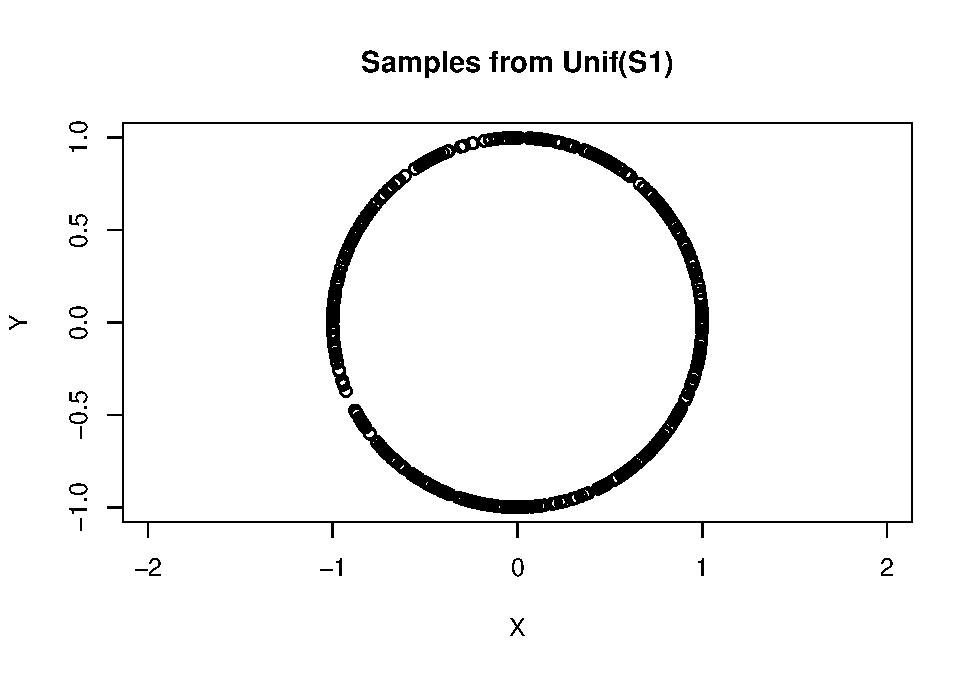
\includegraphics{A5_files/figure-latex/unnamed-chunk-15-1.pdf}

Show that you can simulate a multivariate \(p\) t-distribution
\(t_\nu(0, I_p)\) by setting \(\xi \sim \sqrt\frac{\nu}{C}\) in
\((\star)\) with \(A = I_p\) and \(C \sim \chi^2_\nu\). Do this by
sampling observations \(\mathbf{x}_1, \ldots, \mathbf{x}_n\) and
comparing the two marginal histograms of the observations against the
density of the univariate \(t_\nu\) distribution. Take \(p = 2\),
\(n = 1000\), \(\nu = 2\).

\paragraph{\texorpdfstring{\textbf{Answer to question 2 (a) part
3}:}{Answer to question 2 (a) part 3:}}\label{answer-to-question-2-a-part-3}

\begin{Shaded}
\begin{Highlighting}[]
\CommentTok{\# Parameters}
\NormalTok{p }\OtherTok{\textless{}{-}} \DecValTok{2}
\NormalTok{n }\OtherTok{\textless{}{-}} \DecValTok{1000}
\NormalTok{nu }\OtherTok{\textless{}{-}} \DecValTok{2}

\CommentTok{\# Simulate from multivariate t{-}distribution}
\NormalTok{rellipse\_t }\OtherTok{\textless{}{-}} \ControlFlowTok{function}\NormalTok{(n, p, nu) \{}
\NormalTok{  u }\OtherTok{\textless{}{-}} \FunctionTok{runifsphere}\NormalTok{(n, p)}
\NormalTok{  A }\OtherTok{=} \FunctionTok{diag}\NormalTok{(p)}
  
  \CommentTok{\# Generate xi}
\NormalTok{  C }\OtherTok{\textless{}{-}} \FunctionTok{rchisq}\NormalTok{(n, }\AttributeTok{df =}\NormalTok{ nu)}
\NormalTok{  xi }\OtherTok{\textless{}{-}} \FunctionTok{sqrt}\NormalTok{(nu }\SpecialCharTok{/}\NormalTok{ C)}
  
  \CommentTok{\# Compute x}
\NormalTok{  x }\OtherTok{\textless{}{-}}\NormalTok{ xi }\SpecialCharTok{*} \FunctionTok{t}\NormalTok{(A }\SpecialCharTok{\%*\%} \FunctionTok{t}\NormalTok{(u))}
  
  \FunctionTok{return}\NormalTok{(x)}
\NormalTok{\}}

\CommentTok{\# Generate samples}
\NormalTok{samples }\OtherTok{\textless{}{-}} \FunctionTok{rellipse\_t}\NormalTok{(n, p, nu)}

\CommentTok{\# Plot histograms against t{-}distribution density}
\FunctionTok{par}\NormalTok{(}\AttributeTok{mfrow =} \FunctionTok{c}\NormalTok{(}\DecValTok{1}\NormalTok{, }\DecValTok{2}\NormalTok{))}
\FunctionTok{hist}\NormalTok{(samples[,}\DecValTok{1}\NormalTok{], }\AttributeTok{breaks =} \DecValTok{40}\NormalTok{, }\AttributeTok{prob =} \ConstantTok{TRUE}\NormalTok{, }\AttributeTok{main =} \StringTok{"Histogram of x1"}\NormalTok{, }\AttributeTok{xlab =} \StringTok{"x1"}\NormalTok{)}
\FunctionTok{curve}\NormalTok{(}\FunctionTok{dt}\NormalTok{(x, }\AttributeTok{df =}\NormalTok{ nu), }\AttributeTok{col =} \StringTok{"red"}\NormalTok{, }\AttributeTok{lwd =} \DecValTok{2}\NormalTok{, }\AttributeTok{add =} \ConstantTok{TRUE}\NormalTok{)}
\FunctionTok{hist}\NormalTok{(samples[,}\DecValTok{2}\NormalTok{], }\AttributeTok{breaks =} \DecValTok{40}\NormalTok{, }\AttributeTok{prob =} \ConstantTok{TRUE}\NormalTok{, }\AttributeTok{main =} \StringTok{"Histogram of x2"}\NormalTok{, }\AttributeTok{xlab =} \StringTok{"x2"}\NormalTok{)}
\FunctionTok{curve}\NormalTok{(}\FunctionTok{dt}\NormalTok{(x, }\AttributeTok{df =}\NormalTok{ nu), }\AttributeTok{col =} \StringTok{"red"}\NormalTok{, }\AttributeTok{lwd =} \DecValTok{2}\NormalTok{, }\AttributeTok{add =} \ConstantTok{TRUE}\NormalTok{)}
\end{Highlighting}
\end{Shaded}

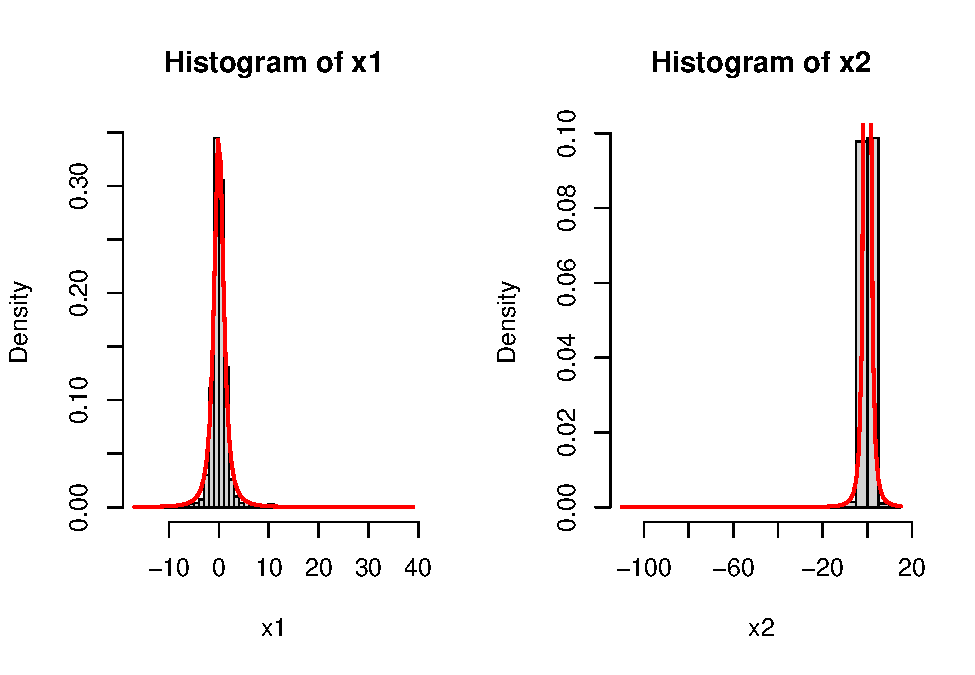
\includegraphics{A5_files/figure-latex/unnamed-chunk-16-1.pdf}

We can see that the plot matches the distribution very well.

\begin{enumerate}
\def\labelenumi{(\alph{enumi})}
\setcounter{enumi}{1}
\tightlist
\item
  Suppose that \(\mathbf{x}_1, \mathbf{x}_2, \dots, \mathbf{x}_n\) are
  \(p\)-dimensional observations sampled from an elliptic distribution
  \((\star)\). We stack these observations into the data matrix
  \(\mathbf{X}\) and calculate the sample covariance matrix
  \(\mathbf{S}_n := \mathbf{X} \mathbf{X}^T / n\). Theorem 2.2 of the
  recent paper {[}C{]} is a central limit theorem for linear spectral
  statistics (LSS) of \(\mathbf{S}_n\). For example, Eq. (2.10) in
  {[}C{]} provides the case of the joint distribution of the LSS
  \(\phi_1(x) = x\) and \(\phi_2(x) = x^2\). Following the notation used
  there (for all the following terms in this question). Perform a
  simulation experiment to examine the fluctuations of
  \(\hat{\beta}_{n1}\) and \(\hat{\beta}_{n2}\). In the experiment, take
  \(H_p = \frac{1}{2} \delta_1 + \frac{1}{2} \delta_2\) and choose the
  distribution of \(\xi \sim k_1 \text{Gamma}(p, 1)\) with
  \(k_1 = \frac{1}{\sqrt{p + 1}}\). Set the dimensions to be \(p = 200\)
  and \(n = 400\). Choose the number of simulations based on the
  computational power of your machine. Similar to Figure 1 in {[}C{]},
  use a QQ-plot to show normality.
\end{enumerate}

\paragraph{\texorpdfstring{\textbf{Answer to question 2
(b)}:}{Answer to question 2 (b):}}\label{answer-to-question-2-b}

The population \(PSD \ H_p\) is assumed to be fixed and therefore we
have \(H_p = H\). Immediately, we have the following conclusion:

\[
\gamma_{nj} = \int_{} t^jdH_p(t) = \int_{} t^jdH(t) = \gamma_j
\]

In this question, we assume that the
\(H_p = \frac{1}{2} \delta_1 + \frac{1}{2} \delta_2 \Rightarrow \Sigma = diag(1,..,1,2,...,2)=AA^T\)
with equal number of 1's and 2's so we can compute their respectively
values: \begin{align*}
\gamma_1 = \gamma_{n1} = \int t dH_p(t) = \int t d(\frac{1}{2}\delta_1 + \frac{1}{2}\delta_2) = \frac{1}{2} \int t d\delta_1(t) + \frac{1}{2} \int t d \delta_2(t) \\
\gamma_2 = \gamma_{n2} = \int t^2 dH_p(t) = \int t^2 d(\frac{1}{2}\delta_1 + \frac{1}{2}\delta_2) = \frac{1}{2} \int t^2 d\delta_1(t) + \frac{1}{2} \int t^2 d \delta_2(t)
\end{align*}

By propert \begin{equation*}
\int f(t) \delta_a(t)dt = f(a) \tag{1}
\end{equation*}

We have that: \begin{align*}
\int t d \delta_2(t) = 1\\
\int t d \delta_2(t) = 2\\
\int t^2 d\delta_1(t) = 1^2\\
\int t^2 d\delta_2(t) = 2^2\\
\end{align*}

\[
\gamma_1  = \gamma_{n1} = 1.5 \quad \text{and} \quad \gamma_2 = \gamma_{n2} =2.5 \quad \text{similarly} \quad \gamma_3 = 4.5 \quad \text{and} \quad \gamma_4 = 8.5
\]

The value we need to show the CLT assuming
\(p = 200, \quad n = 400 \quad \text{and} \quad \frac{p}{n} :=c_n = c = \frac{1}{2}\):
\begin{align*}
\tau & = 4\\
\beta_{n1} & = \gamma_{n1} = 1.5, \\
\beta_{n2} & = \gamma_{n2} + c_n\gamma^2_{n1} = 2.5 + \frac{1}{2} 1.5^2 = 3.625, \\
\nu_1 &= 0, \\
\nu_2 &= c\gamma_2 + c(\tau - 2)\gamma_1, \\
\psi_{11} & = 2c\gamma_2 + c(\tau - 2)\gamma^2_1 =  2.5 + 1.5^2 = 4.75, \\
\psi_{22} & = 8c\gamma_4 + 4c^2\gamma^2_2 + 16c^2\gamma_1\gamma_3 + 8c^3\gamma^2_1 \gamma_2 + 4c(\tau - 2)(c\gamma^2_1 + \gamma_2)^2 = 125.4375
\end{align*}

Let's code up these variables into R:

\begin{Shaded}
\begin{Highlighting}[]
\NormalTok{p }\OtherTok{=} \DecValTok{200}
\NormalTok{n }\OtherTok{=} \DecValTok{400}
\NormalTok{c }\OtherTok{=}\NormalTok{ p}\SpecialCharTok{/}\NormalTok{n}
\NormalTok{gamma\_1 }\OtherTok{=} \FloatTok{1.5}
\NormalTok{gamma\_2 }\OtherTok{=} \FloatTok{2.5}
\NormalTok{gamma\_3 }\OtherTok{=} \FloatTok{4.5}
\NormalTok{gamma\_4 }\OtherTok{=} \FloatTok{8.5}
\NormalTok{tau }\OtherTok{=} \DecValTok{4}
\NormalTok{beta\_n1 }\OtherTok{=}\NormalTok{ gamma\_1}
\NormalTok{beta\_n2 }\OtherTok{=}\NormalTok{ gamma\_2 }\SpecialCharTok{+}\NormalTok{ c}\SpecialCharTok{*}\NormalTok{gamma\_1}\SpecialCharTok{\^{}}\DecValTok{2}
\NormalTok{nu\_1 }\OtherTok{=} \DecValTok{0}
\NormalTok{nu\_2 }\OtherTok{=}\NormalTok{ c}\SpecialCharTok{*}\NormalTok{gamma\_2 }\SpecialCharTok{+}\NormalTok{ c}\SpecialCharTok{*}\NormalTok{(tau }\SpecialCharTok{{-}} \DecValTok{2}\NormalTok{)}\SpecialCharTok{*}\NormalTok{gamma\_1}
\NormalTok{psi\_11 }\OtherTok{=} \DecValTok{2} \SpecialCharTok{*}\NormalTok{ c }\SpecialCharTok{*}\NormalTok{ gamma\_2 }\SpecialCharTok{+}\NormalTok{ c }\SpecialCharTok{*}\NormalTok{ (tau }\SpecialCharTok{{-}} \DecValTok{2}\NormalTok{) }\SpecialCharTok{*}\NormalTok{ gamma\_1}\SpecialCharTok{\^{}} \DecValTok{2}
\NormalTok{psi\_22 }\OtherTok{=} \DecValTok{8}\SpecialCharTok{*}\NormalTok{c}\SpecialCharTok{*}\NormalTok{gamma\_4 }\SpecialCharTok{+} \DecValTok{4}\SpecialCharTok{*}\NormalTok{c}\SpecialCharTok{\^{}}\DecValTok{2}\SpecialCharTok{*}\NormalTok{gamma\_2}\SpecialCharTok{\^{}}\DecValTok{2} \SpecialCharTok{+} \DecValTok{16}\SpecialCharTok{*}\NormalTok{c}\SpecialCharTok{\^{}}\DecValTok{2}\SpecialCharTok{*}\NormalTok{gamma\_1}\SpecialCharTok{*}\NormalTok{gamma\_3 }\SpecialCharTok{+} \DecValTok{8}\SpecialCharTok{*}\NormalTok{c}\SpecialCharTok{\^{}}\DecValTok{3}\SpecialCharTok{*}\NormalTok{gamma\_1}\SpecialCharTok{\^{}}\DecValTok{2}\SpecialCharTok{*}\NormalTok{gamma\_2 }\SpecialCharTok{+} \DecValTok{4}\SpecialCharTok{*}\NormalTok{c}\SpecialCharTok{*}\NormalTok{(tau }\SpecialCharTok{{-}} \DecValTok{2}\NormalTok{)}\SpecialCharTok{*}\NormalTok{(c}\SpecialCharTok{*}\NormalTok{gamma\_1}\SpecialCharTok{\^{}}\DecValTok{2} \SpecialCharTok{+}\NormalTok{ gamma\_2)}\SpecialCharTok{\^{}}\DecValTok{2}
\end{Highlighting}
\end{Shaded}

To facilitate our simulation later, we will construct a function that
can generate the ellipse distribution under the question setting:

\begin{Shaded}
\begin{Highlighting}[]
\NormalTok{rellipse }\OtherTok{\textless{}{-}} \ControlFlowTok{function}\NormalTok{(n, p)\{}
\NormalTok{  u }\OtherTok{\textless{}{-}} \FunctionTok{runifsphere}\NormalTok{(n, p)}
  \CommentTok{\# A = diag(x = c(rep(1, p/2), rep(2, p/2)), p)}
  \ControlFlowTok{if}\NormalTok{(p }\SpecialCharTok{\%\%} \DecValTok{2} \SpecialCharTok{==} \DecValTok{0}\NormalTok{)\{}
\NormalTok{    A }\OtherTok{=} \FunctionTok{diag}\NormalTok{(}\AttributeTok{x =} \FunctionTok{c}\NormalTok{(}\FunctionTok{rep}\NormalTok{(}\DecValTok{1}\NormalTok{, p}\SpecialCharTok{/}\DecValTok{2}\NormalTok{), }\FunctionTok{rep}\NormalTok{(}\FunctionTok{sqrt}\NormalTok{(}\DecValTok{2}\NormalTok{), p}\SpecialCharTok{/}\DecValTok{2}\NormalTok{)), p)}
\NormalTok{  \}}\ControlFlowTok{else}\NormalTok{\{}
\NormalTok{    A }\OtherTok{=} \FunctionTok{diag}\NormalTok{(}\AttributeTok{x =} \FunctionTok{c}\NormalTok{(}\FunctionTok{rep}\NormalTok{(}\DecValTok{1}\NormalTok{, }\FunctionTok{floor}\NormalTok{(p}\SpecialCharTok{/}\DecValTok{2}\NormalTok{)), }\FunctionTok{rep}\NormalTok{(}\FunctionTok{sqrt}\NormalTok{(}\DecValTok{2}\NormalTok{), p }\SpecialCharTok{{-}} \FunctionTok{floor}\NormalTok{(p}\SpecialCharTok{/}\DecValTok{2}\NormalTok{))), p)}
\NormalTok{  \}}
  
  \CommentTok{\# Generate xi}
\NormalTok{  k\_1 }\OtherTok{=} \DecValTok{1}\SpecialCharTok{/}\FunctionTok{sqrt}\NormalTok{(p}\SpecialCharTok{+}\DecValTok{1}\NormalTok{)}
\NormalTok{  xi }\OtherTok{\textless{}{-}}\NormalTok{ k\_1 }\SpecialCharTok{*} \FunctionTok{rgamma}\NormalTok{(n, }\AttributeTok{shape =}\NormalTok{ p , }\AttributeTok{scale =} \DecValTok{1}\NormalTok{)}

  \CommentTok{\# Compute x}
\NormalTok{  x }\OtherTok{\textless{}{-}}\NormalTok{ xi }\SpecialCharTok{*} \FunctionTok{t}\NormalTok{(A }\SpecialCharTok{\%*\%} \FunctionTok{t}\NormalTok{(u))}
  
  \FunctionTok{return}\NormalTok{(x)}
\NormalTok{\}}
\end{Highlighting}
\end{Shaded}

Now, Let's simulate the fluctuations of \(\hat\beta_{n1}\), which
corresponds to the case where \(f(x) = x\) as defined above.

\begin{Shaded}
\begin{Highlighting}[]
\FunctionTok{plan}\NormalTok{(multisession, }\AttributeTok{workers =} \DecValTok{8}\NormalTok{)}
\NormalTok{n\_sims }\OtherTok{=} \DecValTok{5000}
\NormalTok{beta\_n1\_hat }\OtherTok{=} \FunctionTok{future\_replicate}\NormalTok{(n\_sims, \{}
\NormalTok{  p }\OtherTok{=} \DecValTok{200}
\NormalTok{  n }\OtherTok{=} \DecValTok{400}
\NormalTok{  X }\OtherTok{=} \FunctionTok{rellipse}\NormalTok{(n, p)}
\NormalTok{  Sn }\OtherTok{=} \FunctionTok{cov}\NormalTok{(X)}
\NormalTok{  L}\OtherTok{=}\FunctionTok{eigen}\NormalTok{(Sn, }\AttributeTok{only.values =} \ConstantTok{TRUE}\NormalTok{)}\SpecialCharTok{$}\NormalTok{values}
  \FunctionTok{sum}\NormalTok{(L)}\SpecialCharTok{/}\NormalTok{p}
\NormalTok{\})}
\NormalTok{LLS\_normalized }\OtherTok{=}\NormalTok{ p}\SpecialCharTok{*}\NormalTok{(beta\_n1\_hat }\SpecialCharTok{{-}}\NormalTok{ beta\_n1)}\SpecialCharTok{/}\FunctionTok{sqrt}\NormalTok{(psi\_11)}
\end{Highlighting}
\end{Shaded}

\begin{Shaded}
\begin{Highlighting}[]
\FunctionTok{qqnorm}\NormalTok{(LLS\_normalized, }\AttributeTok{main =} \StringTok{"QQ{-}Plot of LLS against N(0,1)"}\NormalTok{, }\AttributeTok{ylab =} \StringTok{"Quantiles of LLS"}\NormalTok{, }\AttributeTok{xlab =} \StringTok{"Quantiles of N(0,1)"}\NormalTok{)}
\FunctionTok{qqline}\NormalTok{(LLS\_normalized, }\AttributeTok{col =} \StringTok{"red"}\NormalTok{, }\AttributeTok{lwd =} \DecValTok{2}\NormalTok{)}
\end{Highlighting}
\end{Shaded}

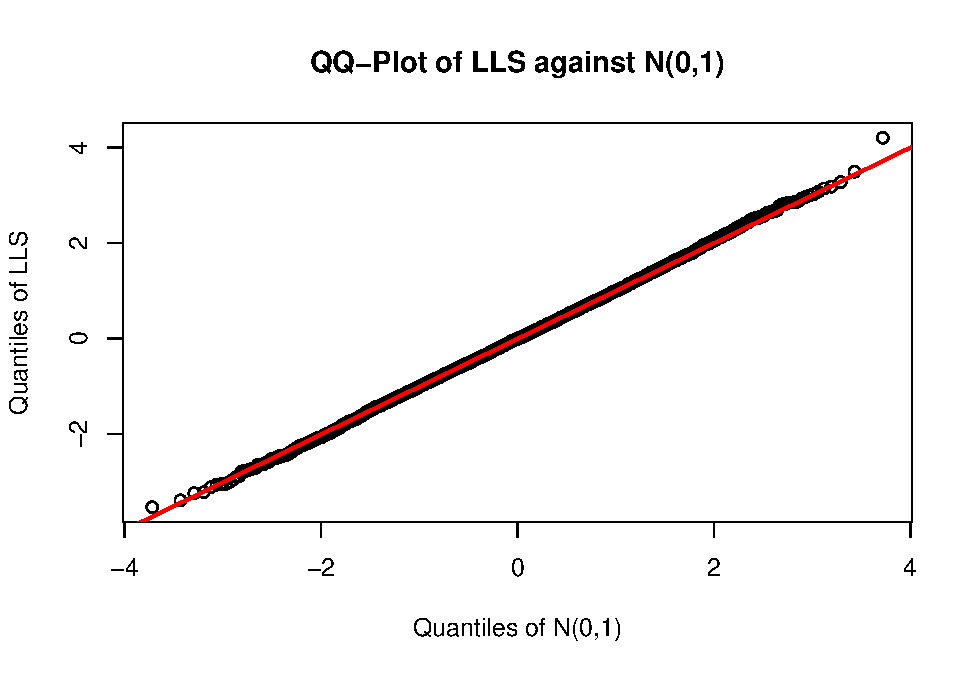
\includegraphics{A5_files/figure-latex/unnamed-chunk-20-1.pdf}

Now, Let's simulate the fluctuations of \(\hat\beta_{n2}\), which
corresponds to the case where \(f(x) = x^2\) as defined above.

\begin{Shaded}
\begin{Highlighting}[]
\NormalTok{n\_sims }\OtherTok{=} \DecValTok{5000}
\NormalTok{beta\_n2\_hat }\OtherTok{=} \FunctionTok{future\_replicate}\NormalTok{(n\_sims, \{}
\NormalTok{  p }\OtherTok{=} \DecValTok{200}
\NormalTok{  n }\OtherTok{=} \DecValTok{400}
\NormalTok{  X }\OtherTok{=} \FunctionTok{rellipse}\NormalTok{(n, p)}
\NormalTok{  Sn }\OtherTok{=} \FunctionTok{cov}\NormalTok{(X)}
\NormalTok{  L}\OtherTok{=}\FunctionTok{eigen}\NormalTok{(Sn, }\AttributeTok{only.values =} \ConstantTok{TRUE}\NormalTok{)}\SpecialCharTok{$}\NormalTok{values}
  \FunctionTok{sum}\NormalTok{(L}\SpecialCharTok{\^{}}\DecValTok{2}\NormalTok{)}\SpecialCharTok{/}\NormalTok{p}
\NormalTok{\})}
\NormalTok{LLS\_normalized }\OtherTok{=}\NormalTok{ ((p}\SpecialCharTok{*}\NormalTok{(beta\_n2\_hat }\SpecialCharTok{{-}}\NormalTok{ beta\_n2)) }\SpecialCharTok{{-}}\NormalTok{ nu\_2)}\SpecialCharTok{/}\FunctionTok{sqrt}\NormalTok{(psi\_22)}
\end{Highlighting}
\end{Shaded}

\begin{Shaded}
\begin{Highlighting}[]
\FunctionTok{qqnorm}\NormalTok{(LLS\_normalized, }\AttributeTok{main =} \StringTok{"QQ{-}Plot of LLS against N(0,1)"}\NormalTok{, }\AttributeTok{ylab =} \StringTok{"Quantiles of LLS"}\NormalTok{, }\AttributeTok{xlab =} \StringTok{"Quantiles of N(0,1)"}\NormalTok{)}
\FunctionTok{qqline}\NormalTok{(LLS\_normalized, }\AttributeTok{col =} \StringTok{"red"}\NormalTok{, }\AttributeTok{lwd =} \DecValTok{2}\NormalTok{)}
\end{Highlighting}
\end{Shaded}

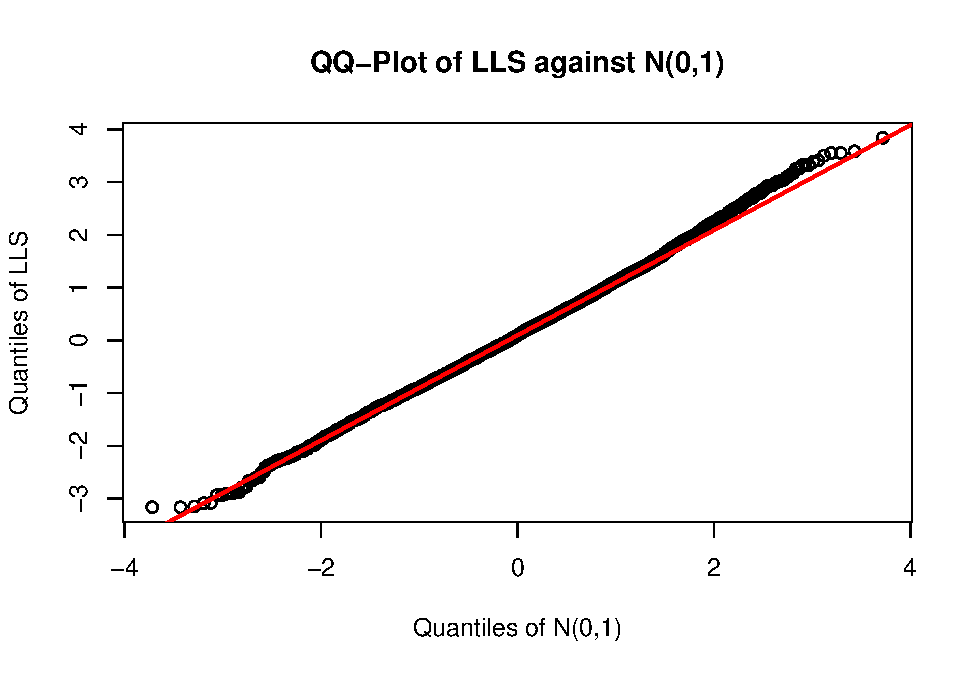
\includegraphics{A5_files/figure-latex/unnamed-chunk-22-1.pdf}

We can see that the linear spectral statistic (LSS) corresponds very
well to the standard normal distribution, and only shows occansionally
off at the tail.

\begin{enumerate}
\def\labelenumi{(\alph{enumi})}
\setcounter{enumi}{2}
\tightlist
\item
  In the recent paper {[}E{]}, it is shown that if
  \(\mathbf{x}_1, \mathbf{x}_2, \ldots, \mathbf{x}_n\) are
  \(p\)-dimensional observations sampled from an elliptic distribution
  (\(\star\)) then the largest eigenvalue \(\lambda_1\) of the sample
  covariance \(\mathbf{S}_n\) (appropriately scaled) converges to the
  Tracy-Widom distribution as long as a certain condition on the tail of
  the distribution holds (Condition 2.7 in the paper). Perform a
  simulation to show that this holds true in the case of a double
  exponential distribution but not in the case of a multivariate
  student-t distribution. That is, simulate the largest eigenvalue of
  the sample covariance matrix and compare it to the Tracy-Widom
  distribution in each case. In the first case it should match (double
  exponential) and in the second case it shouldn't (multivariate
  student-t).
\end{enumerate}

\paragraph{\texorpdfstring{\textbf{Answer to question 2
(c)}:}{Answer to question 2 (c):}}\label{answer-to-question-2-c}

Firstly, let's follow the above assumption \(A = I_p\). By making this
critical assumption, we achieve \(\Sigma = AA^T = I_p\) and thus the
population spectral distribution (PSD) \(H_p\) of matrix \(\Sigma\)
converge to the Dirac measure at 1, namely \(H(t) = \delta_1(t)\). By
Theorem 2.1 of {[}C{]}, we have that the emperical spectual distribution
of \(F^{S_n}\) , with \(S_n = \frac{1}{n}XX^T\in R^{p \times p}\)
converge weakly to the \(F^{c,H}\), which is a (not the general case of)
Marcenko-Pastur distributions with variance 1.

Thus, immediately we get that the upper end points of this distribution,
denoted as \(\lambda_+\) is
\(\lambda_+ = (1 + \sqrt c )^2, \quad where \ c = p/n\). Thus, by Claim
1 and Corollary 3.3 in {[}E{]}, we have
\(\gamma n^{2/3}(\lambda_1(B_n) - \lambda_+)\) should distribute as a
Tracy-Widom distribution. Firstly, let's consider the \(\gamma\).

\[
\frac{1}{\gamma^3} = \frac{1}{x^3} \left(1 + c\int (\frac{\lambda x}{1 - \lambda x})^3  \pi(d\lambda)\right)
\]

When we suppose that we have the PSD equal to \(\delta_1(t)\). By
property (1) (see above), this formula simplifies to:

\[
\gamma = \left(\frac{1}{x^3} + \frac{c}{(1-x)^3} \right)^{-\frac{1}{3}}
\]

From equation 2.9 in the paper {[}E{]}, we define \(f\) and the
relational formula between \(\lambda\) and \(x\): \(\lambda_+ := f(−x)\)

\[
f(x) := -\frac{1}{x} + c \int \frac{w\pi(dw)}{1 + wx}
\]

By property (1) (see above), this function simplifies to:

\[
f(-x) = \frac{1}{x} + c \frac{1}{1-x} = \lambda_+
\]

The first derivative and by 2.9 in {[}E{]}:

\[
f'(-x) = \frac{1}{x^2} - \frac{c}{(1-x)^2} = 0
\]

We get that:

\[
x_1 = \frac{1}{1-\sqrt c}, \quad x_2 = \frac{1}{1+\sqrt c}
\]

for \(x_1, x_2 \in (0, \sigma_1^{-1})\). The \(\sigma_1\) is the largest
eigenvalue in matrix \(\Sigma = I_p\) in our case so \(\sigma_1 = 1\).
When \(c=\frac{1}{2}\), we choose \(x_2\) to be the valid \(x\) in our
case.

Moreover, we will need \(\xi\) to satisfy the condition 2.7 in {[}E{]}.
It part (b), we see that the setting \(\xi \sim k_1 \text{Gamma}(p, 1)\)
and \(k_1 = \frac{1}{\sqrt{p + 1}}\) is the same as the condition 2.7.
We proof a little bit here:

\[
\lim_{s \to \infty} \limsup_{N \to \infty} s^2 P\left(|\hat{\xi}^2_i - M| > \sqrt{Ms}\right) = 0, \ \xi_i^2 = \hat\xi_i^2/ \sqrt N
\]

The \(\hat\xi_i^2\) is in our case \(\xi_i^2\). This generally says that
the \(\hat\xi_i^2\) should be closed to \(M\), which is \(p\) in our
notation. Also, condition 2.7 also says that \(E\xi_i^2 = \phi\). Let's
substitute the \(\xi_i^2 = \hat\xi_i^2/ \sqrt N\) and get
\(E\frac{\hat\xi_i}{N}^2 = \phi\) and it is the same as
\(E{\hat\xi_i}^2 = \phi*N = M\), which is equal to \(E{\xi_i}^2 = p\) in
{[}c{]}. This condition has been check when in part (b).

Let's write some codes to show this result. Firstly, let's show the case
where x follows double exponential distribution. This is to say
\(\xi \sim k_1 \text{Gamma}(p, 1)\) and \(k_1 = \frac{1}{\sqrt{p + 1}}\)
(to satisfy condition 2.7).

\begin{Shaded}
\begin{Highlighting}[]
\NormalTok{rellipse }\OtherTok{\textless{}{-}} \ControlFlowTok{function}\NormalTok{(n, p)\{}
\NormalTok{  u }\OtherTok{\textless{}{-}} \FunctionTok{runifsphere}\NormalTok{(n, p)}
\NormalTok{  A }\OtherTok{=} \FunctionTok{diag}\NormalTok{(p)}
  
  \CommentTok{\# Generate xi}
\NormalTok{  k\_1 }\OtherTok{=} \DecValTok{1}\SpecialCharTok{/}\FunctionTok{sqrt}\NormalTok{(p}\SpecialCharTok{+}\DecValTok{1}\NormalTok{)}
\NormalTok{  xi }\OtherTok{\textless{}{-}}\NormalTok{ k\_1 }\SpecialCharTok{*} \FunctionTok{rgamma}\NormalTok{(n, }\AttributeTok{shape =}\NormalTok{ p , }\AttributeTok{scale =} \DecValTok{1}\NormalTok{)}

  \CommentTok{\# Compute x}
\NormalTok{  x }\OtherTok{\textless{}{-}}\NormalTok{ xi }\SpecialCharTok{*} \FunctionTok{t}\NormalTok{(A }\SpecialCharTok{\%*\%} \FunctionTok{t}\NormalTok{(u))}
  
  \FunctionTok{return}\NormalTok{(x)}
\NormalTok{\}}

\NormalTok{n\_sims }\OtherTok{=} \DecValTok{1000}
\NormalTok{lambda\_1 }\OtherTok{=} \FunctionTok{future\_replicate}\NormalTok{(n\_sims, \{}
\NormalTok{  p }\OtherTok{=} \DecValTok{200}
\NormalTok{  n }\OtherTok{=} \DecValTok{400}
\NormalTok{  X }\OtherTok{=} \FunctionTok{rellipse}\NormalTok{(n, p)}
\NormalTok{  Sn }\OtherTok{=}\NormalTok{ X }\SpecialCharTok{\%*\%} \FunctionTok{t}\NormalTok{(X)}\SpecialCharTok{/}\NormalTok{n}
\NormalTok{  L}\OtherTok{=}\FunctionTok{eigen}\NormalTok{(Sn, }\AttributeTok{only.values =} \ConstantTok{TRUE}\NormalTok{)}\SpecialCharTok{$}\NormalTok{values}
  \FunctionTok{max}\NormalTok{(L)}
\NormalTok{\})}

\NormalTok{lambda\_plus }\OtherTok{=}\NormalTok{ (}\DecValTok{1} \SpecialCharTok{+} \FunctionTok{sqrt}\NormalTok{(c))}\SpecialCharTok{\^{}}\DecValTok{2}
\NormalTok{x }\OtherTok{=} \DecValTok{1}\SpecialCharTok{/}\NormalTok{(}\DecValTok{1}\SpecialCharTok{+}\FunctionTok{sqrt}\NormalTok{(c))}
\NormalTok{gamma }\OtherTok{=}\NormalTok{ (}\DecValTok{1}\SpecialCharTok{/}\NormalTok{x}\SpecialCharTok{\^{}}\DecValTok{3} \SpecialCharTok{+}\NormalTok{ c}\SpecialCharTok{/}\NormalTok{(}\DecValTok{1} \SpecialCharTok{{-}}\NormalTok{ x)}\SpecialCharTok{\^{}}\DecValTok{3}\NormalTok{)}\SpecialCharTok{\^{}}\NormalTok{\{}\SpecialCharTok{{-}}\DecValTok{1}\SpecialCharTok{/}\DecValTok{3}\NormalTok{\}}
\NormalTok{lambda\_normalized }\OtherTok{=}\NormalTok{ gamma}\SpecialCharTok{*}\NormalTok{n}\SpecialCharTok{\^{}}\NormalTok{\{}\DecValTok{2}\SpecialCharTok{/}\DecValTok{3}\NormalTok{\}}\SpecialCharTok{*}\NormalTok{(lambda\_1 }\SpecialCharTok{{-}}\NormalTok{ lambda\_plus)}
\end{Highlighting}
\end{Shaded}

\begin{Shaded}
\begin{Highlighting}[]
\NormalTok{h }\OtherTok{\textless{}{-}} \FunctionTok{hist}\NormalTok{(lambda\_normalized, }\AttributeTok{breaks=}\DecValTok{100}\NormalTok{, }\AttributeTok{freq =} \ConstantTok{FALSE}\NormalTok{, }\AttributeTok{xlim=}\FunctionTok{c}\NormalTok{(}\SpecialCharTok{{-}}\DecValTok{10}\NormalTok{,}\DecValTok{10}\NormalTok{))}
\end{Highlighting}
\end{Shaded}

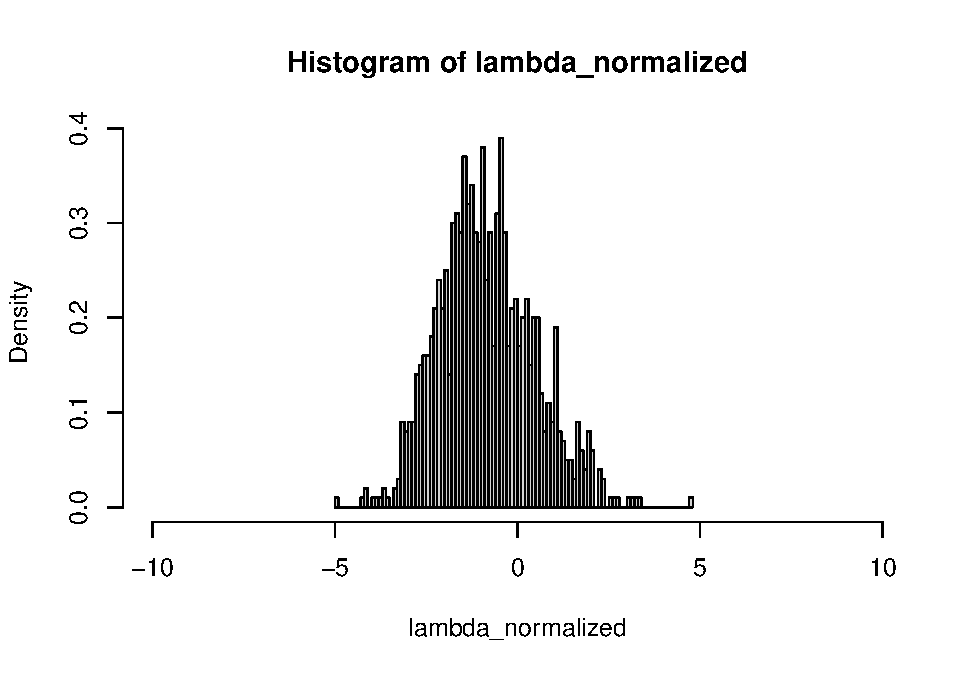
\includegraphics{A5_files/figure-latex/unnamed-chunk-24-1.pdf}

\begin{Shaded}
\begin{Highlighting}[]
\FunctionTok{plot}\NormalTok{(h}\SpecialCharTok{$}\NormalTok{mids, h}\SpecialCharTok{$}\NormalTok{density, }\AttributeTok{type=}\StringTok{"s"}\NormalTok{, }\AttributeTok{xlab=}\StringTok{""}\NormalTok{, }\AttributeTok{ylab=}\StringTok{""}\NormalTok{, }\AttributeTok{ylim=}\FunctionTok{c}\NormalTok{(}\DecValTok{0}\NormalTok{,}\DecValTok{1}\NormalTok{))}
\FunctionTok{curve}\NormalTok{(dtw, }\SpecialCharTok{{-}}\DecValTok{10}\NormalTok{, }\DecValTok{10}\NormalTok{, }\AttributeTok{lwd=}\DecValTok{2}\NormalTok{, }\AttributeTok{lty=}\DecValTok{3}\NormalTok{, }\AttributeTok{col=}\StringTok{"darkmagenta"}\NormalTok{, }\AttributeTok{add=}\ConstantTok{TRUE}\NormalTok{)}
\FunctionTok{title}\NormalTok{(}\AttributeTok{main=}\StringTok{"Distribution of largest eigenvalue vs. TW density"}\NormalTok{)}
\end{Highlighting}
\end{Shaded}

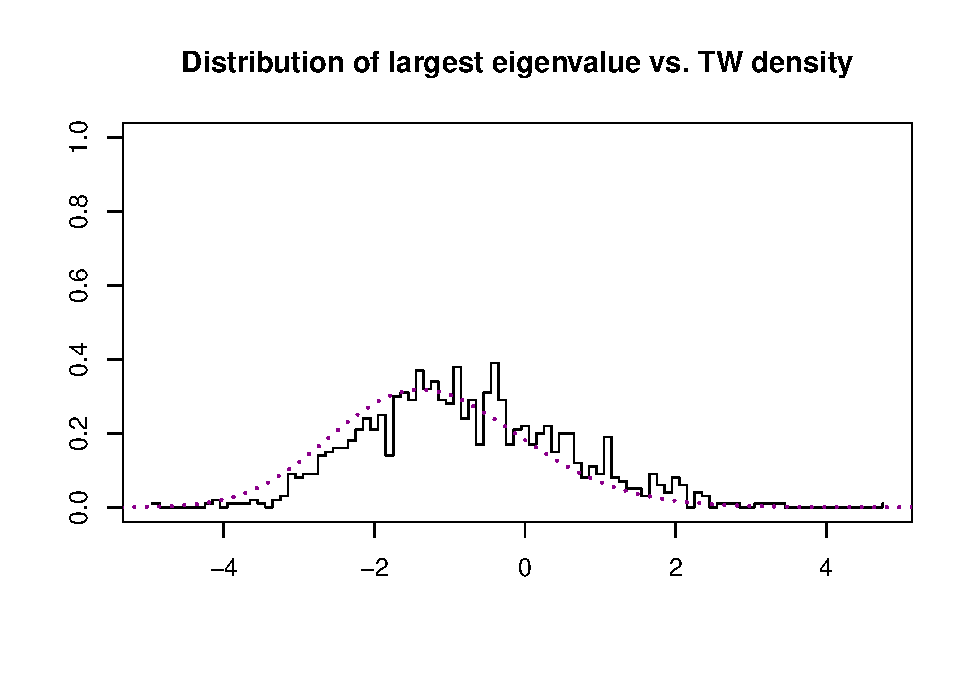
\includegraphics{A5_files/figure-latex/unnamed-chunk-24-2.pdf}

The above case follows the Tracy-Widom distribution well enough.
Secondly, let's show the case where x follows multivariate \(t\)
distribution.

\begin{Shaded}
\begin{Highlighting}[]
\NormalTok{rellipse }\OtherTok{\textless{}{-}} \ControlFlowTok{function}\NormalTok{(n, p, nu)\{}
\NormalTok{  u }\OtherTok{\textless{}{-}} \FunctionTok{runifsphere}\NormalTok{(n, p)}
\NormalTok{  A }\OtherTok{=} \FunctionTok{diag}\NormalTok{(p)}
  
  \CommentTok{\# Generate xi}
\NormalTok{  xi }\OtherTok{\textless{}{-}}\NormalTok{ p}\SpecialCharTok{*}\FunctionTok{rf}\NormalTok{(n, p, nu)}

  \CommentTok{\# Compute x}
\NormalTok{  x }\OtherTok{\textless{}{-}}\NormalTok{ xi }\SpecialCharTok{*} \FunctionTok{t}\NormalTok{(A }\SpecialCharTok{\%*\%} \FunctionTok{t}\NormalTok{(u))}
  
  \FunctionTok{return}\NormalTok{(x)}
\NormalTok{\}}

\NormalTok{n\_sims }\OtherTok{=} \DecValTok{1000}
\NormalTok{lambda\_1 }\OtherTok{=} \FunctionTok{future\_replicate}\NormalTok{(n\_sims, \{}
\NormalTok{  p }\OtherTok{=} \DecValTok{200}
\NormalTok{  n }\OtherTok{=} \DecValTok{400}
\NormalTok{  X }\OtherTok{=} \FunctionTok{rellipse}\NormalTok{(n, p, }\AttributeTok{nu =} \DecValTok{10}\NormalTok{)}
\NormalTok{  Sn }\OtherTok{=} \FunctionTok{cov}\NormalTok{(X)}
\NormalTok{  L}\OtherTok{=}\FunctionTok{eigen}\NormalTok{(Sn, }\AttributeTok{only.values =} \ConstantTok{TRUE}\NormalTok{)}\SpecialCharTok{$}\NormalTok{values}
  \FunctionTok{max}\NormalTok{(L)}
\NormalTok{\})}

\NormalTok{lambda\_plus }\OtherTok{=}\NormalTok{ (}\DecValTok{1} \SpecialCharTok{+} \FunctionTok{sqrt}\NormalTok{(c))}\SpecialCharTok{\^{}}\DecValTok{2}
\NormalTok{x }\OtherTok{=} \DecValTok{1}\SpecialCharTok{/}\NormalTok{(}\DecValTok{1}\SpecialCharTok{+}\FunctionTok{sqrt}\NormalTok{(c))}
\NormalTok{gamma }\OtherTok{=}\NormalTok{ (}\DecValTok{1}\SpecialCharTok{/}\NormalTok{x}\SpecialCharTok{\^{}}\DecValTok{3} \SpecialCharTok{+}\NormalTok{ c}\SpecialCharTok{/}\NormalTok{(}\DecValTok{1} \SpecialCharTok{{-}}\NormalTok{ x)}\SpecialCharTok{\^{}}\DecValTok{3}\NormalTok{)}\SpecialCharTok{\^{}}\NormalTok{\{}\SpecialCharTok{{-}}\DecValTok{1}\SpecialCharTok{/}\DecValTok{3}\NormalTok{\}}
\NormalTok{lambda\_normalized }\OtherTok{=}\NormalTok{ gamma}\SpecialCharTok{*}\NormalTok{n}\SpecialCharTok{\^{}}\NormalTok{\{}\DecValTok{2}\SpecialCharTok{/}\DecValTok{3}\NormalTok{\}}\SpecialCharTok{*}\NormalTok{(lambda\_1 }\SpecialCharTok{{-}}\NormalTok{ lambda\_plus)}
\end{Highlighting}
\end{Shaded}

\begin{Shaded}
\begin{Highlighting}[]
\FunctionTok{hist}\NormalTok{(lambda\_normalized, }\AttributeTok{breaks=}\DecValTok{80}\NormalTok{, }\AttributeTok{freq =} \ConstantTok{FALSE}\NormalTok{)}
\end{Highlighting}
\end{Shaded}

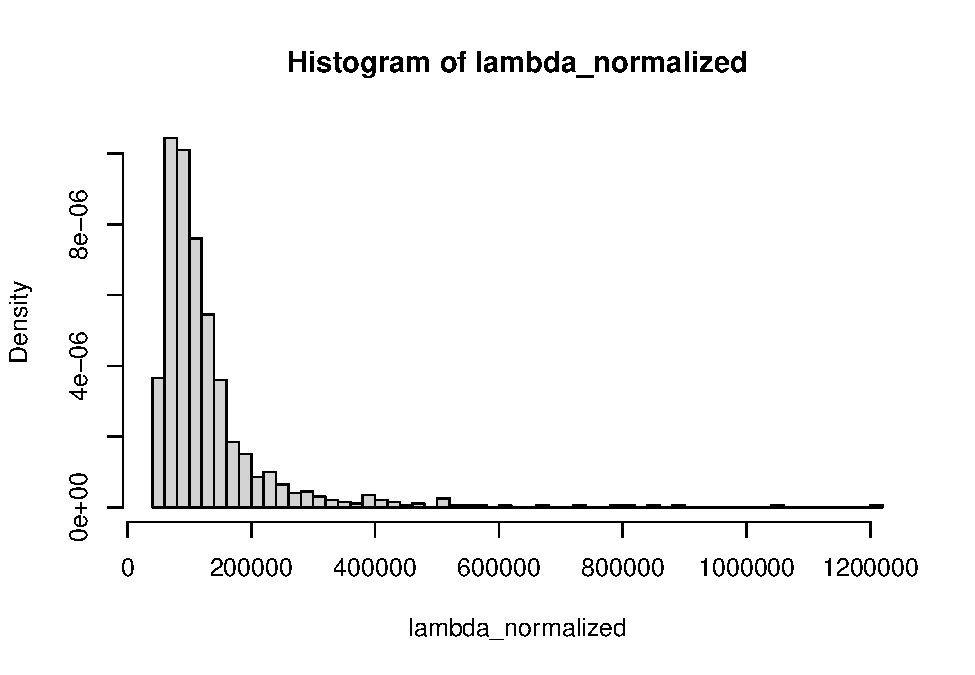
\includegraphics{A5_files/figure-latex/unnamed-chunk-26-1.pdf}

\begin{Shaded}
\begin{Highlighting}[]
\CommentTok{\# plot(h$mids, h$density, type="s", xlab="", ylab="", ylim=c(0,1))}
\CommentTok{\# curve(dtw, {-}10, 10, lwd=2, lty=3, col="darkmagenta", add=TRUE)}
\CommentTok{\# title(main="Distribution of largest eigenvalue vs. TW density")}
\end{Highlighting}
\end{Shaded}

We can see that this histogram does not follow the Tracy-Widom
distribution even in the normalized case.

\begin{enumerate}
\def\labelenumi{(\alph{enumi})}
\setcounter{enumi}{3}
\tightlist
\item
  A nice property of elliptic distributions \((\star)\) is that the
  mixture coefficient \(\xi\) can feature heteroskedasticity and the
  overall distribution of \(\mathbf{x}\) can exhibit heavy tails. Both
  are properties that are widely observed in financial and economic
  data, for example. In the recent paper {[}F{]}, they proposed a more
  generalized setting whereby the observations
\end{enumerate}

\[
\mathbf{x}_i = \xi_iA\mathbf{u}_i, \quad i = 1, \ldots, n.
\]

may exhibit the situation that

\begin{itemize}
\tightlist
\item
  \(\xi_i\)'s can depend on each other and on
  \(\{ \mathbf{u}_i : i = 1, \ldots, n \}\) in an arbitrary way, and
\item
  \(\xi_i\)'s do not need to be stationary.
\end{itemize}

The trick to dealing with these kind of observations is to
self-normalize them. That is, we consider the new observations
\(\tilde{\mathbf{x}}_1, \ldots, \tilde{x}_n\) where

\[
\tilde{\mathbf{x}}_i := \frac{\mathbf{x}_i}{\| \mathbf{x}_i \|}.
\]

The paper introduces two tests (LR-SN and JHN-SN) to consider the
sphericity test

\[
H_0 : \Sigma \propto I_p \quad \text{v.s.} \quad \Sigma \not\propto I_p
\]

where \(\propto\) means ``proportional to''. Reproduce the simulation
experiment shown in Table 5 of {[}F{]} for the case \(p/n = 0.5\) and
only for LR-SN and JHN-SN for \(p = 100, 200, 500\). Do this in the case
of 1,000 replications.

\paragraph{\texorpdfstring{\textbf{Answer to question 2
(d)}:}{Answer to question 2 (d):}}\label{answer-to-question-2-d}

Notice that {[}F{]} assumes the \(iid \ u_i \sim N(0,1)\) to bring out
the LR-SN test (see Proposition 1 and Assumption A'). Let's first write
functions to generate the self-normalized observations and to generate
AR-type covariance matrix:

\begin{Shaded}
\begin{Highlighting}[]
\NormalTok{rellipse\_d }\OtherTok{\textless{}{-}} \ControlFlowTok{function}\NormalTok{(n, p, Sigma)\{}
\NormalTok{  mu }\OtherTok{=} \FunctionTok{rep}\NormalTok{(}\DecValTok{0}\NormalTok{, p)}
\NormalTok{  u }\OtherTok{\textless{}{-}} \FunctionTok{rmvn}\NormalTok{(n, mu, Sigma)}
  
\NormalTok{  omega }\OtherTok{\textless{}{-}} \FunctionTok{abs}\NormalTok{(}\FunctionTok{rnorm}\NormalTok{(n, }\DecValTok{0}\NormalTok{, }\DecValTok{1}\NormalTok{))}

  \CommentTok{\# Compute x}
\NormalTok{  x }\OtherTok{\textless{}{-}}\NormalTok{ omega}\SpecialCharTok{*}\NormalTok{u }\CommentTok{\# (n, p)}
  
  \CommentTok{\# Compute the Euclidean norm for each row}
\NormalTok{  row\_norms }\OtherTok{\textless{}{-}} \FunctionTok{apply}\NormalTok{(x, }\DecValTok{1}\NormalTok{, }\ControlFlowTok{function}\NormalTok{(x\_i) }\FunctionTok{sqrt}\NormalTok{(}\FunctionTok{sum}\NormalTok{(x\_i}\SpecialCharTok{\^{}}\DecValTok{2}\NormalTok{)))}

  \CommentTok{\# Normalize each row}
\NormalTok{  normalized\_x }\OtherTok{\textless{}{-}}\NormalTok{ x}\SpecialCharTok{/}\NormalTok{row\_norms}
  
  \FunctionTok{return}\NormalTok{(normalized\_x)}
\NormalTok{\}}
\NormalTok{pcor }\OtherTok{=} \ControlFlowTok{function}\NormalTok{(rho, p) \{}
\NormalTok{  Tn }\OtherTok{=} \FunctionTok{matrix}\NormalTok{(}\DecValTok{0}\NormalTok{, p, p)}
  \ControlFlowTok{for}\NormalTok{ (i }\ControlFlowTok{in} \DecValTok{1}\SpecialCharTok{:}\NormalTok{p) \{}
    \ControlFlowTok{for}\NormalTok{ (j }\ControlFlowTok{in} \DecValTok{1}\SpecialCharTok{:}\NormalTok{p) \{}
\NormalTok{      Tn[i,j] }\OtherTok{=}\NormalTok{ rho}\SpecialCharTok{\^{}}\FunctionTok{abs}\NormalTok{(i}\SpecialCharTok{{-}}\NormalTok{j)}
\NormalTok{    \}}
\NormalTok{  \}}
  \FunctionTok{return}\NormalTok{(Tn)}
\NormalTok{\}}
\end{Highlighting}
\end{Shaded}

Let's define some parameter and a list of \(p\) values we would like to
test on.

\begin{Shaded}
\begin{Highlighting}[]
\NormalTok{y }\OtherTok{=} \DecValTok{1}\SpecialCharTok{/}\DecValTok{2}
\NormalTok{p\_list }\OtherTok{=} \FunctionTok{c}\NormalTok{(}\DecValTok{100}\NormalTok{, }\DecValTok{200}\NormalTok{, }\DecValTok{500}\NormalTok{)}
\NormalTok{alpha }\OtherTok{\textless{}{-}} \FloatTok{0.05}
\end{Highlighting}
\end{Shaded}

Let's conduct simulation for LR-SN test first. To evaluate power, sample
data under some alternative \(\Sigma \not\propto I_p\) and calculate the
proportion of rejections of \(H_0\). This can be achieved by computing
the probability of failure to reject the null hypothesis, in other
words, the type II error denoted as \(\beta\). The power of the test is
equal to the \(1 - \beta\).

\begin{Shaded}
\begin{Highlighting}[]
\FunctionTok{plan}\NormalTok{(multisession, }\AttributeTok{workers =} \DecValTok{8}\NormalTok{)}
\NormalTok{n\_sims }\OtherTok{=} \DecValTok{1000}
\NormalTok{LRSN\_simulation }\OtherTok{\textless{}{-}} \ControlFlowTok{function}\NormalTok{(n\_sims, p, y)\{}
\NormalTok{  t\_LRSN }\OtherTok{=} \FunctionTok{future\_replicate}\NormalTok{(n\_sims, \{}
\NormalTok{    n }\OtherTok{=}\NormalTok{ p}\SpecialCharTok{/}\NormalTok{y}
\NormalTok{    Sigma }\OtherTok{=} \FunctionTok{pcor}\NormalTok{(}\FloatTok{0.1}\NormalTok{, p)}
\NormalTok{    X }\OtherTok{=} \FunctionTok{rellipse\_d}\NormalTok{(n, p, Sigma)}
\NormalTok{    Sn }\OtherTok{=} \FunctionTok{sum}\NormalTok{(}\FunctionTok{diag}\NormalTok{(Sigma))}\SpecialCharTok{*}\FunctionTok{t}\NormalTok{(X)}\SpecialCharTok{\%*\%}\NormalTok{X}\SpecialCharTok{/}\NormalTok{n}
\NormalTok{    L }\OtherTok{=} \FunctionTok{eigen}\NormalTok{(Sn, }\AttributeTok{only.values =} \ConstantTok{TRUE}\NormalTok{)}\SpecialCharTok{$}\NormalTok{values}
\NormalTok{    L\_ }\OtherTok{=} \FunctionTok{sum}\NormalTok{(}\FunctionTok{log}\NormalTok{(L))}
\NormalTok{    mu\_LRSN }\OtherTok{=}\NormalTok{ p}\SpecialCharTok{*}\NormalTok{(((y }\SpecialCharTok{{-}} \DecValTok{1}\NormalTok{)}\SpecialCharTok{/}\NormalTok{y) }\SpecialCharTok{*}\FunctionTok{log}\NormalTok{(}\DecValTok{1} \SpecialCharTok{{-}}\NormalTok{ y) }\SpecialCharTok{{-}} \DecValTok{1}\NormalTok{) }\SpecialCharTok{+} \FunctionTok{log}\NormalTok{(}\DecValTok{1} \SpecialCharTok{{-}}\NormalTok{ y)}\SpecialCharTok{/}\DecValTok{2} \SpecialCharTok{+}\NormalTok{ y}
\NormalTok{    sd\_LRSN }\OtherTok{=} \FunctionTok{sqrt}\NormalTok{(}\SpecialCharTok{{-}}\DecValTok{2}\SpecialCharTok{*}\FunctionTok{log}\NormalTok{(}\DecValTok{1} \SpecialCharTok{{-}}\NormalTok{ y) }\SpecialCharTok{{-}} \DecValTok{2}\SpecialCharTok{*}\NormalTok{y)}
\NormalTok{    LRSN }\OtherTok{=}\NormalTok{ (L\_ }\SpecialCharTok{{-}}\NormalTok{ mu\_LRSN)}\SpecialCharTok{/}\NormalTok{sd\_LRSN}
\NormalTok{    \})}
\NormalTok{\}}

\ControlFlowTok{for}\NormalTok{(i }\ControlFlowTok{in} \DecValTok{1}\SpecialCharTok{:}\FunctionTok{length}\NormalTok{(p\_list))\{}
\NormalTok{  t\_LRSN }\OtherTok{\textless{}{-}} \FunctionTok{LRSN\_simulation}\NormalTok{(n\_sims, p\_list[i], y)}
\NormalTok{  critical\_left }\OtherTok{=} \FunctionTok{qnorm}\NormalTok{(alpha}\SpecialCharTok{/}\DecValTok{2}\NormalTok{)}
\NormalTok{  critical\_right }\OtherTok{=} \FunctionTok{qnorm}\NormalTok{(}\DecValTok{1} \SpecialCharTok{{-}}\NormalTok{ alpha}\SpecialCharTok{/}\DecValTok{2}\NormalTok{)}
\NormalTok{  mean.beta }\OtherTok{=} \FunctionTok{mean}\NormalTok{(t\_LRSN }\SpecialCharTok{\textgreater{}=}\NormalTok{ critical\_left }\SpecialCharTok{\&}\NormalTok{ t\_LRSN }\SpecialCharTok{\textless{}=}\NormalTok{ critical\_right)}
  \FunctionTok{cat}\NormalTok{(}\StringTok{"The test power is"}\NormalTok{, (}\DecValTok{1} \SpecialCharTok{{-}}\NormalTok{ mean.beta), }\StringTok{"when the dimension is"}\NormalTok{, p\_list[i],}\StringTok{"}\SpecialCharTok{\textbackslash{}n}\StringTok{"}\NormalTok{)}
\NormalTok{\}}
\end{Highlighting}
\end{Shaded}

\begin{verbatim}
## The test power is 0.341 when the dimension is 100 
## The test power is 0.871 when the dimension is 200 
## The test power is 1 when the dimension is 500
\end{verbatim}

Let's do the JHN-SN test secondarily. The process is very similar.

\begin{Shaded}
\begin{Highlighting}[]
\NormalTok{n\_sims }\OtherTok{=} \DecValTok{1000}
\NormalTok{JHNSN\_simulation }\OtherTok{\textless{}{-}} \ControlFlowTok{function}\NormalTok{(n\_sims, p, y)\{}
\NormalTok{  t\_JHNSN }\OtherTok{=} \FunctionTok{future\_replicate}\NormalTok{(n\_sims, \{}
\NormalTok{    n }\OtherTok{=}\NormalTok{ p}\SpecialCharTok{/}\NormalTok{y}
\NormalTok{    Sigma }\OtherTok{=} \FunctionTok{pcor}\NormalTok{(}\FloatTok{0.1}\NormalTok{, p)}
\NormalTok{    X }\OtherTok{=} \FunctionTok{rellipse\_d}\NormalTok{(n, p, Sigma)}
\NormalTok{    Sn }\OtherTok{=} \FunctionTok{sum}\NormalTok{(}\FunctionTok{diag}\NormalTok{(Sigma))}\SpecialCharTok{*}\FunctionTok{t}\NormalTok{(X)}\SpecialCharTok{\%*\%}\NormalTok{X}\SpecialCharTok{/}\NormalTok{n}
\NormalTok{    L }\OtherTok{=} \FunctionTok{eigen}\NormalTok{(Sn, }\AttributeTok{only.values =} \ConstantTok{TRUE}\NormalTok{)}\SpecialCharTok{$}\NormalTok{values}
\NormalTok{    L\_ }\OtherTok{=} \FunctionTok{sum}\NormalTok{(L}\SpecialCharTok{\^{}}\DecValTok{2}\NormalTok{)}
\NormalTok{    Tn }\OtherTok{=}\NormalTok{ L\_}\SpecialCharTok{/}\NormalTok{y }\SpecialCharTok{{-}}\NormalTok{ n }\SpecialCharTok{{-}}\NormalTok{ p}
\NormalTok{    JHNSN }\OtherTok{=}\NormalTok{ (Tn}\SpecialCharTok{+}\DecValTok{1}\NormalTok{)}\SpecialCharTok{/}\DecValTok{2}
\NormalTok{    \})}
\NormalTok{\}}

\ControlFlowTok{for}\NormalTok{(i }\ControlFlowTok{in} \DecValTok{1}\SpecialCharTok{:}\FunctionTok{length}\NormalTok{(p\_list))\{}
\NormalTok{  t\_JHNSN }\OtherTok{\textless{}{-}} \FunctionTok{JHNSN\_simulation}\NormalTok{(n\_sims, p\_list[i], y)}
\NormalTok{  critical\_left }\OtherTok{=} \FunctionTok{qnorm}\NormalTok{(alpha}\SpecialCharTok{/}\DecValTok{2}\NormalTok{)}
\NormalTok{  critical\_right }\OtherTok{=} \FunctionTok{qnorm}\NormalTok{(}\DecValTok{1} \SpecialCharTok{{-}}\NormalTok{ alpha}\SpecialCharTok{/}\DecValTok{2}\NormalTok{)}
\NormalTok{  mean.beta }\OtherTok{=} \FunctionTok{mean}\NormalTok{(t\_JHNSN }\SpecialCharTok{\textgreater{}=}\NormalTok{ critical\_left }\SpecialCharTok{\&}\NormalTok{ t\_JHNSN }\SpecialCharTok{\textless{}=}\NormalTok{ critical\_right)}
  \FunctionTok{cat}\NormalTok{(}\StringTok{"The test power is"}\NormalTok{, (}\DecValTok{1} \SpecialCharTok{{-}}\NormalTok{ mean.beta), }\StringTok{"when the dimension is"}\NormalTok{, p\_list[i],}\StringTok{"}\SpecialCharTok{\textbackslash{}n}\StringTok{"}\NormalTok{)}
\NormalTok{\}}
\end{Highlighting}
\end{Shaded}

\begin{verbatim}
## The test power is 0.504 when the dimension is 100 
## The test power is 0.977 when the dimension is 200 
## The test power is 1 when the dimension is 500
\end{verbatim}

It confirms the paper's findings: the tests, LR-SN and JHN-SN enjoy a
blessing of dimensionality: for a fixed ratio \(p/n\), the higher the
dimension \(p\), the higher the power.

\begin{Shaded}
\begin{Highlighting}[]
\FunctionTok{rm}\NormalTok{(}\AttributeTok{list=}\FunctionTok{ls}\NormalTok{())}
\end{Highlighting}
\end{Shaded}

\subsection{Question 3}\label{question-3}

\begin{enumerate}
\def\labelenumi{(\alph{enumi})}
\tightlist
\item
  Unfortunately, the results of {[}C{]} do not cover all elliptic
  distributions due to a moment condition on the distribution, see Table
  1 in {[}C{]}. The results in {[}D{]} extend their results to more
  general elliptic distributions such as multivariate Gaussian
  mixtures\textsuperscript{1}. A p-dimensional vector
  \(𝕩 \in \mathbb{R}^p\) is a multivariate Gaussian mixture with \(k\)
  subpopulations if its density function has the form:
\end{enumerate}

\[
f(𝕩) = \sum_{j=1}^{k} p_j \phi(𝕩; \mu_j , \Sigma_j)
\]

where \((p_j)\) are the \(k\) mixing weights and
\(\phi(·; \mu_j , \Sigma_j)\) denote the density function of the \(j\)th
subpopulation with mean vector \(\mu_j\) and covariance \(\Sigma_j\). In
the case where \(\mu_1 = \mu_2 = ... = \mu_k = 0 \in \mathbb{R}^p\) and
\(\Sigma_j = v_j\Sigma\) for some \(v_j > 0\) with \(j = 1,...,k\).

Write an R function to sample from such a distribution using the
representation from Eq. (11) in {[}D{]}.

\paragraph{\texorpdfstring{\textbf{Answer to question 3
(a)}:}{Answer to question 3 (a):}}\label{answer-to-question-3-a}

Let's write a function to sample from the multivariate Gaussian mixture.
However, we do not assume we know the \(\xi\) distribution (see paper),
so we will pass a \texttt{rxi(n,\ p)}. to function
\texttt{GMM(n,p,\ A,\ rxi)}.

\begin{Shaded}
\begin{Highlighting}[]
\NormalTok{runifsphere }\OtherTok{\textless{}{-}} \ControlFlowTok{function}\NormalTok{(n, p) \{}
  \CommentTok{\# Generate n samples from N\_p(0, I\_p)}
\NormalTok{  mu }\OtherTok{=} \FunctionTok{rep}\NormalTok{(}\DecValTok{0}\NormalTok{, p)}
\NormalTok{  Sigma2 }\OtherTok{=} \FunctionTok{diag}\NormalTok{(p) }
\NormalTok{  z }\OtherTok{=} \FunctionTok{rmvn}\NormalTok{(n, mu, Sigma2)}

  
  \CommentTok{\# Normalize each sample to have unit norm}
\NormalTok{  norms }\OtherTok{\textless{}{-}} \FunctionTok{sqrt}\NormalTok{(}\FunctionTok{rowSums}\NormalTok{(z}\SpecialCharTok{\^{}}\DecValTok{2}\NormalTok{))}
\NormalTok{  samples\_on\_sphere }\OtherTok{\textless{}{-}} \FunctionTok{sweep}\NormalTok{(z, }\DecValTok{1}\NormalTok{, norms, }\AttributeTok{FUN =} \StringTok{"/"}\NormalTok{)}
  
  \FunctionTok{return}\NormalTok{(samples\_on\_sphere)}
\NormalTok{\}}

\NormalTok{GMM }\OtherTok{\textless{}{-}} \ControlFlowTok{function}\NormalTok{(n, p, A, rxi)\{}
  \CommentTok{\# generate dimensional p standard normal distribution}
\NormalTok{  u }\OtherTok{\textless{}{-}} \FunctionTok{runifsphere}\NormalTok{(n, p)}
  \CommentTok{\# u \textless{}{-} rmvn(n, rep(0,p), diag(p)) \#}
  
  \CommentTok{\# Generate xi}
\NormalTok{  xi }\OtherTok{\textless{}{-}} \FunctionTok{rxi}\NormalTok{(n, p)}
  
  \CommentTok{\# Compute x}
\NormalTok{  x }\OtherTok{\textless{}{-}}\NormalTok{ xi }\SpecialCharTok{*} \FunctionTok{t}\NormalTok{(A }\SpecialCharTok{\%*\%} \FunctionTok{t}\NormalTok{(u))}
  
  \FunctionTok{return}\NormalTok{(x)}
\NormalTok{\}}
\end{Highlighting}
\end{Shaded}

\begin{enumerate}
\def\labelenumi{(\alph{enumi})}
\setcounter{enumi}{1}
\tightlist
\item
  Using your code from (a), perform a simulation experiment to simulate
  fluctuations of \(\hat{\beta}_2 := \int x^2dF^{\mathbb{S}_n}(x)\)
  under a Gaussian scale mixture model where the variable \(\xi\) has a
  discrete distribution with two mass points. Specifically, the
  probabilities are given by:
\end{enumerate}

\[
P(\xi = 1.8\sqrt{p}) = 0.8 \quad \text{and} \quad P(\xi = 1.5\sqrt{p}) = 0.2
\]

Consider the following cases:

\[1.  \ p = 100, n = 150\]

\[
2.\ p = 600, n = 900
\]

In each case, plot a histogram of the distribution of \(\hat{\beta}_2\)
against the theoretical limiting density. Additionally, create a QQ-plot
similar to Figure 1 in {[}D{]}.

\emph{Note}: this experiment is described just above Section 3 in
{[}D{]}.

\paragraph{\texorpdfstring{\textbf{Answer to question 3
(b)}:}{Answer to question 3 (b):}}\label{answer-to-question-3-b}

Let's code up our \texttt{rxi(n)} function as it illustrated before.

\begin{Shaded}
\begin{Highlighting}[]
\NormalTok{rxi }\OtherTok{\textless{}{-}} \ControlFlowTok{function}\NormalTok{(n, p)\{}
  \CommentTok{\# Discrete values}
\NormalTok{  values }\OtherTok{\textless{}{-}} \FunctionTok{c}\NormalTok{(}\FloatTok{1.8}\SpecialCharTok{*}\FunctionTok{sqrt}\NormalTok{(p), }\FloatTok{1.5}\SpecialCharTok{*}\FunctionTok{sqrt}\NormalTok{(p))}
  
  \CommentTok{\# Associated probabilities}
\NormalTok{  probs }\OtherTok{\textless{}{-}} \FunctionTok{c}\NormalTok{(}\FloatTok{0.8}\NormalTok{, }\FloatTok{0.2}\NormalTok{)}
  
  \CommentTok{\# Sample from the distribution}
\NormalTok{  sampled\_values }\OtherTok{\textless{}{-}} \FunctionTok{sample}\NormalTok{(values, }\AttributeTok{size =}\NormalTok{ n, }\AttributeTok{replace =} \ConstantTok{TRUE}\NormalTok{, }\AttributeTok{prob =}\NormalTok{ probs)}
  
  \FunctionTok{return}\NormalTok{(sampled\_values)}
\NormalTok{\}}
\end{Highlighting}
\end{Shaded}

Let's calculate some parameters. Let's assume the limiting ratio
\(p/n \Rightarrow c = \frac{2}{3}\) and \(A=I_p = \Sigma\). The limiting
distribution \(\tilde H_p\) for \(\xi^2/p\) is given in our context and
it equals:

\[
\xi^2/p \sim
\left\{
\begin{array}{cc}
1.8^2, & 0.8 \\
1.5^2, & 0.2
\end{array}
\right.
\]

Thus, the limiting distribution of \(\tilde H_p\) will converge to a
deterministic measure:
\(\delta = 0.2*\delta_{1.5^2} + 0.8*\delta_{1.8^2}\). Also, the limiting
distribution \(H\) will converge to \(\delta_1\). Also, the population
spectral distributions are known. In {[}D{]}, they consider the
\(\hat{\beta}_2 := \int x^2dG^{\mathbb{S}_n}(x) = \int x^2dF^{\mathbb{S}_n}(x) - \int x^2dF^{c, H, \tilde H}(x)\),
assuming that the \(p/n \rightarrow c = 2/3\) in our case and
\(F^{c, H, \tilde H}\) is the limiting spectral distribution.

Given:

\[ 
\int f(x) dG_n(x) := \int f(x) d G_{n1} (x) + \int f(x) d G_{n2} = \int x^2dF^{\mathbb{S}_n}(x) - \int x^2dF^{c, H, \tilde H}(x) 
\]

Let's denote the first term on the right is denoted as \(\hat\beta_2\)
(same as the question settings) and the second term on the right is
denoted as \(\beta_2\) so that
\(\hat\beta_2 - \beta_2 = \int f(x) dG_n(x)\)

Given the following relationships:

\[
p\int f(x) dG_{n1}(x) \rightarrow N(\mu_1, \sigma_1^2) \Rightarrow \sqrt p (\int f(x) dG_{n1}(x)) \rightarrow N(\frac{\mu_1}{\sqrt p}, \frac{\sigma_1^2}{p})
\]

\[
\sqrt p \int f(x) d G_{n2} (x) \rightarrow N(0, \sigma_2^2)
\]

\[
\Rightarrow \sqrt p (\int f(x) d G_{n1} (x) + \int f(x) d G_{n2}(x) ) \sim N(\frac{\mu_1}{\sqrt p}, \frac{\sigma_1^2}{p} + \sigma_2^2)
\]

In the limiting, this distribution reduces to:

\[
\lim_{p \rightarrow \infty} \sqrt p (\int f(x) d G_{n1} (x) + \int f(x) d G_{n2}(x) ) \sim N(0, \sigma_2^2)
\]

By the formula given in {[}D{]}, we can show some results in {[}D{]} by
computing the parameter, eg \(\gamma_i\) in {[}D{]}. \begin{align*}
\gamma_1 = \int t d(0.8\delta_{1.8^2} + 0.2\delta_{1.5^2}) = 0.8*1.8^2+0.2*1.5^2\\
\gamma_2 = \int t^2 d \delta_1(t) = 0.8*(1.8^2)^2+0.2*(1.5^2)^2\\
\gamma_3 = \int t^3 d\delta_1(t) = 0.8*(1.8^2)^3+0.2*(1.5^2)^3\\
\gamma_4 = \int t^4 d\delta_1(t) = 0.8*(1.8^2)^4+0.2*(1.5^2)^4\\
\end{align*}

\begin{Shaded}
\begin{Highlighting}[]
\NormalTok{gamma1 }\OtherTok{=} \FloatTok{0.8}\SpecialCharTok{*}\FloatTok{1.8}\SpecialCharTok{\^{}}\DecValTok{2} \SpecialCharTok{+} \FloatTok{0.2}\SpecialCharTok{*}\FloatTok{1.5}\SpecialCharTok{\^{}}\DecValTok{2}
\NormalTok{gamma2 }\OtherTok{=} \FloatTok{0.8}\SpecialCharTok{*}\NormalTok{(}\FloatTok{1.8}\SpecialCharTok{\^{}}\DecValTok{2}\NormalTok{)}\SpecialCharTok{\^{}}\DecValTok{2} \SpecialCharTok{+} \FloatTok{0.2}\SpecialCharTok{*}\NormalTok{(}\FloatTok{1.5}\SpecialCharTok{\^{}}\DecValTok{2}\NormalTok{)}\SpecialCharTok{\^{}}\DecValTok{2}
\NormalTok{gamma3 }\OtherTok{=} \FloatTok{0.8}\SpecialCharTok{*}\NormalTok{(}\FloatTok{1.8}\SpecialCharTok{\^{}}\DecValTok{2}\NormalTok{)}\SpecialCharTok{\^{}}\DecValTok{3} \SpecialCharTok{+} \FloatTok{0.2}\SpecialCharTok{*}\NormalTok{(}\FloatTok{1.5}\SpecialCharTok{\^{}}\DecValTok{2}\NormalTok{)}\SpecialCharTok{\^{}}\DecValTok{3}
\NormalTok{gamma4 }\OtherTok{=} \FloatTok{0.8}\SpecialCharTok{*}\NormalTok{(}\FloatTok{1.8}\SpecialCharTok{\^{}}\DecValTok{2}\NormalTok{)}\SpecialCharTok{\^{}}\DecValTok{4} \SpecialCharTok{+} \FloatTok{0.2}\SpecialCharTok{*}\NormalTok{(}\FloatTok{1.5}\SpecialCharTok{\^{}}\DecValTok{2}\NormalTok{)}\SpecialCharTok{\^{}}\DecValTok{4}
\NormalTok{c }\OtherTok{=} \DecValTok{2}\SpecialCharTok{/}\DecValTok{3}
\end{Highlighting}
\end{Shaded}

The respective parameters are the following:

\begin{Shaded}
\begin{Highlighting}[]
\NormalTok{mu1 }\OtherTok{=}\NormalTok{ c}\SpecialCharTok{*}\NormalTok{gamma2}
\NormalTok{Sigma1 }\OtherTok{=} \DecValTok{4}\SpecialCharTok{*}\NormalTok{c}\SpecialCharTok{\^{}}\DecValTok{2}\SpecialCharTok{*}\NormalTok{gamma2}\SpecialCharTok{\^{}}\DecValTok{2}
\NormalTok{mu2 }\OtherTok{=} \DecValTok{0}
\NormalTok{Sigma2 }\OtherTok{=}\NormalTok{ c}\SpecialCharTok{\^{}}\DecValTok{3}\SpecialCharTok{*}\NormalTok{(gamma4 }\SpecialCharTok{{-}}\NormalTok{ gamma2}\SpecialCharTok{\^{}}\DecValTok{2}\NormalTok{) }\SpecialCharTok{+} \DecValTok{4}\SpecialCharTok{*}\NormalTok{c}\SpecialCharTok{\^{}}\DecValTok{2}\SpecialCharTok{*}\NormalTok{gamma1}\SpecialCharTok{*}\NormalTok{gamma3 }\SpecialCharTok{+} \DecValTok{4}\SpecialCharTok{*}\NormalTok{c}\SpecialCharTok{*}\NormalTok{(}\DecValTok{1} \SpecialCharTok{{-}}\NormalTok{ c)}\SpecialCharTok{*}\NormalTok{gamma1}\SpecialCharTok{\^{}}\DecValTok{2}\SpecialCharTok{*}\NormalTok{gamma2 }\SpecialCharTok{{-}} \DecValTok{4}\SpecialCharTok{*}\NormalTok{c}\SpecialCharTok{*}\NormalTok{gamma1}\SpecialCharTok{\^{}}\DecValTok{4}
\end{Highlighting}
\end{Shaded}

The limiting distribution will have mean and variance:

\begin{Shaded}
\begin{Highlighting}[]
\DecValTok{0}
\end{Highlighting}
\end{Shaded}

\begin{verbatim}
## [1] 0
\end{verbatim}

\begin{Shaded}
\begin{Highlighting}[]
\NormalTok{Sigma2}
\end{Highlighting}
\end{Shaded}

\begin{verbatim}
## [1] 9.925986
\end{verbatim}

\begin{Shaded}
\begin{Highlighting}[]
\NormalTok{p }\OtherTok{=} \DecValTok{100}
\NormalTok{n }\OtherTok{=} \DecValTok{150}
\NormalTok{mu }\OtherTok{=}\NormalTok{ mu1}\SpecialCharTok{/}\FunctionTok{sqrt}\NormalTok{(p) }\SpecialCharTok{+}\NormalTok{ mu2}
\NormalTok{Sigma }\OtherTok{=}\NormalTok{ Sigma1}\SpecialCharTok{/}\NormalTok{p }\SpecialCharTok{+}\NormalTok{ Sigma2}
\NormalTok{mu}
\end{Highlighting}
\end{Shaded}

\begin{verbatim}
## [1] 0.627372
\end{verbatim}

\begin{Shaded}
\begin{Highlighting}[]
\NormalTok{Sigma}
\end{Highlighting}
\end{Shaded}

\begin{verbatim}
## [1] 11.50037
\end{verbatim}

Now we can get the asymptotic distribution of
\(\sqrt p \int f(x) dG_n(x) = \sqrt p (\int x^2dF^{\mathbb{S}_n}(x) - \int x^2dF^{c, H, \tilde H}(x))\)
and we get can \(\int x^2dF^{\mathbb{S}_n}(x)\) easily by simulation.
The critical value that has not been uncovered is
\(\int x^2dF^{c, H, \tilde H}(x)\), which required calculations.

Given the following relationships:

\[
z = -\frac{1}{m(z)} + \int \frac{t}{1+ctm(z)} dH(t)
\]

\[
z = -\frac{1}{m(z)} + \int \frac{t}{1+ctm(z)} d(0.8 \delta_{1.8^2} + 0.2 \delta_{1.5^2})
\]

\[
z = -\frac{1}{m(z)} + 0.8 \int \frac{t}{1+ctm(z)} \delta_{1.8^2} + 0.2 \int \frac{t}{1+ctm(z)} \delta_{1.5^2}
\]

\[
z = -\frac{1}{m(z)} + 0.8 \frac{1.8^2}{1+1.8^2cm(z)} + 0.2 \frac{1.5^2}{1+1.5^2cm(z)}
\]

Denote \(m(z)\) as \(m\)

\[
z = -\frac{1}{m} + 0.8 \frac{1.8^2}{1+1.8^2cm} + 0.2 \frac{1.5^2}{1+1.5^2cm}
\]

Code up this in R will give us the stieltjes transform \(m(z)\) of
\(F^{c, H, \tilde H}(x)\). By the property of:

\[
f_{c, H, \tilde H}(x) = \frac{1}{\pi} \lim_{\epsilon \rightarrow0_+} \Im m(x + i\epsilon)
\]

to get the theoretical limiting spectral distribution (LSD) and take the
integral to get the second moment of the LSD. Let's code this up and use
the numerical method:

\begin{Shaded}
\begin{Highlighting}[]
\CommentTok{\# Our previously defined functions}
\NormalTok{implicit\_equation }\OtherTok{\textless{}{-}} \ControlFlowTok{function}\NormalTok{(m, z, }\AttributeTok{c =} \DecValTok{2}\SpecialCharTok{/}\DecValTok{3}\NormalTok{) \{}
  \FunctionTok{return}\NormalTok{(z }\SpecialCharTok{+} \DecValTok{1}\SpecialCharTok{/}\NormalTok{m }\SpecialCharTok{{-}} \FloatTok{0.8}\SpecialCharTok{*}\FloatTok{1.8}\SpecialCharTok{\^{}}\DecValTok{2}\SpecialCharTok{/}\NormalTok{(}\DecValTok{1} \SpecialCharTok{+} \FloatTok{1.8}\SpecialCharTok{\^{}}\DecValTok{2}\SpecialCharTok{*}\NormalTok{c}\SpecialCharTok{*}\NormalTok{m) }\SpecialCharTok{{-}} \FloatTok{0.2}\SpecialCharTok{*}\FloatTok{1.5}\SpecialCharTok{\^{}}\DecValTok{2}\SpecialCharTok{/}\NormalTok{(}\DecValTok{1} \SpecialCharTok{+} \FloatTok{1.5}\SpecialCharTok{\^{}}\DecValTok{2}\SpecialCharTok{*}\NormalTok{c}\SpecialCharTok{*}\NormalTok{m))}
\NormalTok{\}}

\NormalTok{derivative }\OtherTok{\textless{}{-}} \ControlFlowTok{function}\NormalTok{(fn, m, z, }\AttributeTok{h =} \FloatTok{1e{-}5}\NormalTok{) \{}
\NormalTok{  (}\FunctionTok{fn}\NormalTok{(m }\SpecialCharTok{+}\NormalTok{ h, z) }\SpecialCharTok{{-}} \FunctionTok{fn}\NormalTok{(m }\SpecialCharTok{{-}}\NormalTok{ h, z)) }\SpecialCharTok{/}\NormalTok{ (}\DecValTok{2} \SpecialCharTok{*}\NormalTok{ h)}
\NormalTok{\}}

\NormalTok{newton\_raphson\_complex }\OtherTok{\textless{}{-}} \ControlFlowTok{function}\NormalTok{(fn, start, z, }\AttributeTok{tol =} \FloatTok{1e{-}6}\NormalTok{, }\AttributeTok{max\_iter =} \DecValTok{100}\NormalTok{) \{}
\NormalTok{  m }\OtherTok{\textless{}{-}}\NormalTok{ start}
  \ControlFlowTok{for}\NormalTok{ (i }\ControlFlowTok{in} \DecValTok{1}\SpecialCharTok{:}\NormalTok{max\_iter) \{}
\NormalTok{    f\_val }\OtherTok{\textless{}{-}} \FunctionTok{fn}\NormalTok{(m, z)}
\NormalTok{    f\_prime }\OtherTok{\textless{}{-}} \FunctionTok{derivative}\NormalTok{(fn, m, z)}
\NormalTok{    m\_next }\OtherTok{\textless{}{-}}\NormalTok{ m }\SpecialCharTok{{-}}\NormalTok{ f\_val }\SpecialCharTok{/}\NormalTok{ f\_prime}
    
    \CommentTok{\# Check for NA or NaN in m\_next}
    \ControlFlowTok{if}\NormalTok{ (}\FunctionTok{is.na}\NormalTok{(m\_next) }\SpecialCharTok{||} \FunctionTok{is.nan}\NormalTok{(m\_next)) \{}
      \FunctionTok{warning}\NormalTok{(}\StringTok{"Iteration produced NA or NaN values."}\NormalTok{)}
      \FunctionTok{return}\NormalTok{(}\ConstantTok{NA}\NormalTok{)  }\CommentTok{\# Exit early}
\NormalTok{    \}}
    
    \CommentTok{\# Check for convergence}
\NormalTok{    diff }\OtherTok{\textless{}{-}} \FunctionTok{Mod}\NormalTok{(m\_next }\SpecialCharTok{{-}}\NormalTok{ m)}
    \ControlFlowTok{if}\NormalTok{ (}\FunctionTok{is.na}\NormalTok{(diff) }\SpecialCharTok{||} \FunctionTok{is.nan}\NormalTok{(diff)) \{}
      \FunctionTok{warning}\NormalTok{(}\StringTok{"Difference computation produced NA or NaN values."}\NormalTok{)}
      \FunctionTok{return}\NormalTok{(}\ConstantTok{NA}\NormalTok{)  }\CommentTok{\# Exit early}
\NormalTok{    \}}
    
    \ControlFlowTok{if}\NormalTok{ (diff }\SpecialCharTok{\textless{}}\NormalTok{ tol) \{}
      \FunctionTok{return}\NormalTok{(m\_next)}
\NormalTok{    \}}
\NormalTok{    m }\OtherTok{\textless{}{-}}\NormalTok{ m\_next}
\NormalTok{  \}}
  \FunctionTok{warning}\NormalTok{(}\StringTok{"Maximum iterations reached without convergence."}\NormalTok{)}
  \FunctionTok{return}\NormalTok{(}\ConstantTok{NA}\NormalTok{)  }\CommentTok{\# Return NA if doesn\textquotesingle{}t converge}
\NormalTok{\}}
\end{Highlighting}
\end{Shaded}

\begin{Shaded}
\begin{Highlighting}[]
\NormalTok{m\_stieltjes }\OtherTok{\textless{}{-}} \ControlFlowTok{function}\NormalTok{(z, }\AttributeTok{tol =} \FloatTok{1e{-}6}\NormalTok{, }\AttributeTok{max\_iter =} \DecValTok{1000}\NormalTok{) \{}
\NormalTok{  compute\_m\_for\_z }\OtherTok{\textless{}{-}} \ControlFlowTok{function}\NormalTok{(z\_val) \{}
\NormalTok{    m }\OtherTok{\textless{}{-}} \DecValTok{1}
    \ControlFlowTok{for}\NormalTok{ (i }\ControlFlowTok{in} \DecValTok{1}\SpecialCharTok{:}\NormalTok{max\_iter) \{}
\NormalTok{      m\_next }\OtherTok{\textless{}{-}} \DecValTok{1} \SpecialCharTok{/}\NormalTok{ (}\SpecialCharTok{{-}}\NormalTok{z\_val }\SpecialCharTok{{-}} \DecValTok{1}\SpecialCharTok{/}\NormalTok{m }\SpecialCharTok{+} \FloatTok{0.8}\SpecialCharTok{*}\FloatTok{1.8}\SpecialCharTok{\^{}}\DecValTok{2}\SpecialCharTok{/}\NormalTok{(}\DecValTok{1} \SpecialCharTok{+} \FloatTok{1.8}\SpecialCharTok{\^{}}\DecValTok{2}\SpecialCharTok{*}\DecValTok{2}\SpecialCharTok{/}\DecValTok{3}\SpecialCharTok{*}\NormalTok{m) }\SpecialCharTok{+} \FloatTok{0.2}\SpecialCharTok{*}\FloatTok{1.5}\SpecialCharTok{\^{}}\DecValTok{2}\SpecialCharTok{/}\NormalTok{(}\DecValTok{1} \SpecialCharTok{+} \FloatTok{1.5}\SpecialCharTok{\^{}}\DecValTok{2}\SpecialCharTok{*}\DecValTok{2}\SpecialCharTok{/}\DecValTok{3}\SpecialCharTok{*}\NormalTok{m))}
      \ControlFlowTok{if}\NormalTok{ (}\FunctionTok{is.na}\NormalTok{(m\_next) }\SpecialCharTok{||} \FunctionTok{is.nan}\NormalTok{(m\_next) }\SpecialCharTok{||} \FunctionTok{Mod}\NormalTok{(m\_next }\SpecialCharTok{{-}}\NormalTok{ m) }\SpecialCharTok{\textless{}}\NormalTok{ tol) \{}
        \FunctionTok{return}\NormalTok{(m\_next)}
\NormalTok{      \}}
\NormalTok{      m }\OtherTok{\textless{}{-}}\NormalTok{ m\_next}
\NormalTok{    \}}
    \FunctionTok{return}\NormalTok{(m)}
\NormalTok{  \}}
  
  \FunctionTok{return}\NormalTok{(}\FunctionTok{sapply}\NormalTok{(z, compute\_m\_for\_z))}
\NormalTok{\}}


\CommentTok{\# Define your LSD density function as before}
\NormalTok{lsd\_density }\OtherTok{\textless{}{-}} \ControlFlowTok{function}\NormalTok{(x, }\AttributeTok{epsilon =} \FloatTok{1e{-}6}\NormalTok{) \{}
\NormalTok{  z }\OtherTok{\textless{}{-}} \FunctionTok{complex}\NormalTok{(}\AttributeTok{real =}\NormalTok{ x, }\AttributeTok{imaginary =}\NormalTok{ epsilon)}
\NormalTok{  m\_val }\OtherTok{\textless{}{-}} \FunctionTok{m\_stieltjes}\NormalTok{(z)}
  \FunctionTok{return}\NormalTok{(}\FunctionTok{Im}\NormalTok{(m\_val) }\SpecialCharTok{/}\NormalTok{ pi)}
\NormalTok{\}}

\CommentTok{\# Visualization}
\NormalTok{xs }\OtherTok{\textless{}{-}} \FunctionTok{seq}\NormalTok{(}\DecValTok{0}\NormalTok{, }\DecValTok{6}\NormalTok{, }\AttributeTok{length.out =} \DecValTok{400}\NormalTok{)  }\CommentTok{\# Adjust the range as necessary}
\NormalTok{ys }\OtherTok{\textless{}{-}} \FunctionTok{sapply}\NormalTok{(xs, lsd\_density)}

\FunctionTok{plot}\NormalTok{(xs, ys, }\AttributeTok{type =} \StringTok{"l"}\NormalTok{, }\AttributeTok{xlab =} \StringTok{"x"}\NormalTok{, }\AttributeTok{ylab =} \StringTok{"Density"}\NormalTok{, }\AttributeTok{main =} \StringTok{"Limiting Spectral Distribution"}\NormalTok{)}
\end{Highlighting}
\end{Shaded}

\begin{Shaded}
\begin{Highlighting}[]
\CommentTok{\# Function to compute the integrand for the second moment}
\NormalTok{second\_moment\_integrand }\OtherTok{\textless{}{-}} \ControlFlowTok{function}\NormalTok{(x) \{}
  \FunctionTok{return}\NormalTok{(x}\SpecialCharTok{\^{}}\DecValTok{2} \SpecialCharTok{*} \FunctionTok{lsd\_density}\NormalTok{(x))}
\NormalTok{\}}

\CommentTok{\# Numerically compute the integral to get the second moment}
\NormalTok{result }\OtherTok{\textless{}{-}} \FunctionTok{integrate}\NormalTok{(second\_moment\_integrand, }\AttributeTok{lower =} \SpecialCharTok{{-}}\ConstantTok{Inf}\NormalTok{, }\AttributeTok{upper =} \ConstantTok{Inf}\NormalTok{)}

\CommentTok{\# Print the result}
\FunctionTok{print}\NormalTok{(result}\SpecialCharTok{$}\NormalTok{value)}
\end{Highlighting}
\end{Shaded}

\begin{Shaded}
\begin{Highlighting}[]
\FunctionTok{library}\NormalTok{(complexplus)}

\CommentTok{\# Your implicit function}
\NormalTok{implicit\_equation }\OtherTok{\textless{}{-}} \ControlFlowTok{function}\NormalTok{(m, z, }\AttributeTok{c =} \DecValTok{2}\SpecialCharTok{/}\DecValTok{3}\NormalTok{) \{}
  \FunctionTok{return}\NormalTok{(z }\SpecialCharTok{+} \DecValTok{1}\SpecialCharTok{/}\NormalTok{m }\SpecialCharTok{{-}} \FloatTok{0.8}\SpecialCharTok{*}\FloatTok{1.8}\SpecialCharTok{\^{}}\DecValTok{2}\SpecialCharTok{/}\NormalTok{(}\DecValTok{1} \SpecialCharTok{+} \FloatTok{1.8}\SpecialCharTok{\^{}}\DecValTok{2}\SpecialCharTok{*}\NormalTok{c}\SpecialCharTok{*}\NormalTok{m) }\SpecialCharTok{{-}} \FloatTok{0.2}\SpecialCharTok{*}\FloatTok{1.5}\SpecialCharTok{\^{}}\DecValTok{2}\SpecialCharTok{/}\NormalTok{(}\DecValTok{1} \SpecialCharTok{+} \FloatTok{1.5}\SpecialCharTok{\^{}}\DecValTok{2}\SpecialCharTok{*}\NormalTok{c}\SpecialCharTok{*}\NormalTok{m))}
\NormalTok{\}}

\CommentTok{\# Newton{-}Raphson method for complex numbers}
\NormalTok{m\_stieltjes }\OtherTok{\textless{}{-}} \ControlFlowTok{function}\NormalTok{(z) \{}
\NormalTok{  m }\OtherTok{\textless{}{-}} \DecValTok{0} \SpecialCharTok{+} \DecValTok{1}\DataTypeTok{i}\SpecialCharTok{*}\DecValTok{0}  \CommentTok{\# starting value}
\NormalTok{  tol }\OtherTok{\textless{}{-}} \FloatTok{1e{-}6}
\NormalTok{  max\_iter }\OtherTok{\textless{}{-}} \DecValTok{100}
\NormalTok{  iter }\OtherTok{\textless{}{-}} \DecValTok{0}
  
  \ControlFlowTok{while}\NormalTok{(iter }\SpecialCharTok{\textless{}}\NormalTok{ max\_iter) \{}
\NormalTok{    f\_val }\OtherTok{\textless{}{-}} \FunctionTok{implicit\_equation}\NormalTok{(m, z)}
\NormalTok{    f\_prime\_val }\OtherTok{\textless{}{-}} \SpecialCharTok{{-}}\DecValTok{1}\SpecialCharTok{/}\NormalTok{m}\SpecialCharTok{\^{}}\DecValTok{2} \SpecialCharTok{+} \FloatTok{0.8}\SpecialCharTok{*}\FloatTok{1.8}\SpecialCharTok{\^{}}\DecValTok{2}\SpecialCharTok{*}\NormalTok{c}\SpecialCharTok{/}\NormalTok{(}\DecValTok{1} \SpecialCharTok{+} \FloatTok{1.8}\SpecialCharTok{\^{}}\DecValTok{2}\SpecialCharTok{*}\NormalTok{c}\SpecialCharTok{*}\NormalTok{m)}\SpecialCharTok{\^{}}\DecValTok{2} \SpecialCharTok{+} \FloatTok{0.2}\SpecialCharTok{*}\FloatTok{1.5}\SpecialCharTok{\^{}}\DecValTok{2}\SpecialCharTok{*}\NormalTok{c}\SpecialCharTok{/}\NormalTok{(}\DecValTok{1} \SpecialCharTok{+} \FloatTok{1.5}\SpecialCharTok{\^{}}\DecValTok{2}\SpecialCharTok{*}\NormalTok{c}\SpecialCharTok{*}\NormalTok{m)}\SpecialCharTok{\^{}}\DecValTok{2}
\NormalTok{    m\_next }\OtherTok{\textless{}{-}}\NormalTok{ m }\SpecialCharTok{{-}}\NormalTok{ f\_val}\SpecialCharTok{/}\NormalTok{f\_prime\_val}
    
    \CommentTok{\# Check for NA or NaN values}
    \ControlFlowTok{if}\NormalTok{(}\FunctionTok{is.na}\NormalTok{(m\_next) }\SpecialCharTok{||} \FunctionTok{is.nan}\NormalTok{(m\_next)) \{}
      \FunctionTok{return}\NormalTok{(}\ConstantTok{NA}\NormalTok{)}
\NormalTok{    \}}
    
    \ControlFlowTok{if}\NormalTok{(}\FunctionTok{Mod}\NormalTok{(m\_next }\SpecialCharTok{{-}}\NormalTok{ m) }\SpecialCharTok{\textless{}}\NormalTok{ tol) \{}
      \ControlFlowTok{break}
\NormalTok{    \}}
\NormalTok{    m }\OtherTok{\textless{}{-}}\NormalTok{ m\_next}
\NormalTok{    iter }\OtherTok{\textless{}{-}}\NormalTok{ iter }\SpecialCharTok{+} \DecValTok{1}
\NormalTok{  \}}
  
  \FunctionTok{return}\NormalTok{(m)}
\NormalTok{\}}


\NormalTok{second\_moment }\OtherTok{\textless{}{-}} \ControlFlowTok{function}\NormalTok{(z\_values, delta\_z) \{}
\NormalTok{  f\_x }\OtherTok{\textless{}{-}} \ControlFlowTok{function}\NormalTok{(x) \{}
\NormalTok{    z }\OtherTok{=}\NormalTok{ x }\SpecialCharTok{+} \DecValTok{1}\DataTypeTok{i}\SpecialCharTok{*}\FloatTok{1e{-}6}
\NormalTok{    m }\OtherTok{=} \FunctionTok{m\_stieltjes}\NormalTok{(z)}
    \FunctionTok{return}\NormalTok{ (}\SpecialCharTok{{-}}\DecValTok{1}\SpecialCharTok{/}\NormalTok{pi) }\SpecialCharTok{*} \FunctionTok{Im}\NormalTok{(m)}
\NormalTok{  \}}

  \CommentTok{\# Density values for the given z\_values}
\NormalTok{  densities }\OtherTok{\textless{}{-}} \FunctionTok{sapply}\NormalTok{(z\_values, f\_x)}
  
  \CommentTok{\# Compute second moment using the trapezoid rule}
\NormalTok{  integral }\OtherTok{=} \FunctionTok{sum}\NormalTok{(}\FloatTok{0.5} \SpecialCharTok{*}\NormalTok{ (z\_values}\SpecialCharTok{\^{}}\DecValTok{2} \SpecialCharTok{*}\NormalTok{ densities }\SpecialCharTok{+} \FunctionTok{c}\NormalTok{(}\FunctionTok{tail}\NormalTok{(z\_values}\SpecialCharTok{\^{}}\DecValTok{2} \SpecialCharTok{*}\NormalTok{ densities, }\SpecialCharTok{{-}}\DecValTok{1}\NormalTok{), }\DecValTok{0}\NormalTok{)) }\SpecialCharTok{*}\NormalTok{ delta\_z)}
  
  \FunctionTok{return}\NormalTok{(integral)}
\NormalTok{\}}

\CommentTok{\# Define the z\_values over which you believe most of the distribution lies}
\NormalTok{z\_values }\OtherTok{=} \FunctionTok{seq}\NormalTok{(}\DecValTok{0}\NormalTok{, }\DecValTok{10}\NormalTok{, }\AttributeTok{by =} \FloatTok{0.01}\NormalTok{)  }\CommentTok{\# Adjust as needed}
\NormalTok{second\_moment\_val }\OtherTok{=} \FunctionTok{second\_moment}\NormalTok{(z\_values, }\FloatTok{0.01}\NormalTok{)}
\end{Highlighting}
\end{Shaded}

The above method does not work due to unforeseen reasons. We will try
the density estimation.

Now we can simulation the GMM in case where \(p =100, n = 150\).

\begin{Shaded}
\begin{Highlighting}[]
\NormalTok{n\_sims }\OtherTok{=} \DecValTok{1000}
\NormalTok{eigenvalues }\OtherTok{=} \FunctionTok{future\_replicate}\NormalTok{(n\_sims, \{}
\NormalTok{  X }\OtherTok{=} \FunctionTok{GMM}\NormalTok{(n, p, }\FunctionTok{diag}\NormalTok{(p), rxi)}
\NormalTok{  Sn }\OtherTok{=} \FunctionTok{cov}\NormalTok{(X)}
\NormalTok{  L}\OtherTok{=}\FunctionTok{eigen}\NormalTok{(Sn, }\AttributeTok{only.values =} \ConstantTok{TRUE}\NormalTok{)}\SpecialCharTok{$}\NormalTok{values}
\NormalTok{\})}
\end{Highlighting}
\end{Shaded}

\begin{Shaded}
\begin{Highlighting}[]
\NormalTok{d }\OtherTok{=} \FunctionTok{density}\NormalTok{(eigenvalues, }\AttributeTok{bw=}\StringTok{"SJ"}\NormalTok{, }\AttributeTok{kernel=}\StringTok{"gaussian"}\NormalTok{)}
\FunctionTok{hist}\NormalTok{(eigenvalues, }\AttributeTok{breaks=}\DecValTok{50}\NormalTok{, }\AttributeTok{xlim=}\FunctionTok{c}\NormalTok{(}\DecValTok{0}\NormalTok{,}\FloatTok{1.2}\SpecialCharTok{*}\FunctionTok{max}\NormalTok{(eigenvalues)), }\AttributeTok{freq=}\ConstantTok{FALSE}\NormalTok{, }\AttributeTok{col=}\DecValTok{8}\NormalTok{, }\AttributeTok{main=}\StringTok{\textquotesingle{}\textquotesingle{}}\NormalTok{)}
\FunctionTok{lines}\NormalTok{(d, }\AttributeTok{col=}\DecValTok{4}\NormalTok{, }\AttributeTok{lwd=}\DecValTok{2}\NormalTok{)}
\end{Highlighting}
\end{Shaded}

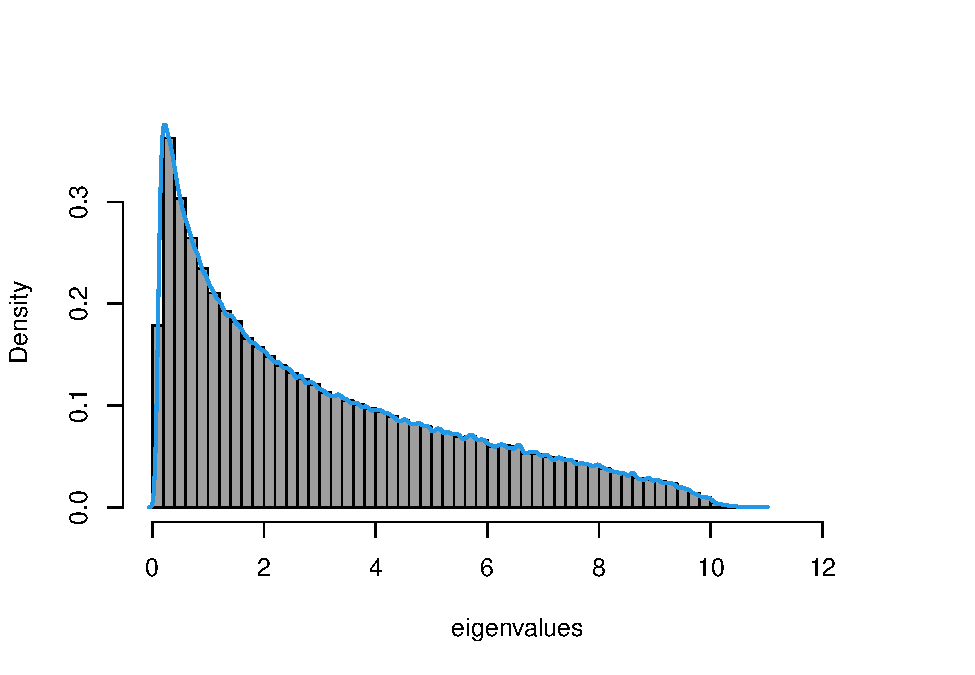
\includegraphics{A5_files/figure-latex/unnamed-chunk-43-1.pdf}

\begin{Shaded}
\begin{Highlighting}[]
\CommentTok{\# Define a function representing the kernel density estimate}
\NormalTok{kde\_func }\OtherTok{\textless{}{-}} \FunctionTok{approxfun}\NormalTok{(d}\SpecialCharTok{$}\NormalTok{x, d}\SpecialCharTok{$}\NormalTok{y, }\AttributeTok{method=}\StringTok{"linear"}\NormalTok{, }\AttributeTok{rule=}\DecValTok{2}\NormalTok{)}

\CommentTok{\# Define the integrand for the second moment}
\NormalTok{integrand }\OtherTok{\textless{}{-}} \ControlFlowTok{function}\NormalTok{(x) \{}
\NormalTok{  x}\SpecialCharTok{\^{}}\DecValTok{2} \SpecialCharTok{*} \FunctionTok{kde\_func}\NormalTok{(x)}
\NormalTok{\}}

\CommentTok{\# Integrate over the range of the data}
\NormalTok{second\_moment\_result }\OtherTok{\textless{}{-}} \FunctionTok{quadgk}\NormalTok{(integrand, }
                   \AttributeTok{a =} \FunctionTok{min}\NormalTok{(eigenvalues), }\CommentTok{\# We consider the positive (semi)definite matrix YY\^{}T/m}
                   \AttributeTok{b =} \FunctionTok{max}\NormalTok{(eigenvalues))}

\CommentTok{\# Print the result}
\FunctionTok{print}\NormalTok{(second\_moment\_result)}
\end{Highlighting}
\end{Shaded}

\begin{verbatim}
## [1] 15.51741
\end{verbatim}

\begin{Shaded}
\begin{Highlighting}[]
\NormalTok{n\_sims }\OtherTok{=} \DecValTok{1000}
\NormalTok{beta\_2\_hat }\OtherTok{=} \FunctionTok{future\_replicate}\NormalTok{(n\_sims, \{}
\NormalTok{  X }\OtherTok{=} \FunctionTok{GMM}\NormalTok{(n, p, }\FunctionTok{diag}\NormalTok{(p), rxi)}
\NormalTok{  Sn }\OtherTok{=} \FunctionTok{cov}\NormalTok{(X)}
\NormalTok{  L}\OtherTok{=}\FunctionTok{eigen}\NormalTok{(Sn, }\AttributeTok{only.values =} \ConstantTok{TRUE}\NormalTok{)}\SpecialCharTok{$}\NormalTok{values}
\NormalTok{  LSS }\OtherTok{=} \FunctionTok{sum}\NormalTok{(L}\SpecialCharTok{\^{}}\DecValTok{2}\NormalTok{)}\SpecialCharTok{/}\NormalTok{p}
\NormalTok{\})}
\end{Highlighting}
\end{Shaded}

\begin{Shaded}
\begin{Highlighting}[]
\NormalTok{LLS\_normalized }\OtherTok{=}\NormalTok{ (}\FunctionTok{sqrt}\NormalTok{(p)}\SpecialCharTok{*}\NormalTok{(beta\_2\_hat }\SpecialCharTok{{-}}\NormalTok{second\_moment\_result) }\SpecialCharTok{{-}}\NormalTok{ mu)}\SpecialCharTok{/}\NormalTok{Sigma}
\FunctionTok{qqnorm}\NormalTok{(LLS\_normalized, }\AttributeTok{main =} \StringTok{"QQ{-}Plot of LLS against N(0,1)"}\NormalTok{, }\AttributeTok{ylab =} \StringTok{"Quantiles of LLS"}\NormalTok{, }\AttributeTok{xlab =} \StringTok{"Quantiles of N(0,1)"}\NormalTok{)}
\FunctionTok{qqline}\NormalTok{(LLS\_normalized, }\AttributeTok{col =} \StringTok{"red"}\NormalTok{, }\AttributeTok{lwd =} \DecValTok{2}\NormalTok{)}
\end{Highlighting}
\end{Shaded}

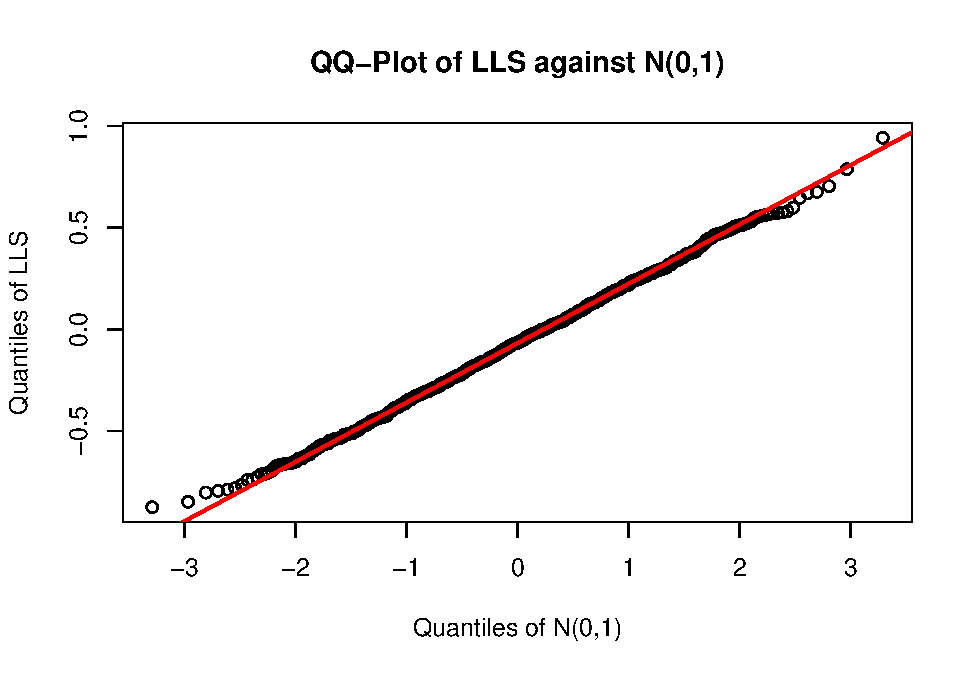
\includegraphics{A5_files/figure-latex/unnamed-chunk-45-1.pdf}

Now we can simulation the GMM in case where \(p =600, n = 900\).

\begin{Shaded}
\begin{Highlighting}[]
\NormalTok{p }\OtherTok{=} \DecValTok{600}
\NormalTok{n }\OtherTok{=} \DecValTok{900}
\NormalTok{mu }\OtherTok{=}\NormalTok{ mu1}\SpecialCharTok{/}\FunctionTok{sqrt}\NormalTok{(p) }\SpecialCharTok{+}\NormalTok{ mu2}
\NormalTok{Sigma }\OtherTok{=}\NormalTok{ Sigma1}\SpecialCharTok{/}\NormalTok{p }\SpecialCharTok{+}\NormalTok{ Sigma2}
\NormalTok{mu}
\end{Highlighting}
\end{Shaded}

\begin{verbatim}
## [1] 0.2561235
\end{verbatim}

\begin{Shaded}
\begin{Highlighting}[]
\NormalTok{Sigma}
\end{Highlighting}
\end{Shaded}

\begin{verbatim}
## [1] 10.18838
\end{verbatim}

\begin{Shaded}
\begin{Highlighting}[]
\NormalTok{n\_sims }\OtherTok{=} \DecValTok{1000}
\NormalTok{eigenvalues }\OtherTok{=} \FunctionTok{future\_replicate}\NormalTok{(n\_sims, \{}
\NormalTok{  X }\OtherTok{=} \FunctionTok{GMM}\NormalTok{(n, p, }\FunctionTok{diag}\NormalTok{(p), rxi)}
\NormalTok{  Sn }\OtherTok{=} \FunctionTok{cov}\NormalTok{(X)}
\NormalTok{  L}\OtherTok{=}\FunctionTok{eigen}\NormalTok{(Sn, }\AttributeTok{only.values =} \ConstantTok{TRUE}\NormalTok{)}\SpecialCharTok{$}\NormalTok{values}
\NormalTok{\})}
\NormalTok{d }\OtherTok{=} \FunctionTok{density}\NormalTok{(eigenvalues, }\AttributeTok{bw=}\StringTok{"SJ"}\NormalTok{, }\AttributeTok{kernel=}\StringTok{"gaussian"}\NormalTok{)}
\FunctionTok{hist}\NormalTok{(eigenvalues, }\AttributeTok{breaks=}\DecValTok{50}\NormalTok{, }\AttributeTok{xlim=}\FunctionTok{c}\NormalTok{(}\DecValTok{0}\NormalTok{,}\FloatTok{1.2}\SpecialCharTok{*}\FunctionTok{max}\NormalTok{(eigenvalues)), }\AttributeTok{freq=}\ConstantTok{FALSE}\NormalTok{, }\AttributeTok{col=}\DecValTok{8}\NormalTok{, }\AttributeTok{main=}\StringTok{\textquotesingle{}\textquotesingle{}}\NormalTok{)}
\FunctionTok{lines}\NormalTok{(d, }\AttributeTok{col=}\DecValTok{4}\NormalTok{, }\AttributeTok{lwd=}\DecValTok{2}\NormalTok{)}
\end{Highlighting}
\end{Shaded}

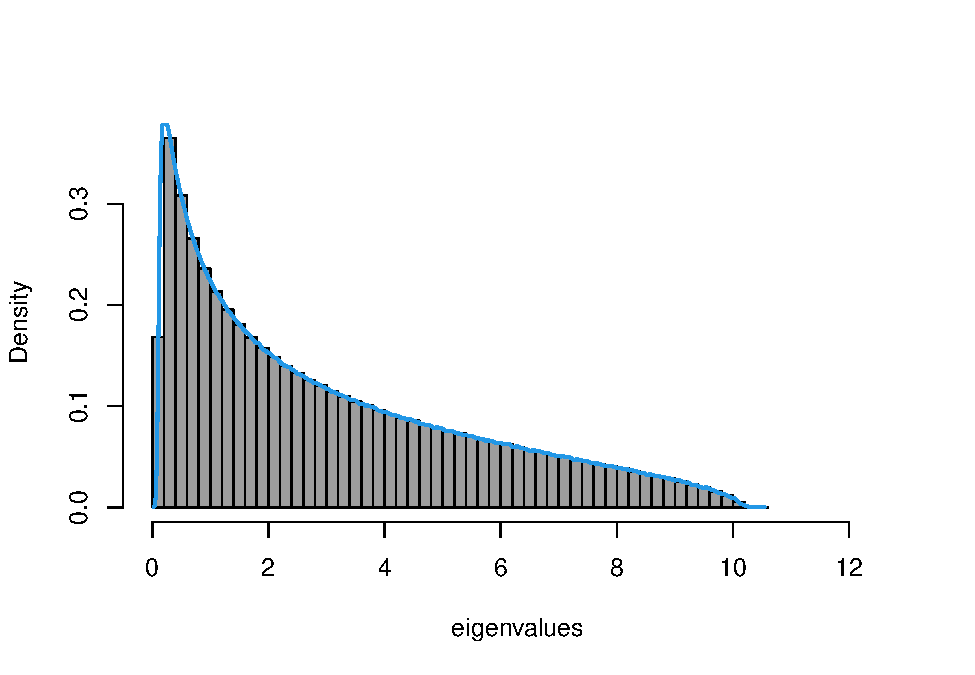
\includegraphics{A5_files/figure-latex/unnamed-chunk-47-1.pdf}

\begin{Shaded}
\begin{Highlighting}[]
\CommentTok{\# Define a function representing the kernel density estimate}
\NormalTok{kde\_func }\OtherTok{\textless{}{-}} \FunctionTok{approxfun}\NormalTok{(d}\SpecialCharTok{$}\NormalTok{x, d}\SpecialCharTok{$}\NormalTok{y, }\AttributeTok{method=}\StringTok{"linear"}\NormalTok{, }\AttributeTok{rule=}\DecValTok{2}\NormalTok{)}

\CommentTok{\# Define the integrand for the second moment}
\NormalTok{integrand }\OtherTok{\textless{}{-}} \ControlFlowTok{function}\NormalTok{(x) \{}
\NormalTok{  x}\SpecialCharTok{\^{}}\DecValTok{2} \SpecialCharTok{*} \FunctionTok{kde\_func}\NormalTok{(x)}
\NormalTok{\}}

\CommentTok{\# Integrate over the range of the data}
\NormalTok{second\_moment\_result }\OtherTok{\textless{}{-}} \FunctionTok{quadgk}\NormalTok{(integrand, }
                   \AttributeTok{a =} \FunctionTok{min}\NormalTok{(eigenvalues), }\CommentTok{\# We consider the positive (semi)definite matrix YY\^{}T/m}
                   \AttributeTok{b =} \FunctionTok{max}\NormalTok{(eigenvalues))}

\CommentTok{\# Print the result}
\FunctionTok{print}\NormalTok{(second\_moment\_result)}
\end{Highlighting}
\end{Shaded}

\begin{verbatim}
## [1] 15.54385
\end{verbatim}

\begin{Shaded}
\begin{Highlighting}[]
\NormalTok{n\_sims }\OtherTok{=} \DecValTok{1000}
\NormalTok{beta\_2\_hat }\OtherTok{=} \FunctionTok{future\_replicate}\NormalTok{(n\_sims, \{}
\NormalTok{  X }\OtherTok{=} \FunctionTok{GMM}\NormalTok{(n, p, }\FunctionTok{diag}\NormalTok{(p), rxi)}
\NormalTok{  Sn }\OtherTok{=} \FunctionTok{cov}\NormalTok{(X)}
\NormalTok{  L}\OtherTok{=}\FunctionTok{eigen}\NormalTok{(Sn, }\AttributeTok{only.values =} \ConstantTok{TRUE}\NormalTok{)}\SpecialCharTok{$}\NormalTok{values}
\NormalTok{  LSS }\OtherTok{=} \FunctionTok{sum}\NormalTok{(L}\SpecialCharTok{\^{}}\DecValTok{2}\NormalTok{)}\SpecialCharTok{/}\NormalTok{p}
\NormalTok{\})}
\NormalTok{LLS\_normalized }\OtherTok{=}\NormalTok{ (}\FunctionTok{sqrt}\NormalTok{(p)}\SpecialCharTok{*}\NormalTok{(beta\_2\_hat }\SpecialCharTok{{-}}\NormalTok{second\_moment\_result) }\SpecialCharTok{{-}}\NormalTok{ mu)}\SpecialCharTok{/}\NormalTok{Sigma}
\FunctionTok{qqnorm}\NormalTok{(LLS\_normalized, }\AttributeTok{main =} \StringTok{"QQ{-}Plot of LLS against N(0,1)"}\NormalTok{, }\AttributeTok{ylab =} \StringTok{"Quantiles of LLS"}\NormalTok{, }\AttributeTok{xlab =} \StringTok{"Quantiles of N(0,1)"}\NormalTok{)}
\FunctionTok{qqline}\NormalTok{(LLS\_normalized, }\AttributeTok{col =} \StringTok{"red"}\NormalTok{, }\AttributeTok{lwd =} \DecValTok{2}\NormalTok{)}
\end{Highlighting}
\end{Shaded}

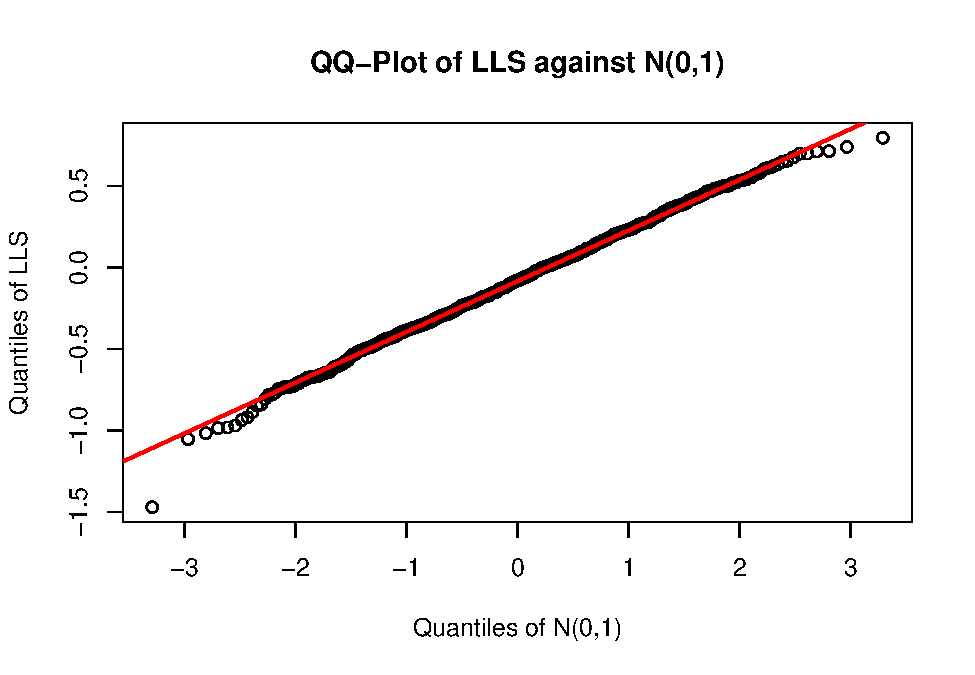
\includegraphics{A5_files/figure-latex/unnamed-chunk-48-1.pdf}

\begin{Shaded}
\begin{Highlighting}[]
\FunctionTok{rm}\NormalTok{(}\AttributeTok{list=}\FunctionTok{ls}\NormalTok{())}
\end{Highlighting}
\end{Shaded}

\begin{enumerate}
\def\labelenumi{(\alph{enumi})}
\setcounter{enumi}{2}
\tightlist
\item
  In addition to Question 2 (d), also reproduce the simulation
  experiment shown in Table 7 of {[}F{]} for the case
  \(\frac{p}{n} = 0.5\) and only for LR-SN and JHN-SN for
  \(p = 100, 200, 500\). Do this in the case of 1,000 replications.
\end{enumerate}

\paragraph{\texorpdfstring{\textbf{Answer to question 3
(c)}:}{Answer to question 3 (c):}}\label{answer-to-question-3-c}

\begin{Shaded}
\begin{Highlighting}[]
\FunctionTok{library}\NormalTok{(pracma)}
\NormalTok{rellipse\_normalised }\OtherTok{\textless{}{-}} \ControlFlowTok{function}\NormalTok{(n, p, }\AttributeTok{Sigma =} \FunctionTok{diag}\NormalTok{(p))\{}
  \CommentTok{\# Calculate Z\_ij from t with dof 4}
\NormalTok{  Z }\OtherTok{\textless{}{-}} \FunctionTok{matrix}\NormalTok{(}\FunctionTok{rt}\NormalTok{(n }\SpecialCharTok{*}\NormalTok{ p, }\AttributeTok{df =} \DecValTok{4}\NormalTok{), }\AttributeTok{ncol =}\NormalTok{ p)}
  
  \CommentTok{\# Calculate omega\_i}
\NormalTok{  omega }\OtherTok{\textless{}{-}} \FunctionTok{numeric}\NormalTok{(n)}
\NormalTok{  omega[}\DecValTok{1}\NormalTok{] }\OtherTok{\textless{}{-}} \FloatTok{0.01}  \CommentTok{\# assuming initial value of omega is 1, can be changed}
  \ControlFlowTok{for}\NormalTok{ (i }\ControlFlowTok{in} \DecValTok{2}\SpecialCharTok{:}\NormalTok{n) \{}
\NormalTok{    omega\_squared }\OtherTok{\textless{}{-}} \FloatTok{0.01} \SpecialCharTok{+} \FloatTok{0.85} \SpecialCharTok{*}\NormalTok{ omega[i }\SpecialCharTok{{-}} \DecValTok{1}\NormalTok{]}\SpecialCharTok{\^{}}\DecValTok{2} \SpecialCharTok{+} \FloatTok{0.1} \SpecialCharTok{*} \FunctionTok{sum}\NormalTok{(Z[i }\SpecialCharTok{{-}} \DecValTok{1}\NormalTok{, ]}\SpecialCharTok{\^{}}\DecValTok{2}\NormalTok{) }\SpecialCharTok{/} \FunctionTok{sum}\NormalTok{(}\FunctionTok{diag}\NormalTok{(Sigma))}
\NormalTok{    omega[i] }\OtherTok{\textless{}{-}}  \FunctionTok{sqrt}\NormalTok{(omega\_squared)}
\NormalTok{  \}}

  \CommentTok{\# Compute x}
\NormalTok{  A }\OtherTok{\textless{}{-}} \FunctionTok{sqrtm}\NormalTok{(Sigma)}
\NormalTok{  Y }\OtherTok{\textless{}{-}}\NormalTok{ omega}\SpecialCharTok{*}\FunctionTok{t}\NormalTok{(A}\SpecialCharTok{$}\NormalTok{B}\SpecialCharTok{\%*\%}\FunctionTok{t}\NormalTok{(Z)) }\CommentTok{\# (n, p)}
  
  \CommentTok{\# Compute the Euclidean norm for each row}
\NormalTok{  row\_norms }\OtherTok{\textless{}{-}} \FunctionTok{apply}\NormalTok{(Y, }\DecValTok{1}\NormalTok{, }\ControlFlowTok{function}\NormalTok{(Y\_i) }\FunctionTok{sqrt}\NormalTok{(}\FunctionTok{sum}\NormalTok{(Y\_i}\SpecialCharTok{\^{}}\DecValTok{2}\NormalTok{)))}

  \CommentTok{\# Normalize each row}
\NormalTok{  normalized\_Y }\OtherTok{\textless{}{-}}\NormalTok{ Y}\SpecialCharTok{/}\NormalTok{row\_norms}
  
  \FunctionTok{return}\NormalTok{(normalized\_Y)}
\NormalTok{\}}
\NormalTok{pcor }\OtherTok{=} \ControlFlowTok{function}\NormalTok{(rho, p) \{}
\NormalTok{  Tn }\OtherTok{=} \FunctionTok{matrix}\NormalTok{(}\DecValTok{0}\NormalTok{, p, p)}
  \ControlFlowTok{for}\NormalTok{ (i }\ControlFlowTok{in} \DecValTok{1}\SpecialCharTok{:}\NormalTok{p) \{}
    \ControlFlowTok{for}\NormalTok{ (j }\ControlFlowTok{in} \DecValTok{1}\SpecialCharTok{:}\NormalTok{p) \{}
\NormalTok{      Tn[i,j] }\OtherTok{=}\NormalTok{ rho}\SpecialCharTok{\^{}}\FunctionTok{abs}\NormalTok{(i}\SpecialCharTok{{-}}\NormalTok{j)}
\NormalTok{    \}}
\NormalTok{  \}}
  \FunctionTok{return}\NormalTok{(Tn)}
\NormalTok{\}}
\end{Highlighting}
\end{Shaded}

\begin{Shaded}
\begin{Highlighting}[]
\NormalTok{y }\OtherTok{=} \DecValTok{1}\SpecialCharTok{/}\DecValTok{2}
\NormalTok{p\_list }\OtherTok{=} \FunctionTok{c}\NormalTok{(}\DecValTok{100}\NormalTok{, }\DecValTok{200}\NormalTok{, }\DecValTok{500}\NormalTok{)}
\NormalTok{alpha }\OtherTok{\textless{}{-}} \FloatTok{0.05}
\end{Highlighting}
\end{Shaded}

\begin{Shaded}
\begin{Highlighting}[]
\FunctionTok{plan}\NormalTok{(multisession, }\AttributeTok{workers =} \DecValTok{8}\NormalTok{)}
\NormalTok{n\_sims }\OtherTok{=} \DecValTok{1000}
\NormalTok{LRSN\_simulation }\OtherTok{\textless{}{-}} \ControlFlowTok{function}\NormalTok{(n\_sims, p, y)\{}
\NormalTok{  t\_LRSN }\OtherTok{=} \FunctionTok{future\_replicate}\NormalTok{(n\_sims, \{}
\NormalTok{    n }\OtherTok{=}\NormalTok{ p}\SpecialCharTok{/}\NormalTok{y}
\NormalTok{    Sigma }\OtherTok{=} \FunctionTok{pcor}\NormalTok{(}\FloatTok{0.1}\NormalTok{, p)}
\NormalTok{    X }\OtherTok{=} \FunctionTok{rellipse\_normalised}\NormalTok{(n, p, Sigma)}
\NormalTok{    Sn }\OtherTok{=} \FunctionTok{sum}\NormalTok{(}\FunctionTok{diag}\NormalTok{(Sigma))}\SpecialCharTok{*}\FunctionTok{t}\NormalTok{(X)}\SpecialCharTok{\%*\%}\NormalTok{X}\SpecialCharTok{/}\NormalTok{n}
\NormalTok{    L }\OtherTok{=} \FunctionTok{eigen}\NormalTok{(Sn, }\AttributeTok{only.values =} \ConstantTok{TRUE}\NormalTok{)}\SpecialCharTok{$}\NormalTok{values}
\NormalTok{    L\_ }\OtherTok{=} \FunctionTok{sum}\NormalTok{(}\FunctionTok{log}\NormalTok{(L))}
\NormalTok{    mu\_LRSN }\OtherTok{=}\NormalTok{ p}\SpecialCharTok{*}\NormalTok{(((y }\SpecialCharTok{{-}} \DecValTok{1}\NormalTok{)}\SpecialCharTok{/}\NormalTok{y) }\SpecialCharTok{*}\FunctionTok{log}\NormalTok{(}\DecValTok{1} \SpecialCharTok{{-}}\NormalTok{ y) }\SpecialCharTok{{-}} \DecValTok{1}\NormalTok{) }\SpecialCharTok{+} \FunctionTok{log}\NormalTok{(}\DecValTok{1} \SpecialCharTok{{-}}\NormalTok{ y)}\SpecialCharTok{/}\DecValTok{2} \SpecialCharTok{+}\NormalTok{ y}
\NormalTok{    sd\_LRSN }\OtherTok{=} \FunctionTok{sqrt}\NormalTok{(}\SpecialCharTok{{-}}\DecValTok{2}\SpecialCharTok{*}\FunctionTok{log}\NormalTok{(}\DecValTok{1} \SpecialCharTok{{-}}\NormalTok{ y) }\SpecialCharTok{{-}} \DecValTok{2}\SpecialCharTok{*}\NormalTok{y)}
\NormalTok{    LRSN }\OtherTok{=}\NormalTok{ (L\_ }\SpecialCharTok{{-}}\NormalTok{ mu\_LRSN)}\SpecialCharTok{/}\NormalTok{sd\_LRSN}
\NormalTok{    \})}
\NormalTok{\}}

\ControlFlowTok{for}\NormalTok{(i }\ControlFlowTok{in} \DecValTok{1}\SpecialCharTok{:}\FunctionTok{length}\NormalTok{(p\_list))\{}
\NormalTok{  t\_LRSN }\OtherTok{\textless{}{-}} \FunctionTok{LRSN\_simulation}\NormalTok{(n\_sims, p\_list[i], y)}
\NormalTok{  critical\_left }\OtherTok{=} \FunctionTok{qnorm}\NormalTok{(alpha}\SpecialCharTok{/}\DecValTok{2}\NormalTok{)}
\NormalTok{  critical\_right }\OtherTok{=} \FunctionTok{qnorm}\NormalTok{(}\DecValTok{1} \SpecialCharTok{{-}}\NormalTok{ alpha}\SpecialCharTok{/}\DecValTok{2}\NormalTok{)}
\NormalTok{  mean.beta }\OtherTok{=} \FunctionTok{mean}\NormalTok{(t\_LRSN }\SpecialCharTok{\textgreater{}=}\NormalTok{ critical\_left }\SpecialCharTok{\&}\NormalTok{ t\_LRSN }\SpecialCharTok{\textless{}=}\NormalTok{ critical\_right)}
  \FunctionTok{cat}\NormalTok{(}\StringTok{"The test power is"}\NormalTok{, (}\DecValTok{1} \SpecialCharTok{{-}}\NormalTok{ mean.beta), }\StringTok{"when the dimension is"}\NormalTok{, p\_list[i],}\StringTok{"}\SpecialCharTok{\textbackslash{}n}\StringTok{"}\NormalTok{)}
\NormalTok{\}}
\end{Highlighting}
\end{Shaded}

\begin{verbatim}
## The test power is 0.347 when the dimension is 100 
## The test power is 0.859 when the dimension is 200 
## The test power is 1 when the dimension is 500
\end{verbatim}

\begin{Shaded}
\begin{Highlighting}[]
\NormalTok{n\_sims }\OtherTok{=} \DecValTok{1000}
\NormalTok{JHNSN\_simulation }\OtherTok{\textless{}{-}} \ControlFlowTok{function}\NormalTok{(n\_sims, p, y)\{}
\NormalTok{  t\_JHNSN }\OtherTok{=} \FunctionTok{future\_replicate}\NormalTok{(n\_sims, \{}
\NormalTok{    n }\OtherTok{=}\NormalTok{ p}\SpecialCharTok{/}\NormalTok{y}
\NormalTok{    Sigma }\OtherTok{=} \FunctionTok{pcor}\NormalTok{(}\FloatTok{0.1}\NormalTok{, p)}
\NormalTok{    X }\OtherTok{=} \FunctionTok{rellipse\_normalised}\NormalTok{(n, p, Sigma)}
\NormalTok{    Sn }\OtherTok{=} \FunctionTok{sum}\NormalTok{(}\FunctionTok{diag}\NormalTok{(Sigma))}\SpecialCharTok{*}\FunctionTok{t}\NormalTok{(X)}\SpecialCharTok{\%*\%}\NormalTok{X}\SpecialCharTok{/}\NormalTok{n}
\NormalTok{    L }\OtherTok{=} \FunctionTok{eigen}\NormalTok{(Sn, }\AttributeTok{only.values =} \ConstantTok{TRUE}\NormalTok{)}\SpecialCharTok{$}\NormalTok{values}
\NormalTok{    L\_ }\OtherTok{=} \FunctionTok{sum}\NormalTok{(L}\SpecialCharTok{\^{}}\DecValTok{2}\NormalTok{)}
\NormalTok{    Tn }\OtherTok{=}\NormalTok{ L\_}\SpecialCharTok{/}\NormalTok{y }\SpecialCharTok{{-}}\NormalTok{ n }\SpecialCharTok{{-}}\NormalTok{ p}
\NormalTok{    JHNSN }\OtherTok{=}\NormalTok{ (Tn}\SpecialCharTok{+}\DecValTok{1}\NormalTok{)}\SpecialCharTok{/}\DecValTok{2}
\NormalTok{    \})}
\NormalTok{\}}

\ControlFlowTok{for}\NormalTok{(i }\ControlFlowTok{in} \DecValTok{1}\SpecialCharTok{:}\FunctionTok{length}\NormalTok{(p\_list))\{}
\NormalTok{  t\_JHNSN }\OtherTok{\textless{}{-}} \FunctionTok{JHNSN\_simulation}\NormalTok{(n\_sims, p\_list[i], y)}
\NormalTok{  critical\_left }\OtherTok{=} \FunctionTok{qnorm}\NormalTok{(alpha}\SpecialCharTok{/}\DecValTok{2}\NormalTok{)}
\NormalTok{  critical\_right }\OtherTok{=} \FunctionTok{qnorm}\NormalTok{(}\DecValTok{1} \SpecialCharTok{{-}}\NormalTok{ alpha}\SpecialCharTok{/}\DecValTok{2}\NormalTok{)}
\NormalTok{  mean.beta }\OtherTok{=} \FunctionTok{mean}\NormalTok{(t\_JHNSN }\SpecialCharTok{\textgreater{}=}\NormalTok{ critical\_left }\SpecialCharTok{\&}\NormalTok{ t\_JHNSN }\SpecialCharTok{\textless{}=}\NormalTok{ critical\_right)}
  \FunctionTok{cat}\NormalTok{(}\StringTok{"The test power is"}\NormalTok{, (}\DecValTok{1} \SpecialCharTok{{-}}\NormalTok{ mean.beta), }\StringTok{"when the dimension is"}\NormalTok{, p\_list[i],}\StringTok{"}\SpecialCharTok{\textbackslash{}n}\StringTok{"}\NormalTok{)}
\NormalTok{\}}
\end{Highlighting}
\end{Shaded}

\begin{verbatim}
## The test power is 0.474 when the dimension is 100 
## The test power is 0.974 when the dimension is 200 
## The test power is 1 when the dimension is 500
\end{verbatim}

\begin{Shaded}
\begin{Highlighting}[]
\FunctionTok{rm}\NormalTok{(}\AttributeTok{list=}\FunctionTok{ls}\NormalTok{())}
\end{Highlighting}
\end{Shaded}


\end{document}
